\documentclass[12pt]{report}
\ifdefined\pdfminorversion
  \pdfminorversion=7
\fi

\usepackage[utf8]{inputenc}
\usepackage[T1]{fontenc}
\usepackage{lmodern}
\usepackage{graphicx}
\usepackage[table]{xcolor}
\usepackage{tikz}
\usepackage{fancyhdr}
\usepackage{hyperref}

% Keep links clickable without visible boxes and reduce line-breaking pressure
% after disabling automatic word hyphenation.
\hypersetup{
  hidelinks,
  colorlinks=false,
  pdfborder={0 0 0}
}
\emergencystretch=3em
\hyphenpenalty=10000
\exhyphenpenalty=10000
\brokenpenalty=10000

\makeatletter
% Prevent stretched spacing in headings by using ragged-right section styles.
\renewcommand\section{\@startsection{section}{1}{\z@}%
  {-3.5ex \@plus -1ex \@minus -.2ex}%
  {2.3ex \@plus.2ex}%
  {\normalfont\Large\bfseries\raggedright}}
\renewcommand\subsection{\@startsection{subsection}{2}{\z@}%
  {-3.25ex\@plus -1ex \@minus -.2ex}%
  {1.5ex \@plus .2ex}%
  {\normalfont\large\bfseries\raggedright}}
\renewcommand\subsubsection{\@startsection{subsubsection}{3}{\z@}%
  {-3.25ex\@plus -1ex \@minus -.2ex}%
  {1.5ex \@plus .2ex}%
  {\normalfont\normalsize\bfseries\raggedright}}

% Keep multi-line captions naturally wrapped instead of fully justified.
\long\def\@makecaption#1#2{%
  \vskip\abovecaptionskip
  \sbox\@tempboxa{\small\textbf{#1.} #2}%
  \ifdim \wd\@tempboxa >\hsize
    {\small\raggedright\textbf{#1.} #2\par}%
  \else
    \global \@minipagefalse
    \hb@xt@\hsize{\hfil\box\@tempboxa\hfil}%
  \fi
  \vskip\belowcaptionskip}
\makeatother

\usetikzlibrary{arrows.meta,positioning,shapes.geometric}

\setlength{\headheight}{18pt}

\fancypagestyle{thesismain}{
  \fancyhf{}
  \renewcommand{\chaptermark}[1]{\markboth{Chapter \thechapter. ##1}{}}
  \renewcommand{\sectionmark}[1]{}
  \fancyhead[L]{\small\nouppercase{\leftmark}}
  \fancyhead[R]{\small\thepage}
  \renewcommand{\headrulewidth}{0.4pt}
}

\fancypagestyle{plain}{
  \fancyhf{}
  \fancyfoot[C]{\thepage}
  \renewcommand{\headrulewidth}{0pt}
}

\newlength{\chaptercontentsrefwidth}
\setlength{\chaptercontentsrefwidth}{0.2\textwidth}

\newcommand{\chaptercontentsitem}[1]{%
  \par\noindent
  \parbox[t]{\dimexpr\linewidth-\chaptercontentsrefwidth\relax}{%
    \raggedright
    \strut\nameref{#1}\nobreak\leaders\hbox to 0.45em{\hss.\hss}\hfill\strut
  }%
  \nobreak\hfill
  \parbox[t]{\chaptercontentsrefwidth}{%
    \raggedleft\strut\ref*{#1}, p.~\pageref*{#1}\strut
  }%
  \par\vspace{0.2\baselineskip}
}

\newcommand{\chapteropeningcontents}[1]{%
  \vspace{1.5\baselineskip}%
  \begin{center}
    \begin{minipage}{0.84\textwidth}
      {\large\bfseries Contents\par}
      \vspace{0.8\baselineskip}
      \begingroup
        \setlength{\parindent}{0pt}%
        \setlength{\parskip}{0.15\baselineskip}%
        #1
      \endgroup
    \end{minipage}
  \end{center}
  \clearpage
}

\newcommand{\chapterwithopening}[3]{%
  \chapter{#1}%
  \label{#2}%
  \chapteropeningcontents{#3}%
}

\begin{document}

\pagenumbering{roman}

\chapter*{Abstract}
\addcontentsline{toc}{chapter}{Abstract}

EduVerse is presented in this thesis as an integrated educational platform
designed to reduce the fragmentation that commonly arises when class
communication, learning materials, live meetings, whiteboard collaboration,
programming practice, assessment, and academic follow-up are distributed across
separate tools. The platform follows a multi-organization, role-based model in
which Organization Administrators, Teachers, and Students operate within a
governed workspace that can adapt to different institutional needs. Within that
workspace, EduVerse supports classes, materials, chat, assignments, exams,
results, notifications, live sessions, whiteboard collaboration, an AI Agent,
an integrated browser-based IDE, configurable feature availability, extension
support, and public or open-learning access where enabled.

The main implementation is a web platform built with Next.js, React, and
TypeScript. It uses Supabase for authentication and relational data, AWS S3 for
file storage, LiveKit for live-session participation, and OpenRouter for
AI-supported learning services. EduVerse also includes a mobile companion
application implemented with Expo, React Native, and TypeScript. The current
mobile client provides authenticated access, class summaries, notifications,
materials, class chat, organization switching, and basic live-session
participation. However, it remains under active development and is not a full
replacement for the web platform, where broader administrative and advanced
learning workflows are still concentrated.

The thesis documents the problem context, system analysis, design,
implementation, and evaluation of EduVerse using the available implementation
evidence, project documentation, and targeted validation. The evaluation shows
credible support for role-based academic workflows, shared API reuse, modular
feature enablement, and integrated educational services, while also identifying
realistic limitations in end-to-end testing breadth and in the current scope of
the mobile companion. Overall, EduVerse contributes a coherent and extensible
approach to building a governed digital learning environment around one
connected academic platform rather than a collection of disconnected tools.

\chapter*{Acknowledgements}
\addcontentsline{toc}{chapter}{Acknowledgements}

All praise and gratitude are due to Allah, whose guidance, mercy, and blessings
made it possible for us to complete this work. We are deeply thankful for the
strength, patience, and perseverance that carried us through the challenges of
this project and throughout our studies.

We would like to express our sincere gratitude to our parents and families for
their constant encouragement, sacrifice, and unwavering support. Their trust,
patience, and belief in us provided the foundation that enabled us to continue
and complete this journey.

We are especially grateful to our supervisor, Dr. Khari Amir Armih, for his
guidance, valuable advice, and continued support throughout the development of
this graduation project. His direction helped us strengthen both the quality of
the project itself and the discipline with which we approached our work.

We also extend our appreciation to the EduVerse project team for the
collaboration, effort, and shared commitment invested in this work. Developing
the project required patience, cooperation, and sustained problem solving, and
we are grateful for the spirit of teamwork that made its completion possible.


\tableofcontents
\listoffigures
\listoftables

\clearpage
\pagenumbering{arabic}
\pagestyle{thesismain}

\chapterwithopening{Strategic Vision and Project Scope}{chap:strategic_vision}{
  \chaptercontentsitem{sec:project_vision}
  \chaptercontentsitem{sec:problem_statement}
  \chaptercontentsitem{sec:project_motivations}
  \chaptercontentsitem{sec:strategic_objectives}
  \chaptercontentsitem{sec:team_goals}
  \chaptercontentsitem{sec:project_scope}
}

\section{Project Vision}\label{sec:project_vision}

Digital transformation has become a defining condition of contemporary
education. Institutions increasingly depend on online systems not only to store
materials, but also to coordinate communication, teaching, assessment,
feedback, collaboration, and daily academic follow-up across time and location.
As that dependence grows, the quality of the learning environment depends less
on the presence of isolated tools and more on whether those tools form a
coherent academic system.

Within this broader context, educational workflows often remain fragmented.
Class communication may occur in one platform, materials in another, live
teaching in another, and practical technical work elsewhere. EduVerse is
proposed as a response to that condition: an integrated educational platform
that brings related academic workflows into one governed digital environment
instead of leaving them scattered across loosely connected services.

This strategic direction is intentionally broader than any single institutional
type. EduVerse is conceived as a governed academic environment that can serve
universities, schools, online academies, bootcamps, tutoring centers,
exam-preparation spaces, corporate training contexts, and open-learning
communities without assuming that all of them need the same configuration.

Its vision is shaped by two practical goals. The first is to provide a
coherent digital environment in which related academic work can remain
connected. The second is to preserve adaptability, so that organizations and
classes can enable, disable, extend, or restrict features according to their
own policies and teaching needs. EduVerse is therefore framed not as a fixed
bundle of tools, but as a configurable academic workspace designed for
continuity, governance, and long-term growth.

\section{Problem Statement}\label{sec:problem_statement}

Many educational workflows are currently distributed across separate systems.
One platform may be used for class communication and sharing materials, another
for live meetings and presentations, another for collaborative whiteboard
interaction, and another for programming practice. Familiar examples include
Google Classroom for announcements and materials, Google Meet for live calls,
Excalidraw-like tools for shared whiteboard work, and LeetCode-like
environments for coding exercises. While each tool can be useful on its own,
their separation introduces repeated context switching, inconsistent workflow
boundaries, weaker continuity between related academic tasks, and scattered
responsibility for governance and follow-up.

This fragmentation becomes more serious in multi-organization educational
settings. A platform must not only expose features; it must also manage roles,
permissions, memberships, public access rules, class visibility, and the
relationship between administrative governance and daily learning activity.
When these concerns are spread across unrelated services, both usability and
accountability become harder to maintain.

The problem also has a client-design dimension. Rich administrative workflows,
content management, assessment authoring, and complex class control are better
suited to a full web environment. At the same time, many high-frequency actions
such as checking updates, opening materials, reading chat, reviewing class
summaries, and joining live sessions should remain practical from mobile
devices. A realistic educational platform therefore needs both a strong primary
web application and a carefully scoped mobile companion rather than an
unstructured duplication of screens.

\section{Project Motivations}\label{sec:project_motivations}

EduVerse was motivated by the opportunity to build a digital learning
environment in which academic continuity and institutional control could be
designed together. Rather than treating governance, communication, assessment,
and learning support as loosely related concerns, the project aimed to realize
them within one environment that could remain useful across different
educational contexts.

The project was also academically and professionally valuable for the team. It
required the combination of requirements analysis, system modeling,
implementation, service integration, security-aware design, testing, and
technical reporting within one sustained engineering effort. In this sense,
EduVerse served not only as a software product, but also as a realistic
graduation project through which the team could practice disciplined
collaborative development.

\section{Strategic Objectives}\label{sec:strategic_objectives}

The strategic objectives of EduVerse translate the project vision into concrete
institutional and functional targets.

\begin{itemize}
  \item To provide a multi-organization educational platform that can support
    distinct institutions or organizational units within one governed system.
  \item To support role-based operation for Organization Administrators,
    Teachers, and Students, including users who belong to more than one
    organization or hold more than one role.
  \item To unify classes, materials, chat, assignments, exams, results,
    notifications, live sessions, whiteboard collaboration, AI support, and
    coding practice within one academic environment.
  \item To allow supported features to be enabled or disabled at organization
    level and, where appropriate, refined further at class level.
  \item To allow AI-supported features to be disabled for organizations or
    classes that do not wish to use them.
  \item To support public or open-learning access where enabled, so that
    organizations can share educational materials or membership paths more
    broadly without giving up institutional control.
  \item To support controlled extension and future integration so that new
    capabilities or external clients can reuse the same protected academic API
    model rather than rebuilding business rules from scratch.
  \item To provide a primary web platform for complete academic and
    administrative workflows while extending selected day-to-day actions
    through a mobile companion application.
\end{itemize}

\section{Educational and Professional Goals for the Team}\label{sec:team_goals}

For the project team, EduVerse represents a complete software engineering
exercise grounded in a realistic problem domain. The work required the team to
move from problem framing to requirements analysis, methodology selection,
system design, implementation, validation, and documentation in a coordinated
way.

The project also supported professional growth. It strengthened experience in
problem decomposition, collaborative planning, technical trade-off analysis,
review discipline, and responsibility for system quality. These outcomes are
important because the value of a graduation project lies not only in the final
software, but also in the maturity of the engineering process used to produce
it.

\section{Project Scope and Boundaries}\label{sec:project_scope}
\subsection{System Boundaries and User Roles}\label{subsec:system_boundaries_roles}

EduVerse operates through three principal human roles: Organization
Administrator, Teacher, and Student. The same person may hold more than one
role, and a user may belong to more than one organization. For that reason, the
system resolves access according to the selected organization, the active role,
class membership, and the current feature configuration rather than by assuming
that every user belongs to one fixed category.

This role structure defines an important project boundary. EduVerse is not a
general social platform in which all users share the same permissions. It is a
governed educational workspace in which visibility, management authority,
assessment control, and feature access are deliberately differentiated.

\subsection{Functional Scope}\label{subsec:functional_scope}

Within its implemented scope, EduVerse includes authentication, organization
access and membership, class management, materials, chat, assignments, exams,
results, notifications, live sessions, whiteboard collaboration, an AI Agent,
and an integrated coding workspace. It also includes organization-level and
class-level feature controls, extension support, and optional public or
open-learning access where those capabilities are enabled.

This scope is not restricted to higher education alone. The same model can be
adapted for primary schools and kindergartens through narrower feature
selection and closer organization-level control, just as it can support more
specialized contexts such as technical courses, tutoring programs, or open
learning initiatives.

The class model is intentionally flexible. A class can support a conventional
course, but it can also be used for a narrower academic purpose. For example, a
class may function as a digital library space dedicated mainly to sharing books
and learning materials. This flexibility shows that EduVerse is not restricted
to one teaching pattern; it is a configurable academic workspace that can be
adapted to different institutional uses.

\subsection{Web and Mobile Client Scope}\label{subsec:web_mobile_client_scope}

The EduVerse web application is the primary and most complete client. It
supports the broader administrative, instructional, and assessment workflows
that define the platform as a full educational system.

EduVerse Mobile already exists as a companion mobile application, developed to
extend selected platform features to mobile users. Its scope is intentionally
narrower than the web platform. The current mobile implementation supports
authenticated access, class summaries, notifications, materials, class chat,
organization switching, and basic live-session participation. It is therefore
best described as a companion under active development rather than as a
feature-complete replacement for the web platform. Administrative workflows and
several advanced learning features remain mainly web-side.

\subsection{Distinctive Features and Extensible Design}
\label{subsec:competitive_features_innovation}

EduVerse is distinctive because it combines integration with control. The
platform brings together communication, materials, live collaboration,
assessment, AI assistance, and coding practice, but it does so inside a
governed multi-organization model rather than through a loose collection of
independent tools.

Its extensible design is also central to the project. Supported features can be
enabled or disabled at organization level and, where supported, refined further
at class level. AI features can likewise be disabled when an organization or a
specific class considers them unsuitable. The same underlying API model also
creates reuse potential for future integrations or companion clients, because
core workflows are exposed through protected shared routes rather than being
hard-wired to one interface only.

Public access adds another important dimension. When enabled, public
organizations or public join paths can support broader sharing of educational
materials and more open learning participation, while still remaining under
organization-defined governance rules.

\chapterwithopening{Literature Review and Theoretical Framework}{chap:literature_review}{
  \chaptercontentsitem{sec:literature_review_introduction}
  \chaptercontentsitem{sec:evolution_of_digital_education_platforms}
  \chaptercontentsitem{sec:research_gap_integrated_ecosystem}
  \chaptercontentsitem{sec:artificial_intelligence_in_education}
  \chaptercontentsitem{sec:benchmarking_fragmented_vs_integrated}
  \chaptercontentsitem{sec:theoretical_technical_foundations_eduverse}
}

\section{Introduction}\label{sec:literature_review_introduction}

This literature review establishes the conceptual and technical foundations
relevant to EduVerse and situates the project within existing approaches to
digital education. Because the platform combines several forms of academic
activity, its theoretical basis extends across digital learning systems,
communication and synchronous teaching, artificial intelligence in education,
access control, mobile learning, and extensible platform design.

Together, these areas provide the basis for examining how educational
activities can remain coordinated while supporting different users,
institutional requirements, and modes of participation. The review also
identifies limitations in fragmented educational environments and the design
principles that motivate a more connected approach.

\section{Evolution of Digital Education Platforms}
\label{sec:evolution_of_digital_education_platforms}

\subsection{From Traditional Classroom Management to Digital Learning Systems}
\label{subsec:traditional_to_digital_learning_systems}

Educational management has gradually moved from paper-based and face-to-face
coordination toward persistent digital systems capable of organizing materials,
communication, submissions, and academic records at institutional scale.
Learning management systems emerged as part of this transition, providing
shared digital spaces through which teaching and learning could be organized
more consistently \cite{chugh2023edtech,bygstad2022digital}.

This transition also changed user expectations. Students and teachers
increasingly expect continuous access, asynchronous participation, traceable
communication, and structured academic follow-up rather than isolated
interactions \cite{chugh2023edtech}. Modern educational platforms are therefore
evaluated not only by their ability to store resources, but also by how
effectively they support ongoing academic activity.

\subsection{Limitations of Fragmented Learning Management Tools}
\label{subsec:limitations_of_fragmented_learning_management_tools}

Research on educational digitalization shows that institutions commonly rely
on combinations of specialized systems for learning management, communication,
synchronous teaching, collaboration, and practical work. Although individual
tools may perform their intended functions effectively, using multiple
disconnected environments can weaken continuity across academic activities and
increase coordination overhead \cite{bygstad2022digital,oecd2023outlook}.

Such fragmentation can require users to repeatedly move between separate
contexts while institutions manage permissions, visibility, communication, and
responsibility across different services. The resulting challenge is
maintaining consistent academic coordination when related activities are
distributed across separate tools
\cite{bygstad2022digital,oecd2023outlook}.

\section{Research Gap and Integrated Learning Ecosystems}
\label{sec:research_gap_integrated_ecosystem}

The gap relevant to EduVerse concerns coordinated operation across individual
educational tools. Existing systems can support communication,
learning resources, assessment, synchronous teaching, collaboration, and
practical work independently; however, institutions also require these
activities to operate within consistent boundaries of responsibility, access,
and academic context.

This creates a broader requirement for educational environments that combine
functional integration with institutional flexibility. Integration alone may be insufficient when different institutions or classes are expected to use the same capabilities in the same way. Conversely, flexibility becomes difficult to
manage when related workflows are distributed across unrelated systems.

EduVerse addresses this gap by adopting an integrated but configurable
educational model. The significance of this approach lies not in introducing
entirely new categories of educational tools, but in coordinating familiar
academic functions within a shared institutional context.

\section{Artificial Intelligence in Education}
\label{sec:artificial_intelligence_in_education}

Artificial intelligence has become increasingly relevant to education because
it can support explanation, summarization, drafting, and personalized academic
assistance when used within appropriate pedagogical boundaries
\cite{bond2024ai,labadze2023chatbots}. Its educational value, however, depends
not only on its ability to generate content, but also on how its use affects
teacher judgment, academic integrity, and the learner's engagement with source
material.

For EduVerse, this literature supports treating AI as a supplementary learning
capability rather than as a replacement for instructional authority or
established academic resources.

\subsection{Context-Aware Learning Assistance}
\label{subsec:context_aware_learning_assistance}

AI assistance is generally more useful when it is informed by the learner's
current academic context. Responses related to the active class, learning
material, or task can provide more relevant support than generic answers
detached from the educational setting
\cite{alsafari2024teaching,labadze2023chatbots}. Context awareness can therefore
improve both relevance and pedagogical alignment.

This principle supports the use of embedded AI assistance in EduVerse, where
learning support is intended to remain connected to the academic environment in
which it is requested.

\subsection{Material Summarization and Learning Support}
\label{subsec:material_summarization_and_learning_support}

Long or numerous educational resources can make it difficult for students to
quickly recover the structure and key ideas of a topic. AI-supported
summarization can assist by foregrounding important concepts and reducing the
effort required to re-enter complex material \cite{xie2025summarization}.

Such summaries should remain supportive rather than substitutive. In the
context of EduVerse, summarization is therefore treated as an aid for navigating
learning material rather than as a replacement for the original resource.

\subsection{Assessment and Feedback Support}
\label{subsec:assessment_and_feedback_support}

The literature indicates that AI can contribute to formative learning support,
drafting, and feedback-related activities when used within clear educational
boundaries \cite{labadze2023chatbots}. At the same time, unrestricted use can
weaken authentic assessment and blur the distinction between assistance and
task completion \cite{unesco2023genai,labadze2023chatbots}.

These concerns support a cautious role for AI within EduVerse. AI-assisted
learning should complement teacher-led assessment and study activities without
replacing instructional authority or undermining the integrity of assessed
work.

\section{Benchmarking: Fragmented Tools vs. Integrated EduVerse Approach}
\label{sec:benchmarking_fragmented_vs_integrated}

The purpose of this benchmarking comparison is not to rank individual products,
but to contrast two different organizational models for digital learning:
workflows distributed across specialized tools and workflows coordinated within
a shared educational environment.
Table~\ref{tab:fragmented_vs_integrated_eduverse} summarizes the main structural
differences relevant to EduVerse.

\begingroup
\footnotesize
\setlength{\tabcolsep}{4pt}
\renewcommand{\arraystretch}{1.15}
\begin{longtable}{|>{\raggedright\arraybackslash}p{0.17\textwidth}|>{\raggedright\arraybackslash}p{0.34\textwidth}|>{\raggedright\arraybackslash}p{0.34\textwidth}|}
\caption{Fragmented Educational Tools vs. Integrated EduVerse Approach}
\label{tab:fragmented_vs_integrated_eduverse} \\
\hline
\rowcolor{gray!15}
\textbf{Workflow Area} &
\textbf{Fragmented Reference Model} &
\textbf{Integrated EduVerse Approach} \\
\hline
\endfirsthead
\hline
\rowcolor{gray!15}
\textbf{Workflow Area} &
\textbf{Fragmented Reference Model} &
\textbf{Integrated EduVerse Approach} \\
\hline
\endhead
\hline
\multicolumn{3}{r}{\small\textit{Continued on the next page}} \\
\endfoot
\hline
\endlastfoot
Learning Content and Communication &
Learning resources, announcements, communication, and related class activity
may be distributed across different systems, requiring users to move repeatedly
between contexts. &
Learning content and class communication remain connected to the same
organizational and class context. \\
\hline
Synchronous Collaboration &
Live teaching, presentation interaction, and collaborative whiteboard activity
may depend on separate communication and collaboration tools. &
Synchronous learning and collaborative activity remain associated with the
surrounding class environment. \\
\hline
Assessment and Practical Learning &
Assignments, examinations, results, and practical activities such as programming
may be handled through separate academic or specialist systems. &
Assessment and supported practical learning activities can remain connected to
the wider academic workflow. \\
\hline
Governance and Configurability &
Roles, permissions, visibility, and available capabilities may need to be
managed separately across different services. &
Institutional governance and supported feature configuration are coordinated
within the same educational environment. \\
\hline
Integration and Extension &
Extending a distributed environment may require additional integration between
independent systems and duplicated coordination logic. &
A shared platform model provides a common foundation for supported extensions
and connected clients. \\
\hline
\end{longtable}
\endgroup

The comparison indicates that the main distinction lies in coordination across
related academic activities rather than in any single feature. EduVerse
therefore draws its value from the relationship between these capabilities and
the institutional context in which they operate.

\section{Theoretical and Technical Foundations of EduVerse}
\label{sec:theoretical_technical_foundations_eduverse}

The preceding literature identifies several principles relevant to the design
of an integrated educational environment. The following subsections summarize
the foundations most directly related to EduVerse, including web-based
educational systems, mobile companion applications, synchronous learning,
integrated programming environments, extensibility, access control, and data
management.

\subsection{Web-Based Educational Platforms}
\label{subsec:web_based_educational_platforms}

Web platforms remain central to comprehensive educational systems because they
can support rich administrative interfaces, detailed authoring workflows, and
persistent academic records. Their value lies not only in browser accessibility,
but also in their capacity to accommodate complex institutional and
instructional activities within a consistent interface.

These characteristics support the use of the web as the primary client for
comprehensive EduVerse workflows, while more focused forms of participation can
be extended through other clients.

\subsection{Mobile Companion Learning Applications}
\label{subsec:mobile_companion_learning_applications}

Mobile educational applications are often most effective when they support
frequent and lightweight participation rather than reproduce the full
complexity of a comprehensive academic platform. Notifications, quick updates,
access to materials, communication, and entry into live activities are examples
of interactions that align naturally with mobile usage
\cite{rangel2023mobile}.

This literature supports the companion-client model adopted by EduVerse, in
which mobile access extends selected educational interactions while the web
application retains broader functional depth.

\subsection{Real-Time Virtual Classrooms}
\label{subsec:real_time_virtual_classrooms}

Synchronous online teaching remains important because it supports immediacy,
responsiveness, and a stronger sense of instructional presence
\cite{lee2024synchronous}. Its educational effectiveness, however, is
influenced by how well the live activity remains connected to the wider
learning context.

For EduVerse, this principle supports embedding synchronous participation
within the class environment rather than treating a live session as an isolated
event disconnected from communication, materials, and subsequent academic
activity.

\subsection{Integrated Coding Environments for Programming Education}
\label{subsec:integrated_coding_environments_programming_education}

Programming education illustrates the cost of fragmented digital workflows
particularly clearly. When explanation and practical coding are separated
across unrelated environments, students must repeatedly switch between learning
and execution contexts. Integrated coding environments can reduce this
separation by bringing practical work closer to the surrounding instructional
activity \cite{noor2023ide}.

This principle supports the inclusion of browser-based coding within EduVerse
as a way of maintaining a closer relationship between programming practice and
the wider learning context.

\subsection{Extensible Educational Ecosystems and Governed Openness}
\label{subsec:extensible_ecosystems_governed_openness}

Educational institutions rarely require every available capability in every
learning context. Modular platform approaches address this variation by
allowing functionality to be combined without forcing a rigid all-or-nothing
structure \cite{sorkun2022modularity}. Extensibility is most useful, however,
when it remains subject to clear institutional control.

The same principle applies to openness. Broader access to learning resources or
participation can be valuable when visibility and authority remain governed by
institutional rules \cite{oecd2023outlook}. These principles support EduVerse's
configurable approach without requiring every organization or class to operate
identically.

\subsection{Security, Roles, and Data Management}
\label{subsec:security_roles_and_data_management}

Role management is a foundational requirement in educational systems because
students, teachers, and administrators interact with academic information from
different positions of responsibility. Role-Based Access Control provides an
established approach for separating permissions and responsibilities among
different actors \cite{kabier2023rbac}.

This principle supports the role-aware access model used by EduVerse, where
academic and administrative actions are differentiated according to the user's
institutional context.

Data management is equally important. Educational systems must preserve
academic records, protect sensitive information, and provide structured access
to learning materials and results \cite{liu2023privacy,kabier2023rbac}. These
requirements provide the theoretical basis for treating data protection,
controlled access, and academic-history preservation as core system concerns.

\enlargethispage{3\baselineskip}
Together, these foundations establish the academic and technical rationale for
EduVerse as an integrated educational platform. The literature indicates that
effective digital learning environments depend not only on individual
capabilities, but also on how communication, participation, assessment, access
control, and learning support are coordinated. The next chapter builds on these
foundations by presenting the methodology used to analyze, design, implement,
and refine the system.

\chapterwithopening{Methodology}{chap:methodology}{
  \chaptercontentsitem{sec:methodology_introduction}
  \chaptercontentsitem{sec:system_development_methodology}
  \chaptercontentsitem{sec:development_workflow_structure}
  \chaptercontentsitem{sec:chapter3_summary}
}

\section{Introduction}\label{sec:methodology_introduction}

Choosing a development methodology for EduVerse was not a routine decision.
The platform's modules, including organization governance, class operation,
learning content, assessment, communication, AI support, and integrated IDE
support, are not independent; each depends on shared permissions, shared
data, and the roles of the Organization Administrator, Teacher, and Student.
A methodology that fixed requirements and structure at the outset, before
these dependencies were understood, risked producing modules that worked in
isolation but conflicted once integrated.

This chapter presents the methodological reasoning behind EduVerse's
development: what approach was chosen, why it suited a multi-organization
educational platform, and how it was applied consistently across features.
Engineering practices and tool-specific execution are addressed separately
in Chapter~6.

\section{System Development Methodology}\label{sec:system_development_methodology}

EduVerse was developed using a hybrid iterative methodology with
predominantly feature-based vertical-slice development, rather than a
strict waterfall model in which analysis, design, implementation, and
validation each occur once in a fixed sequence. The platform instead evolved
through repeated increments, each centered on a meaningful academic or
administrative capability, allowing requirements and structure to be refined
as the relationships between modules became clearer through development.

\subsection{Feature-Based Iterative Methodology}\label{subsec:feature_based_iterative_workflow}

Development was organized around functional areas rather than technical
layers. Iterations typically focused on modules such as organization
management, class management, materials, assignments, examinations, live
sessions, results, AI Agent support, integrated IDE support, feature
configuration, and public access workflows. Within each iteration, the
selected feature moved through recurring stages of analysis, design,
development, and validation, with the outcome of one increment informing the
next.

This structure also governed coordination between the web application, which
served as the primary client, and the MVP mobile companion application.
Because the mobile app targeted selected high-frequency academic actions
rather than full feature parity, each iteration served as a checkpoint for
deciding which workflows required cross-client refinement and which remained
web-centered.

\subsection{Vertical-Slice Development Approach}\label{subsec:vertical_slice_development_approach}

A feature was generally treated as a coherent functional unit rather than
split into isolated interface-only or backend-only stages. Depending on its
scope, a slice could span user-interface behavior, business rules, backend
or API behavior, permission handling, and data requirements. This suited a
role-based platform: an action such as submitting an assignment or
scheduling an examination cannot be understood as a user-interface concern
alone, since it also depends on who may perform it, what rules govern it,
and how the resulting record is stored and retrieved.

This description is deliberately framed as predominantly vertical-slice
rather than absolute. Some features required only a subset of system
layers, while others extended across several and, in selected cases, into
the MVP mobile companion application as well.

\subsection{Justification for Methodology Selection}\label{subsec:justification_for_methodology_selection}

A rigid sequential methodology was a poor fit for EduVerse because the
platform's module boundaries and dependencies were not fully knowable in
advance; they became clear through implementation. Organization governance,
class operation, learning content, assessment, communication, AI support,
and integrated IDE support influence one another through shared permissions,
shared data, and shared user context, so fixing their design before that
interplay was understood would have risked structural rework later.

The iterative, vertical-slice approach let the project refine permissions,
workflows, interface behavior, and data structures incrementally, checking
after each increment whether a feature remained coherent with the wider
platform before expanding further. This mattered in particular because the
Organization Administrator, Teacher, and Student each interact with related
features from different perspectives, so role-based access and workflow
consistency needed repeated, not one-time, validation.

\section{Iterative Development Structure}\label{sec:development_workflow_structure}

Although development was iterative, each increment followed the same
underlying cycle, adjusted in scope and depth to the complexity of the
feature involved. Some increments centered mainly on the web application;
others required supporting changes to the backend, database, permissions, or
MVP mobile companion application. What stayed constant was not the shape of
each iteration but the sequence it followed, moving from clarification,
through realization and validation, to integration.

\begin{table}[htbp]
  \centering
  \small
  \renewcommand{\arraystretch}{1.15}
  \setlength{\tabcolsep}{5pt}
  \caption{Repeated Iterative Development Structure in EduVerse}
  \label{tab:eduverse_iterative_development_structure}
  \begin{tabular}{|>{\raggedright\arraybackslash}p{0.27\textwidth}|>{\raggedright\arraybackslash}p{0.57\textwidth}|}
    \hline
    \textbf{Repeated phase} & \textbf{Methodological focus} \\
    \hline
    Feature selection and scope clarification & Identify the next meaningful academic or administrative feature and define the intended workflow boundaries for the current increment. \\
    \hline
    Workflow and requirement analysis & Examine the target actors, conditions, information flow, constraints, and dependencies associated with the selected feature. \\
    \hline
    Design of feature behavior and user interaction & Define how the feature should behave from the user perspective, including role-sensitive interaction, states, and decision points. \\
    \hline
    Feature-slice implementation & Realize the selected feature across the relevant system layers, including interface behavior, services, permissions, and data handling where the scope requires them. \\
    \hline
    Validation and refinement & Review the implemented behavior against the intended workflow, resolve inconsistencies, and refine the feature before broader adoption. \\
    \hline
    Integration into the wider platform & Connect the completed feature to the surrounding platform so it remains coherent with existing modules, shared rules, and user workflows. \\
    \hline
  \end{tabular}
\end{table}

The iterative process was also supported by version control and pull-request
review, allowing each feature increment to be reviewed and integrated safely
before becoming part of the main codebase. In methodological terms, this
support mechanism helped keep changes bounded to one feature slice while still
checking integration effects before merge.

\section{Chapter Summary}\label{sec:chapter3_summary}

EduVerse followed an iterative, feature-based methodology with
predominantly vertical-slice development. Through this structure, the
project was developed in repeated increments centered on meaningful academic
and administrative features, with each increment progressing through
analysis, design, implementation, validation, and integration. The next
chapters move from methodology to system analysis, system design,
implementation, and testing, where the platform's structure and technical
realization are presented in greater detail.

\chapterwithopening{System Analysis and Requirements}{chap:system_analysis}{
  \chaptercontentsitem{sec:system_analysis_introduction}
  \chaptercontentsitem{sec:system_overview}
  \chaptercontentsitem{sec:system_actors}
  \chaptercontentsitem{sec:functional_requirements}
  \chaptercontentsitem{sec:non_functional_requirements}
  \chaptercontentsitem{sec:use_case_model}
  \chaptercontentsitem{sec:activity_diagrams}
  \chaptercontentsitem{sec:chapter4_summary}
}

\tikzset{
  edu activity/.style={
    font=\footnotesize,
    >=Latex,
    node distance=6mm and 16mm,
    every node/.style={align=center}
  },
  edu startstop/.style={
    ellipse,
    draw,
    thick,
    fill=gray!15,
    minimum width=26mm,
    minimum height=7mm,
    inner sep=2pt
  },
  edu process/.style={
    rectangle,
    rounded corners=2pt,
    draw,
    thick,
    fill=blue!6,
    text width=82mm,
    minimum height=8mm,
    inner sep=3pt
  },
  edu decision/.style={
    diamond,
    draw,
    thick,
    fill=orange!10,
    aspect=2.3,
    text width=28mm,
    inner sep=1pt
  },
  edu arrow/.style={
    ->,
    thick
  },
  edu label/.style={
    font=\footnotesize,
    fill=white,
    inner sep=1pt
  }
}

\newsavebox{\EduActivityBox}

\newcommand{\EduActivityFigure}[3]{%
  \begin{figure}[htbp]
    \centering
    \sbox{\EduActivityBox}{#1}%
    \ifdim\wd\EduActivityBox>0.96\textwidth
      \resizebox{0.96\textwidth}{!}{\usebox{\EduActivityBox}}%
    \else\ifdim\dimexpr\ht\EduActivityBox+\dp\EduActivityBox\relax>0.54\textheight
      \resizebox{!}{0.54\textheight}{\usebox{\EduActivityBox}}%
    \else
      \usebox{\EduActivityBox}%
    \fi\fi
    \caption{#2}
    \label{#3}
  \end{figure}
}

\tikzset{
  ch4 act step/.style={
    edu process,
    text width=72mm,
    minimum height=9mm
  },
  ch4 act step medium/.style={
    edu process,
    text width=62mm,
    minimum height=9mm
  },
  ch4 act step branch/.style={
    edu process,
    text width=48mm,
    minimum height=9mm
  },
  ch4 act decision/.style={
    edu decision,
    text width=30mm,
    aspect=2.0
  },
  ch4 act decision wide/.style={
    edu decision,
    text width=34mm,
    aspect=2.0
  },
  ch4 act merge/.style={
    diamond,
    draw=black!85,
    line width=0.9pt,
    fill=white,
    minimum size=7mm,
    inner sep=0pt,
    outer sep=0pt
  },
  ch4 rebuilt card/.style={
    draw=black!35,
    rounded corners=5pt,
    fill=black!1,
    line width=0.75pt
  },
  ch4 rebuilt step/.style={
    edu process,
    text width=38mm,
    minimum height=8.5mm,
    inner sep=3pt
  },
  ch4 rebuilt step wide/.style={
    edu process,
    text width=52mm,
    minimum height=8.5mm,
    inner sep=3pt
  },
  ch4 rebuilt step narrow/.style={
    edu process,
    text width=31mm,
    minimum height=8.2mm,
    inner sep=2.6pt
  },
  ch4 rebuilt decision/.style={
    edu decision,
    text width=25mm,
    aspect=2.05,
    inner sep=1pt
  },
  ch4 rebuilt fork/.style={
    rectangle,
    draw=black!85,
    fill=black!85,
    minimum height=0.9mm,
    inner sep=0pt,
    outer sep=0pt
  },
  ch4 rebuilt title/.style={
    font=\footnotesize\bfseries,
    anchor=west,
    align=left
  }
}

\newcommand{\EduActivityAuthWorkspaceAccessDiagram}{%
\begin{tikzpicture}[edu activity, x=1mm, y=1mm]
  \node (start) [edu initial] at (0,0) {};
  \node (open) [ch4 rebuilt step wide] at (0,-12) {User opens the EduVerse access page.};
  \node (choice) [ch4 rebuilt decision] at (0,-31) {Choose access path?};

  \draw[ch4 rebuilt card] (-78,-48) rectangle (-24,-126);
  \node[ch4 rebuilt title] at (-70,-55) {Sign up};
  \node (signup) [ch4 rebuilt step narrow] at (-49,-69) {Register a new account.};
  \node (verify) [ch4 rebuilt step narrow] at (-49,-91) {Confirm the verification email.};
  \node (signupreturn) [ch4 rebuilt step narrow] at (-49,-113) {Return to sign in.};

  \draw[ch4 rebuilt card] (-20,-48) rectangle (20,-82);
  \node[ch4 rebuilt title] at (-16,-55) {Sign in};
  \node (signin) [ch4 rebuilt step narrow] at (0,-72) {Sign in with credentials.};

  \draw[ch4 rebuilt card] (24,-48) rectangle (78,-148);
  \node[ch4 rebuilt title] at (29,-55) {Reset access};
  \node (reset) [ch4 rebuilt step narrow] at (49,-69) {Request password reset.};
  \node (resetmail) [ch4 rebuilt step narrow] at (49,-91) {Receive password-reset email.};
  \node (resetlink) [ch4 rebuilt step narrow] at (49,-113) {Open the reset link.};
  \node (newpass) [ch4 rebuilt step narrow] at (49,-135) {Set the new password.};

  \node (valid) [ch4 rebuilt decision] at (0,-162) {Access accepted?};
  \node (error) [ch4 rebuilt step narrow] at (56,-173) {Error message is shown.};
  \node (errorend) [edu final] at (56,-196) {};
  \node (context) [ch4 rebuilt step wide] at (0,-191) {Select active organization or role if needed.};
  \node (workspace) [ch4 rebuilt step wide] at (0,-214) {Dashboard or workspace is displayed.};
  \node (logout) [ch4 rebuilt step wide] at (0,-237) {User works in the selected context and logs out.};
  \node (end) [edu final] at (0,-258) {};

  \path [edu arrow] (start.south) -- (open.north);
  \path [edu arrow] (open) -- (choice);
  \path [edu arrow] (choice.west) -| (signup.north);
  \path [edu arrow] (choice) -- (signin.north);
  \path [edu arrow] (choice.east) -| (reset.north);
  \path [edu arrow] (signup) -- (verify);
  \path [edu arrow] (verify) -- (signupreturn);
  \path [edu arrow] (reset) -- (resetmail);
  \path [edu arrow] (resetmail) -- (resetlink);
  \path [edu arrow] (resetlink) -- (newpass);
  \path [edu arrow] (signupreturn.east) -- ++(8mm,0) |- (signin.west);
  \path [edu arrow] (signin) -- (valid);
  \path [edu arrow] (newpass.west) -- ++(-8mm,0) |- (signin.east);
  \path [edu arrow] (valid.east) -- node[edu label, above] {No} ++(8mm,0) -| (error.north);
  \path [edu arrow] (error) -- (errorend);
  \path [edu arrow] (valid) -- node[edu label] {Yes} (context);
  \path [edu arrow] (context) -- (workspace);
  \path [edu arrow] (workspace) -- (logout);
  \path [edu arrow] (logout) -- (end);
\end{tikzpicture}%
}

\newcommand{\EduActivityOrganizationAccessDiagram}{%
\resizebox*{!}{0.70\textheight}{%
\begin{tikzpicture}[edu activity, x=1mm, y=1mm]
  \node (start) [edu initial] at (0,0) {};
  \node (open) [ch4 rebuilt step wide] at (0,-12) {Administrator opens the people and access workspace.};
  \node (mode) [ch4 rebuilt decision] at (0,-31) {Select access method.};
  \node (fork) [ch4 rebuilt fork, minimum width=108mm] at (0,-47) {};

  \draw[ch4 rebuilt card] (-74,-58) rectangle (-6,-192);
  \node[ch4 rebuilt title] at (-70,-65) {A. Invitation-based access};
  \node (invite) [ch4 rebuilt step] at (-40,-84) {Administrator invites or registers a member.};
  \node (recipient) [ch4 rebuilt step] at (-40,-111) {User opens the invitation.};
  \node (invitesignin) [ch4 rebuilt step] at (-40,-138) {User signs in or signs up if required.};
  \node (inviteaccess) [ch4 rebuilt step] at (-40,-165) {Organization workspace is opened.};
  \node (inviteend) [edu final] at (-40,-185) {};

  \draw[ch4 rebuilt card] (6,-58) rectangle (74,-266);
  \node[ch4 rebuilt title] at (10,-65) {B. Public Join Link access};
  \node (openlink) [ch4 rebuilt step] at (40,-84) {User opens the public join link.};
  \node (linksignin) [ch4 rebuilt step] at (40,-111) {User signs in or signs up if required.};
  \node (approval) [ch4 rebuilt decision] at (40,-136) {Approval required?};
  \node (directaccess) [ch4 rebuilt step narrow] at (23,-164) {Access is granted.};
  \node (directend) [edu final] at (23,-188) {};
  \node (request) [ch4 rebuilt step narrow] at (58,-164) {User submits a join request.};
  \node (review) [ch4 rebuilt step narrow] at (58,-190) {Administrator reviews the request.};
  \node (approve) [ch4 rebuilt decision] at (58,-214) {Approved?};
  \node (reject) [ch4 rebuilt step narrow] at (23,-234) {Rejection or pending status is shown.};
  \node (grant) [ch4 rebuilt step narrow] at (58,-238) {Organization workspace is opened.};
  \node (rejectend) [edu final] at (23,-255) {};
  \node (grantend) [edu final] at (58,-259) {};

  \path [edu arrow] (start.south) -- (open.north);
  \path [edu arrow] (open) -- (mode);
  \path [edu arrow] (mode) -- (fork);
  \path [edu arrow] (fork.west) -| node[edu label, pos=0.25] {Invitation} (invite.north);
  \path [edu arrow] (fork.east) -| node[edu label, pos=0.25] {Public link} (openlink.north);
  \path [edu arrow] (invite) -- (recipient);
  \path [edu arrow] (recipient) -- (invitesignin);
  \path [edu arrow] (invitesignin) -- (inviteaccess);
  \path [edu arrow] (inviteaccess) -- (inviteend);
  \path [edu arrow] (openlink) -- (linksignin);
  \path [edu arrow] (linksignin) -- (approval);
  \path [edu arrow] (approval.west) -| node[edu label, pos=0.25] {No} (directaccess.north);
  \path [edu arrow] (directaccess) -- (directend);
  \path [edu arrow] (approval.east) -| node[edu label, pos=0.25] {Yes} (request.north);
  \path [edu arrow] (request) -- (review);
  \path [edu arrow] (review) -- (approve);
  \path [edu arrow] (approve.west) -| node[edu label, pos=0.25] {No} (reject.north);
  \path [edu arrow] (reject) -- (rejectend);
  \path [edu arrow] (approve) -- node[edu label] {Yes} (grant);
  \path [edu arrow] (grant) -- (grantend);
\end{tikzpicture}%
}%
}

\newcommand{\EduActivityClassLifecycleDiagram}{%
\begin{tikzpicture}[edu activity, node distance=8.5mm and 28mm]
  \node (start) [edu initial] {};
  \node (open) [ch4 act step] {Administrator or permitted Teacher opens the class-management workspace.};
  \node (role) [ch4 act decision wide, below=of open] {Administrator view or Teacher view?};
  \node (adminview) [ch4 act step branch, left=50mm of role] {Administrator manages organization-wide class setup and oversight.};
  \node (teacherview) [ch4 act step branch, right=50mm of role] {Teacher opens the class controls allowed by organization permissions.};
  \node (details) [ch4 act step, below=16mm of role] {Create or edit the class and define the title, code, term, stage, and other details.};
  \node (members) [ch4 act step, below=of details] {Assign or change the Teacher and manage class membership.};
  \node (features) [ch4 act step, below=of members] {Configure class tools, visibility rules, and Results visibility.};
  \node (save) [ch4 act step medium, below=of features] {Save the class configuration.};
  \node (ending) [ch4 act decision wide, below=of save] {End class, stage, or term?};
  \node (pastterms) [ch4 act step medium, below=14mm of ending] {Move the class into Past Terms.};
  \node (history) [ch4 act step medium, below=of pastterms] {Preserve class history, membership records, and academic outcomes.};
  \node (end) [edu final, below=of history] {};

  \path [edu arrow] (start.south) -- (open.north);
  \path [edu arrow] (open) -- (role);
  \path [edu arrow] (role.west) -- node[edu label] {Administrator} (adminview.east);
  \path [edu arrow] (role.east) -- node[edu label] {Teacher} (teacherview.west);
  \path [edu arrow] (adminview.south) |- (details.west);
  \path [edu arrow] (teacherview.south) |- (details.east);
  \path [edu arrow] (details) -- (members);
  \path [edu arrow] (members) -- (features);
  \path [edu arrow] (features) -- (save);
  \path [edu arrow] (save) -- (ending);
  \path [edu arrow] (ending) -- node[edu label] {Yes} (pastterms);
  \path [edu arrow] (ending.east) -- ++(10mm,0) node[edu label, pos=0.18] {No} |- (end.east);
  \path [edu arrow] (pastterms) -- (history);
  \path [edu arrow] (history) -- (end);
\end{tikzpicture}%
}

\newcommand{\EduActivityMaterialsWorkflowDiagram}{%
\begin{tikzpicture}[edu activity, x=1mm, y=1mm]
  \node (start) [edu initial] at (0,0) {};
  \node (open) [ch4 rebuilt step wide] at (0,-12) {Class member opens class materials.};
  \node (shown) [ch4 rebuilt step wide] at (0,-25) {Materials are displayed.};
  \node (select) [ch4 rebuilt step wide] at (0,-38) {Select a materials action.};
  \node (fork) [ch4 rebuilt fork, minimum width=126mm] at (0,-51) {};

  \draw[ch4 rebuilt card] (-80,-62) rectangle (-20,-176);
  \node[ch4 rebuilt title] at (-76,-69) {A. Manage material};
  \node (manage) [ch4 rebuilt step narrow] at (-50,-83) {Teacher/Admin manages material.};
  \node (managechoice) [ch4 rebuilt decision] at (-50,-101) {Upload or delete?};
  \node (delete) [ch4 rebuilt step narrow] at (-69,-124) {Delete selected material.};
  \node (details) [ch4 rebuilt step narrow] at (-31,-124) {Enter details and attach file.};
  \node (publish) [ch4 rebuilt step narrow] at (-31,-145) {Publish material.};
  \node (updated) [ch4 rebuilt step] at (-50,-166) {Updated materials are shown.};
  \node (manageend) [edu final] at (-50,-182) {};

  \draw[ch4 rebuilt card] (-17,-62) rectangle (17,-140);
  \node[ch4 rebuilt title] at (-13,-69) {B. View material};
  \node (browse) [ch4 rebuilt step narrow] at (0,-87) {Student browses, searches, or filters materials.};
  \node (preview) [ch4 rebuilt step narrow] at (0,-114) {Student previews, opens, or downloads material.};
  \node (viewend) [edu final] at (0,-135) {};

  \draw[ch4 rebuilt card] (20,-62) rectangle (80,-186);
  \node[ch4 rebuilt title] at (24,-69) {C. AI summary};
  \node (aiopen) [ch4 rebuilt step narrow] at (50,-83) {Choose AI support.};
  \node (aiq) [ch4 rebuilt decision] at (50,-101) {AI summary enabled?};
  \node (blocked) [ch4 rebuilt step narrow] at (31,-124) {Unavailable message is shown.};
  \node (summary) [ch4 rebuilt step narrow] at (69,-124) {Generate or open summary.};
  \node (aiout) [ch4 rebuilt step narrow] at (69,-154) {AI output is displayed.};
  \node (blockedend) [edu final] at (31,-154) {};
  \node (aiend) [edu final] at (69,-181) {};

  \path [edu arrow] (start.south) -- (open.north);
  \path [edu arrow] (open) -- (shown);
  \path [edu arrow] (shown) -- (select);
  \path [edu arrow] (select) -- (fork);
  \path [edu arrow] (fork) -| (manage.north);
  \path [edu arrow] (fork) -- (browse.north);
  \path [edu arrow] (fork) -| (aiopen.north);
  \path [edu arrow] (manage) -- (managechoice);
  \path [edu arrow] (managechoice.west) -| node[edu label, pos=0.25] {Delete} (delete.north);
  \path [edu arrow] (managechoice.east) -| node[edu label, pos=0.25] {Upload} (details.north);
  \path [edu arrow] (details) -- (publish);
  \path [edu arrow] (publish) -- (updated);
  \path [edu arrow] (delete.south) |- (updated.west);
  \path [edu arrow] (updated) -- (manageend);

  \path [edu arrow] (browse) -- (preview);
  \path [edu arrow] (preview) -- (viewend);

  \path [edu arrow] (aiopen) -- (aiq);
  \path [edu arrow] (aiq.west) -| node[edu label, pos=0.25] {No} (blocked.north);
  \path [edu arrow] (blocked) -- (blockedend);
  \path [edu arrow] (aiq.east) -| node[edu label, pos=0.25] {Yes} (summary.north);
  \path [edu arrow] (summary) -- (aiout);
  \path [edu arrow] (aiout) -- (aiend);
\end{tikzpicture}%
}

\newcommand{\EduActivityCommunicationNotificationsDiagram}{%
\begin{tikzpicture}[edu activity, x=1mm, y=1mm]
  \node (start) [edu initial] at (0,0) {};
  \node (open) [ch4 rebuilt step wide] at (0,-12) {User opens the class communication area.};
  \node (select) [ch4 rebuilt step wide] at (0,-26) {Select communication action.};
  \node (fork) [ch4 rebuilt fork, minimum width=118mm] at (0,-39) {};
  \node (lowerfork) [ch4 rebuilt fork, minimum width=58mm] at (0,-164) {};

  \draw[ch4 rebuilt card] (-74,-50) rectangle (-5,-151);
  \node[ch4 rebuilt title] at (-70,-57) {A. Send message};
  \node (msgtype) [ch4 rebuilt decision] at (-39,-76) {Choose message type.};
  \node (text) [ch4 rebuilt step narrow] at (-58,-101) {Send text message.};
  \node (textout) [ch4 rebuilt step narrow] at (-58,-126) {Conversation is updated.};
  \node (textend) [edu final] at (-58,-146) {};
  \node (media) [ch4 rebuilt step narrow] at (-20,-101) {Send media message.};
  \node (mediaout) [ch4 rebuilt step narrow] at (-20,-126) {Conversation is updated.};
  \node (mediaend) [edu final] at (-20,-146) {};

  \draw[ch4 rebuilt card] (5,-50) rectangle (74,-151);
  \node[ch4 rebuilt title] at (9,-57) {D. Notifications};
  \node (notif) [ch4 rebuilt step] at (39,-73) {Open notifications.};
  \node (notifview) [ch4 rebuilt step] at (39,-96) {View notification or related item.};
  \node (notifmanage) [ch4 rebuilt step] at (39,-119) {Mark as read, mark all, or delete if needed.};
  \node (notifout) [ch4 rebuilt step] at (39,-142) {Updated notifications are shown.};
  \node (notifend) [edu final] at (39,-158) {};

  \draw[ch4 rebuilt card] (-74,-168) rectangle (-5,-223);
  \node[ch4 rebuilt title] at (-70,-175) {B. Post announcement};
  \node (announce) [ch4 rebuilt step] at (-39,-191) {Post announcement if authorized.};
  \node (announceout) [ch4 rebuilt step] at (-39,-214) {Announcement or conversation is updated.};
  \node (announceend) [edu final] at (-39,-230) {};

  \draw[ch4 rebuilt card] (5,-168) rectangle (74,-223);
  \node[ch4 rebuilt title] at (9,-175) {C. Search conversation};
  \node (search) [ch4 rebuilt step] at (39,-191) {Search conversation.};
  \node (searchout) [ch4 rebuilt step] at (39,-214) {Matching messages are displayed.};
  \node (searchend) [edu final] at (39,-230) {};

  \path [edu arrow] (start.south) -- (open.north);
  \path [edu arrow] (open) -- (select);
  \path [edu arrow] (select) -- (fork);
  \path [edu arrow] (fork) -| (msgtype.north);
  \path [edu arrow] (fork) -| (notif.north);
  \path [edu arrow] (fork) -- (lowerfork);
  \path [edu arrow] (lowerfork.west) -| (announce.north);
  \path [edu arrow] (lowerfork.east) -| (search.north);
  \path [edu arrow] (msgtype.west) -| node[edu label, pos=0.25] {Text} (text.north);
  \path [edu arrow] (text) -- (textout);
  \path [edu arrow] (textout) -- (textend);
  \path [edu arrow] (msgtype.east) -| node[edu label, pos=0.25] {Media} (media.north);
  \path [edu arrow] (media) -- (mediaout);
  \path [edu arrow] (mediaout) -- (mediaend);

  \path [edu arrow] (announce) -- (announceout);
  \path [edu arrow] (announceout) -- (announceend);

  \path [edu arrow] (search) -- (searchout);
  \path [edu arrow] (searchout) -- (searchend);

  \path [edu arrow] (notif) -- (notifview);
  \path [edu arrow] (notifview) -- (notifmanage);
  \path [edu arrow] (notifmanage) -- (notifout);
  \path [edu arrow] (notifout) -- (notifend);
\end{tikzpicture}%
}

\newcommand{\EduActivityAssignmentWorkflowDiagram}{%
\begin{tikzpicture}[edu activity, x=1mm, y=1mm]
  \node (start) [edu initial] at (0,0) {};
  \draw[ch4 rebuilt card] (-62,-8) rectangle (62,-70);
  \node[ch4 rebuilt title] at (-58,-15) {Teacher/Admin authoring};
  \node (author) [ch4 rebuilt step wide] at (0,-26) {Teacher or administrator opens Assignments.};
  \node (create) [ch4 rebuilt step wide] at (0,-43) {Create or edit the assignment.};
  \node (configure) [ch4 rebuilt step wide] at (0,-60) {Enter instructions, due date, score, and submission settings.};

  \node (publish) [ch4 rebuilt decision] at (0,-83) {Publish now?};
  \node (draft) [ch4 rebuilt step narrow] at (-49,-83) {Save as draft.};
  \node (draftend) [edu final] at (-49,-105) {};
  \node (visible) [ch4 rebuilt step wide] at (0,-107) {Published assignment is visible to students.};

  \draw[ch4 rebuilt card] (-62,-120) rectangle (62,-185);
  \node[ch4 rebuilt title] at (-58,-127) {Student submission};
  \node (studentopen) [ch4 rebuilt step wide] at (0,-139) {Student opens the published assignment.};
  \node (submit) [ch4 rebuilt step wide] at (0,-158) {Student submits text or file.};
  \node (resubmit) [ch4 rebuilt decision] at (0,-179) {Resubmit before deadline?};
  \node (update) [ch4 rebuilt step narrow] at (49,-179) {Student updates the submission.};

  \draw[ch4 rebuilt card] (-62,-198) rectangle (62,-254);
  \node[ch4 rebuilt title] at (-58,-205) {Grading and feedback};
  \node (review) [ch4 rebuilt step wide] at (0,-216) {Teacher or administrator reviews submissions.};
  \node (grade) [ch4 rebuilt step wide] at (0,-234) {Grade and feedback are recorded.};
  \node (result) [ch4 rebuilt step wide] at (0,-252) {Student views the returned score and feedback.};
  \node (end) [edu final] at (0,-273) {};

  \path [edu arrow] (start.south) -- (author.north);
  \path [edu arrow] (author) -- (create);
  \path [edu arrow] (create) -- (configure);
  \path [edu arrow] (configure) -- (publish);
  \path [edu arrow] (publish.west) -- node[edu label] {No} (draft.east);
  \path [edu arrow] (draft) -- (draftend);
  \path [edu arrow] (publish) -- node[edu label] {Yes} (visible);
  \path [edu arrow] (visible) -- (studentopen);
  \path [edu arrow] (studentopen) -- (submit);
  \path [edu arrow] (submit) -- (resubmit);
  \path [edu arrow] (resubmit.east) -- node[edu label] {Yes} (update.west);
  \path [edu arrow] (resubmit) -- node[edu label] {No} (review);
  \path [edu arrow] (update.south) |- (review.east);
  \path [edu arrow] (review) -- (grade);
  \path [edu arrow] (grade) -- (result);
  \path [edu arrow] (result) -- (end);
\end{tikzpicture}%
}

\newcommand{\EduActivityExamIntegrityWorkflowDiagram}{%
\begin{tikzpicture}[edu activity, x=1mm, y=1mm]
  \node (start) [edu initial] at (0,0) {};
  \draw[ch4 rebuilt card] (-66,-8) rectangle (66,-82);
  \node[ch4 rebuilt title] at (-62,-15) {Teacher/Admin exam setup};
  \node (manage) [ch4 rebuilt step wide] at (0,-26) {Teacher or administrator opens exam management.};
  \node (configure) [ch4 rebuilt step wide] at (0,-45) {Enter exam title, add questions, and configure passcode and timing.};
  \node (publish) [ch4 rebuilt decision] at (0,-67) {Publish exam?};
  \node (draft) [ch4 rebuilt step narrow] at (-51,-67) {Save as draft.};
  \node (draftend) [edu final] at (-51,-90) {};
  \node (available) [ch4 rebuilt step wide] at (0,-91) {Exam is available during the valid window.};

  \draw[ch4 rebuilt card] (-66,-105) rectangle (66,-240);
  \node[ch4 rebuilt title] at (-62,-112) {Student attempt};
  \node (studentopen) [ch4 rebuilt step wide] at (0,-124) {Student opens the active exam.};
  \node (passcode) [ch4 rebuilt decision] at (0,-145) {Passcode required?};
  \node (entercode) [ch4 rebuilt step narrow] at (49,-145) {Enter passcode.};
  \node (attempt) [ch4 rebuilt step wide] at (0,-166) {Start the attempt and follow visible integrity rules.};
  \node (answer) [ch4 rebuilt step wide] at (0,-184) {Answer questions during the active attempt.};
  \node (integrity) [ch4 rebuilt decision] at (0,-205) {Integrity warning occurs?};
  \node (event) [ch4 rebuilt step narrow] at (49,-205) {Warning or event is shown.};
  \node (submit) [ch4 rebuilt step wide] at (0,-230) {Submit the attempt or finish at expiry.};

  \draw[ch4 rebuilt card] (-74,-244) rectangle (74,-389);
  \node[ch4 rebuilt title] at (-62,-251) {Review and release};
  \node (review) [ch4 rebuilt step wide] at (0,-263) {Teacher or administrator reviews attempts and integrity information.};
  \node (grade) [ch4 rebuilt step wide] at (0,-282) {Manual answers are graded and outcome is finalized.};
  \node (postreview) [ch4 rebuilt decision] at (0,-305) {Select post-review action.};
  \node (releaseaction) [ch4 rebuilt step narrow] at (-52,-332) {Release exam results.};
  \node (voidaction) [ch4 rebuilt step narrow] at (0,-332) {Void selected attempt.};
  \node (retakeaction) [ch4 rebuilt step narrow] at (52,-332) {Grant retake.};
  \node (studentresult) [ch4 rebuilt step narrow] at (-52,-358) {Student views released result and answer review.};
  \node (voidmessage) [ch4 rebuilt step narrow] at (0,-358) {Void status is shown for the attempt.};
  \node (retakeavailable) [ch4 rebuilt step narrow] at (52,-358) {Student can open a new attempt.};
  \node (releaseend) [edu final] at (-52,-381) {};
  \node (voidend) [edu final] at (0,-381) {};

  \path [edu arrow] (start.south) -- (manage.north);
  \path [edu arrow] (manage) -- (configure);
  \path [edu arrow] (configure) -- (publish);
  \path [edu arrow] (publish.west) -- node[edu label] {No} (draft.east);
  \path [edu arrow] (draft) -- (draftend);
  \path [edu arrow] (publish) -- node[edu label] {Yes} (available);
  \path [edu arrow] (available) -- (studentopen);
  \path [edu arrow] (studentopen) -- (passcode);
  \path [edu arrow] (passcode.east) -- node[edu label] {Yes} (entercode.west);
  \path [edu arrow] (passcode) -- node[edu label] {No} (attempt);
  \path [edu arrow] (entercode.south) |- (attempt.east);
  \path [edu arrow] (attempt) -- (answer);
  \path [edu arrow] (answer) -- (integrity);
  \path [edu arrow] (integrity) -- node[edu label] {No} (submit);
  \path [edu arrow] (integrity.east) -- node[edu label] {Yes} (event.west);
  \path [edu arrow] (event.south) |- (submit.east);
  \path [edu arrow] (submit) -- (review);
  \path [edu arrow] (review) -- (grade);
  \path [edu arrow] (grade) -- (postreview);
  \path [edu arrow] (postreview.west) -| node[edu label, pos=0.25] {Release} (releaseaction.north);
  \path [edu arrow] (postreview) -- node[edu label] {Void} (voidaction);
  \path [edu arrow] (postreview.east) -| node[edu label, pos=0.25] {Retake} (retakeaction.north);
  \path [edu arrow] (releaseaction) -- (studentresult);
  \path [edu arrow] (studentresult) -- (releaseend);
  \path [edu arrow] (voidaction) -- (voidmessage);
  \path [edu arrow] (voidmessage) -- (voidend);
  \path [edu arrow] (retakeaction) -- (retakeavailable);
  \path [edu arrow] (retakeavailable.east) -- ++(18mm,0) |- node[edu label, pos=0.78] {New attempt} (studentopen.east);
\end{tikzpicture}%
}

\newcommand{\EduActivityLiveSessionWorkflowDiagram}{%
\begin{tikzpicture}[edu activity, x=1mm, y=1mm]
  \node (start) [edu initial] at (0,0) {};
  \node (open) [ch4 rebuilt step wide] at (0,-13) {Teacher opens the Sessions page.};
  \node (startsession) [ch4 rebuilt step wide] at (0,-29) {Teacher starts the live session for the selected class.};
  \node (available) [ch4 rebuilt step wide] at (0,-45) {Live session is available to enrolled students.};
  \node (fork) [ch4 rebuilt fork, minimum width=114mm] at (0,-59) {};

  \draw[ch4 rebuilt card] (-74,-70) rectangle (-5,-173);
  \node[ch4 rebuilt title] at (-70,-77) {Teacher controls};
  \node (teacherjoin) [ch4 rebuilt step] at (-39,-93) {Teacher joins and manages microphone and camera.};
  \node (share) [ch4 rebuilt step] at (-39,-119) {Teacher uses screen sharing when needed.};
  \node (teachertools) [ch4 rebuilt step] at (-39,-145) {Teacher uses participants list, session chat, and whiteboard tools.};
  \node (endingsession) [ch4 rebuilt step] at (-39,-166) {Teacher ends the live session.};
  \node (teacherend) [edu final] at (-39,-186) {};

  \draw[ch4 rebuilt card] (5,-70) rectangle (74,-173);
  \node[ch4 rebuilt title] at (9,-77) {Student participation};
  \node (studentjoin) [ch4 rebuilt step] at (39,-93) {Enrolled student joins the live session.};
  \node (studentchat) [ch4 rebuilt step] at (39,-119) {Student views participants and uses session chat.};
  \node (studentwhiteboard) [ch4 rebuilt step] at (39,-145) {Student views the shared whiteboard.};
  \node (studentleave) [ch4 rebuilt step] at (39,-166) {Student leaves or the session ends.};
  \node (studentend) [edu final] at (39,-186) {};

  \path [edu arrow] (start.south) -- (open.north);
  \path [edu arrow] (open) -- (startsession);
  \path [edu arrow] (startsession) -- (available);
  \path [edu arrow] (available) -- (fork);
  \path [edu arrow] (fork.west) -| node[edu label, pos=0.25] {Teacher} (teacherjoin.north);
  \path [edu arrow] (fork.east) -| node[edu label, pos=0.25] {Student} (studentjoin.north);
  \path [edu arrow] (teacherjoin) -- (share);
  \path [edu arrow] (share) -- (teachertools);
  \path [edu arrow] (teachertools) -- (endingsession);
  \path [edu arrow] (endingsession) -- (teacherend);
  \path [edu arrow] (studentjoin) -- (studentchat);
  \path [edu arrow] (studentchat) -- (studentwhiteboard);
  \path [edu arrow] (studentwhiteboard) -- (studentleave);
  \path [edu arrow] (studentleave) -- (studentend);
\end{tikzpicture}%
}

\newcommand{\EduActivityResultsWorkflowDiagram}{%
\begin{tikzpicture}[edu activity, x=1mm, y=1mm]
  \node (start) [edu initial] at (0,0) {};
  \node (open) [ch4 rebuilt step wide] at (0,-12) {User opens the Results area.};
  \node (select) [ch4 rebuilt step wide] at (0,-28) {Select result or score view.};
  \node (fork) [ch4 rebuilt fork, minimum width=94mm] at (0,-42) {};

  \draw[ch4 rebuilt card] (-74,-54) rectangle (-4,-196);
  \node[ch4 rebuilt title] at (-70,-61) {Student branch};
  \node (released) [ch4 rebuilt decision] at (-39,-78) {Results released or visible?};
  \node (hidden) [ch4 rebuilt step narrow] at (-58,-107) {Unavailable results remain hidden or marked not released.};
  \node (hiddenend) [edu final] at (-58,-132) {};
  \node (ownresults) [ch4 rebuilt step narrow] at (-20,-107) {View own scores, grades, and feedback.};
  \node (examreview) [ch4 rebuilt step narrow] at (-20,-134) {View released exam review where allowed.};
  \node (sharedq) [ch4 rebuilt decision] at (-20,-160) {Classmate scores enabled?};
  \node (sharedscores) [ch4 rebuilt step narrow] at (-55,-182) {View shared class scores/results.};
  \node (studentend) [edu final] at (-20,-205) {};

  \draw[ch4 rebuilt card] (4,-54) rectangle (74,-158);
  \node[ch4 rebuilt title] at (8,-61) {Teacher/Admin branch};
  \node (staffopen) [ch4 rebuilt step] at (39,-83) {Open class, assignment, or exam results.};
  \node (staffreview) [ch4 rebuilt step] at (39,-112) {Review results.};
  \node (staffend) [edu final] at (39,-144) {};

  \path [edu arrow] (start.south) -- (open.north);
  \path [edu arrow] (open) -- (select);
  \path [edu arrow] (select) -- (fork);
  \path [edu arrow] (fork) -| node[edu label, pos=0.25] {Student} (released.north);
  \path [edu arrow] (fork) -| node[edu label, pos=0.25] {Teacher/Admin} (staffopen.north);
  \path [edu arrow] (released.west) -| node[edu label, pos=0.25] {No} (hidden.north);
  \path [edu arrow] (hidden) -- (hiddenend);
  \path [edu arrow] (released.east) -| node[edu label, pos=0.25] {Yes} (ownresults.north);
  \path [edu arrow] (ownresults) -- (examreview);
  \path [edu arrow] (examreview) -- (sharedq);
  \path [edu arrow] (sharedq.west) -| node[edu label, pos=0.25] {Yes} (sharedscores.north);
  \path [edu arrow] (sharedscores.south) |- (studentend.west);
  \path [edu arrow] (sharedq) -- node[edu label] {No} (studentend);

  \path [edu arrow] (staffopen) -- (staffreview);
  \path [edu arrow] (staffreview) -- (staffend);
\end{tikzpicture}%
}

\newcommand{\EduActivityDashboardWorkflowDiagram}{%
\begin{tikzpicture}[edu activity, x=1mm, y=1mm]
  \node (start) [edu initial] at (0,0) {};
  \node (open) [ch4 rebuilt step wide] at (0,-12) {User opens the dashboard.};
  \node (role) [ch4 rebuilt step wide] at (0,-28) {Active role and organization context are shown.};
  \node (fork) [ch4 rebuilt fork, minimum width=118mm] at (0,-43) {};

  \draw[ch4 rebuilt card] (-74,-55) rectangle (-26,-151);
  \node[ch4 rebuilt title] at (-70,-62) {Student dashboard};
  \node (studentdash) [ch4 rebuilt step narrow] at (-50,-80) {Student dashboard overview is displayed.};
  \node (studentitems) [ch4 rebuilt step narrow] at (-50,-110) {Review active classes, tasks, notifications, and learning links.};
  \node (studentend) [edu final] at (-50,-142) {};

  \draw[ch4 rebuilt card] (-22,-55) rectangle (22,-151);
  \node[ch4 rebuilt title] at (-18,-62) {Teacher dashboard};
  \node (teacherdash) [ch4 rebuilt step narrow] at (0,-80) {Teacher dashboard overview is displayed.};
  \node (teacheritems) [ch4 rebuilt step narrow] at (0,-110) {Review classes, grading workload, sessions, and class activity.};
  \node (teacherend) [edu final] at (0,-142) {};

  \draw[ch4 rebuilt card] (26,-55) rectangle (74,-151);
  \node[ch4 rebuilt title] at (30,-62) {Admin dashboard};
  \node (admindash) [ch4 rebuilt step narrow] at (50,-80) {Admin dashboard overview is displayed.};
  \node (adminitems) [ch4 rebuilt step narrow] at (50,-110) {Review organization statistics, members, classes, and settings summary.};
  \node (adminend) [edu final] at (50,-142) {};

  \path [edu arrow] (start.south) -- (open.north);
  \path [edu arrow] (open) -- (role);
  \path [edu arrow] (role) -- (fork);
  \path [edu arrow] (fork.west) -| node[edu label, pos=0.25] {Student} (studentdash.north);
  \path [edu arrow] (fork) -- node[edu label] {Teacher} (teacherdash);
  \path [edu arrow] (fork.east) -| node[edu label, pos=0.25] {Admin} (admindash.north);
  \path [edu arrow] (studentdash) -- (studentitems);
  \path [edu arrow] (studentitems) -- (studentend);
  \path [edu arrow] (teacherdash) -- (teacheritems);
  \path [edu arrow] (teacheritems) -- (teacherend);
  \path [edu arrow] (admindash) -- (adminitems);
  \path [edu arrow] (adminitems) -- (adminend);
\end{tikzpicture}%
}

\newcommand{\EduActivityAiLearningSupportWorkflowDiagram}{%
\resizebox{!}{0.74\textheight}{%
\begin{tikzpicture}[edu activity, x=1mm, y=1mm]
  \draw[ch4 rebuilt card] (-60,5) rectangle (60,-58);
  \node[ch4 rebuilt title] at (-56,0) {AI availability};
  \node (start) [edu initial] at (0,-4) {};
  \node (select) [ch4 rebuilt step wide] at (0,-16) {User selects an AI-related action.};
  \node (enabled) [ch4 rebuilt decision] at (0,-32) {AI enabled for current organization and class?};
  \node (blocked) [ch4 rebuilt step narrow] at (40,-32) {AI unavailable message is shown.};
  \node (blockedend) [edu final] at (40,-51) {};
  \node (category) [ch4 rebuilt step wide] at (0,-52) {Choose AI support category.};
  \node (fork) [ch4 rebuilt fork, minimum width=118mm] at (0,-67) {};

  \draw[ch4 rebuilt card] (-74,-76) rectangle (-6,-137);
  \node[ch4 rebuilt title] at (-70,-83) {A. Class AI Agent};
  \node (ask) [ch4 rebuilt step] at (-40,-98) {Ask the Class AI Agent.};
  \node (askout) [ch4 rebuilt step] at (-40,-120) {AI response is displayed using the current class context.};
  \node (askend) [edu final] at (-40,-134) {};

  \draw[ch4 rebuilt card] (6,-76) rectangle (74,-137);
  \node[ch4 rebuilt title] at (10,-83) {B. Study support};
  \node (summary) [ch4 rebuilt step] at (40,-98) {Generate material summary.};
  \node (studyout) [ch4 rebuilt step] at (40,-120) {AI study support is displayed using the current class context.};
  \node (studyend) [edu final] at (40,-134) {};

  \draw[ch4 rebuilt card] (-74,-151) rectangle (74,-232);
  \node[ch4 rebuilt title] at (-70,-158) {C. Drafting and feedback support};
  \node (request) [ch4 rebuilt step wide] at (0,-173) {Request assignment support or drafting assistance.};
  \node (task) [ch4 rebuilt decision] at (0,-192) {Selected support type?};
  \node (support) [ch4 rebuilt step narrow] at (-48,-215) {Request assignment support.};
  \node (draft) [ch4 rebuilt step narrow] at (0,-215) {Generate assignment or exam draft if enabled.};
  \node (feedback) [ch4 rebuilt step narrow] at (48,-215) {Generate draft feedback if supported.};
  \node (draftout) [ch4 rebuilt step wide] at (0,-232) {Draft AI output is displayed for user review.};
  \node (draftend) [edu final] at (0,-247) {};

  \path [edu arrow] (start.south) -- (select.north);
  \path [edu arrow] (select) -- (enabled);
  \path [edu arrow] (enabled.east) -- node[edu label] {No} (blocked.west);
  \path [edu arrow] (blocked) -- (blockedend);
  \path [edu arrow] (enabled) -- node[edu label] {Yes} (category);

  \path [edu arrow] (category) -- (fork);
  \path [edu arrow] (fork) -| (ask.north);
  \path [edu arrow] (fork) -| (summary.north);
  \path [edu arrow] (fork) -- (request.north);
  \path [edu arrow] (ask) -- (askout);
  \path [edu arrow] (askout) -- (askend);

  \path [edu arrow] (summary) -- (studyout);
  \path [edu arrow] (studyout) -- (studyend);

  \path [edu arrow] (request) -- (task);
  \path [edu arrow] (task.west) -| node[edu label, pos=0.25] {Support} (support.north);
  \path [edu arrow] (task) -- node[edu label] {Assignment/exam} (draft);
  \path [edu arrow] (task.east) -| node[edu label, pos=0.25] {Feedback} (feedback.north);
  \path [edu arrow] (support.south) |- (draftout.west);
  \path [edu arrow] (draft) -- (draftout);
  \path [edu arrow] (feedback.south) |- (draftout.east);
  \path [edu arrow] (draftout) -- (draftend);
\end{tikzpicture}%
}%
}

\newcommand{\EduActivityIdeWorkflowDiagram}{%
\begin{tikzpicture}[edu activity, node distance=8.5mm and 28mm]
  \node (start) [edu initial] {};
  \node (open) [ch4 act step] {User opens the Integrated Coding Lab / IDE workspace.};
  \node (environment) [ch4 act step medium, below=of open] {Choose the available coding environment or extension for the class.};
  \node (workspace) [ch4 act step medium, below=of environment] {System loads the workspace and visible project files.};
  \node (files) [ch4 act step medium, below=of workspace] {Browse, create, rename, delete, or open files as permitted.};
  \node (edit) [ch4 act step medium, below=of files] {Edit code or markdown content and save the current work.};
  \node (run) [ch4 act decision wide, below=of edit] {Run or preview the current work?};
  \node (execute) [ch4 act step medium, below=14mm of run] {Run the code and open the available preview.};
  \node (inspect) [ch4 act step medium, below=of execute] {Review the preview, console output, or problems panel.};
  \node (extras) [ch4 act step medium, below=of inspect] {Use the IDE terminal where supported or reset the workspace when needed.};
  \node (end) [edu final, below=of extras] {};

  \path [edu arrow] (start.south) -- (open.north);
  \path [edu arrow] (open) -- (environment);
  \path [edu arrow] (environment) -- (workspace);
  \path [edu arrow] (workspace) -- (files);
  \path [edu arrow] (files) -- (edit);
  \path [edu arrow] (edit) -- (run);
  \path [edu arrow] (run) -- node[edu label] {Yes} (execute);
  \path [edu arrow] (run.east) -- ++(10mm,0) node[edu label, pos=0.18] {No} |- (end.east);
  \path [edu arrow] (execute) -- (inspect);
  \path [edu arrow] (inspect) -- (extras);
  \path [edu arrow] (extras) -- (end);
\end{tikzpicture}%
}

\newcommand{\EduActivityProfileHelpWorkflowDiagram}{%
\begin{tikzpicture}[edu activity, x=1mm, y=1mm]
  \node (start) [edu initial] at (0,0) {};
  \node (open) [ch4 rebuilt step wide] at (0,-12) {User opens account controls or the help area.};
  \node (route) [ch4 rebuilt decision] at (0,-31) {Select support action.};
  \node (fork) [ch4 rebuilt fork, minimum width=104mm] at (0,-47) {};

  \draw[ch4 rebuilt card] (-74,-58) rectangle (-5,-190);
  \node[ch4 rebuilt title] at (-70,-65) {A. Profile and workspace};
  \node (profile) [ch4 rebuilt step] at (-39,-83) {View profile information.};
  \node (settings) [ch4 rebuilt step] at (-39,-110) {Update implemented profile or display settings.};
  \node (switch) [ch4 rebuilt step] at (-39,-137) {Switch active organization or role if available.};
  \node (profileout) [ch4 rebuilt step] at (-39,-160) {Workspace context is refreshed.};
  \node (profileend) [edu final] at (-39,-182) {};

  \draw[ch4 rebuilt card] (5,-58) rectangle (74,-166);
  \node[ch4 rebuilt title] at (9,-65) {B. Help center};
  \node (help) [ch4 rebuilt step] at (39,-83) {Open the help center.};
  \node (search) [ch4 rebuilt step] at (39,-110) {Search or browse help articles.};
  \node (article) [ch4 rebuilt step] at (39,-137) {Open the selected article.};
  \node (helpend) [edu final] at (39,-159) {};

  \path [edu arrow] (start.south) -- (open.north);
  \path [edu arrow] (open) -- (route);
  \path [edu arrow] (route) -- (fork);
  \path [edu arrow] (fork.west) -| node[edu label, pos=0.25] {Profile} (profile.north);
  \path [edu arrow] (fork.east) -| node[edu label, pos=0.25] {Help} (help.north);
  \path [edu arrow] (profile) -- (settings);
  \path [edu arrow] (settings) -- (switch);
  \path [edu arrow] (switch) -- (profileout);
  \path [edu arrow] (profileout) -- (profileend);
  \path [edu arrow] (help) -- (search);
  \path [edu arrow] (search) -- (article);
  \path [edu arrow] (article) -- (helpend);
\end{tikzpicture}%
}


\newcommand{\EduUseCasePdfFigure}[3]{%
  \begin{figure}[htbp]
    \centering
    \includegraphics[page=1,width=\textwidth,height=0.82\textheight,keepaspectratio]{#1}
    \caption{#2}
    \label{#3}
  \end{figure}
}

\section{Introduction}\label{sec:system_analysis_introduction}

This chapter translates the strategic direction of EduVerse into its principal
analytical elements. It identifies the system actors, functional and
non-functional requirements, access conditions, and interaction models that
define expected platform behavior.

The chapter then presents the use-case and activity models used to represent
user interaction and major workflow sequences. Together, these elements
provide the analytical basis for the system design and implementation described
in the following chapters.

\section{System Overview}\label{sec:system_overview}

EduVerse is a multi-organization educational platform in which the class acts
as the primary operational workspace. The system supports three principal
human roles: Organization Administrator, Teacher, and Student, while the same
account may belong to multiple organizations or hold more than one role.

System behavior depends on the active organization, active role, class
membership, and applicable feature configuration. These conditions determine
which resources, workflows, and management actions are available to the
current user.

The web application provides the primary operational environment, while the
mobile companion extends selected high-frequency academic interactions. This
chapter analyzes the system at the level of actors, requirements, permissions,
and workflows rather than implementation architecture.

\section{System Actors}\label{sec:system_actors}

The principal human actors of EduVerse are the Organization Administrator,
Teacher, and Student. These roles represent different levels of responsibility
within the platform rather than permanently separate account types. A user may
belong to more than one organization or hold more than one role, with access
resolved according to the current workspace context.

\begin{table}[htbp]
  \centering
  \small
  \renewcommand{\arraystretch}{1.15}
  \setlength{\tabcolsep}{5pt}
  \caption{Primary EduVerse System Actors}
  \label{tab:eduverse_system_actors}
  \begin{tabular}{|p{0.23\textwidth}|p{0.57\textwidth}|}
    \hline
    \textbf{Actor} & \textbf{Analytical Role in the System} \\
    \hline
    Organization Administrator & Manages organization-level governance, membership, role assignment, institutional settings, class oversight, and other administrative capabilities. \\
    \hline
    Teacher & Manages instructional and class-level academic workflows within the permissions granted by the organization and class context. \\
    \hline
    Student & Participates in permitted learning activities, accesses class resources, completes assessments, joins communication and live-learning workflows, and reviews released academic outcomes. \\
    \hline
  \end{tabular}
\end{table}

The diagrams in this chapter focus on the three principal human actors.
Automatic responsibilities such as access enforcement, notification generation,
integrity-event recording, and workflow-state changes are represented through
the surrounding analysis and workflow behavior where relevant.

\section{Functional Requirements}\label{sec:functional_requirements}

The functional requirements define the main behaviors that EduVerse must
provide within the implemented project scope. They are grouped by functional
area to maintain traceability with the use-case model and system workflows.

\subsection*{Authentication and Access}

\begin{itemize}
  \item \textbf{FR-01.} The system shall allow users to sign up, sign in,
    verify email addresses, request password reset, and log out.
  \item \textbf{FR-02.} The system shall require authenticated access before
    opening organization-scoped or class-scoped workspaces.
  \item \textbf{FR-03.} The system shall allow users with more than one
    eligible workspace context to select the Active Organization and Active
    Role.
  \item \textbf{FR-04.} The system shall open the role-appropriate workspace
    or dashboard after successful authentication and context resolution.
\end{itemize}

\subsection*{Organization and Role Management}

\begin{itemize}
  \item \textbf{FR-05.} The system shall allow an Organization Administrator
    to create an organization from a selected template and configure its
    initial institutional settings.
  \item \textbf{FR-06.} The system shall allow Organization Administrators to
    invite or reinvite members, revoke outstanding invitations, manage
    organization membership, and grant or remove permitted organization roles.
  \item \textbf{FR-07.} The system shall support invitation-based access and,
    when enabled, Public Join Link access with target-role selection and
    direct-join or approval-based entry modes.
  \item \textbf{FR-08.} The system shall allow Organization Administrators to
    manage organization-level access governance, including join-request
    decisions, public-access settings, and teacher class permissions.
\end{itemize}

\subsection*{Class Management and Class History}

\begin{itemize}
  \item \textbf{FR-09.} The system shall allow authorized users to create and
    edit classes with details such as title, code, term, stage, description,
    purpose, and related settings.
  \item \textbf{FR-10.} The system shall allow class membership management,
    including assigning or changing the responsible Teacher and managing
    student enrollment according to permissions.
  \item \textbf{FR-11.} The system shall allow authorized users to configure
    class tools, extension availability, visibility rules, Results visibility,
    and class purpose within the controls exposed for the class.
  \item \textbf{FR-12.} The system shall allow administrators or permitted
    teachers to end a class, stage, or term and move the class into Past
    Terms while preserving class history and authorized previous-term student
    linkage.
\end{itemize}

\subsection*{Course Content and Materials}

\begin{itemize}
  \item \textbf{FR-13.} The system shall allow authorized users to upload
    materials together with descriptive details and the selected file.
  \item \textbf{FR-14.} The system shall allow class members to view, search,
    filter, preview, open, and download available materials according to
    access permissions.
  \item \textbf{FR-15.} The system shall allow authorized users to delete
    materials from the applicable class workspace.
\end{itemize}

\subsection*{Class Communication and Notifications}

\begin{itemize}
  \item \textbf{FR-16.} The system shall allow class members to send text or
    media messages within the class communication space.
  \item \textbf{FR-17.} The system shall allow authorized users to post
    announcements, remove announcement entries from the announcement area, and
    search the class conversation.
  \item \textbf{FR-18.} The system shall generate notifications from relevant
    system events and shall allow users to view, open, mark, mark all, and
    delete notification entries.
\end{itemize}

\subsection*{Assignment Management}

\begin{itemize}
  \item \textbf{FR-19.} The system shall allow authorized users to create,
    edit, delete, save as draft, and publish assignments.
  \item \textbf{FR-20.} The system shall allow assignment configuration for
    due date, score range, submission modes, and optional attached files.
  \item \textbf{FR-21.} The system shall allow students to submit text, file,
    or combined work according to assignment settings and to resubmit when the
    assignment policy permits it.
  \item \textbf{FR-22.} The system shall allow Teachers to review submissions,
    record grades, provide feedback, and use AI-assisted feedback tools when
    enabled. The system shall allow Organization Administrators to review
    submissions and grading outcomes for oversight.
\end{itemize}

\subsection*{Exam Management and Integrity}

\begin{itemize}
  \item \textbf{FR-23.} The system shall allow authorized users to create,
    edit, delete, draft, and publish exams, including question management and
    passcode configuration when required.
  \item \textbf{FR-24.} The system shall allow eligible students to start an
    exam attempt, enter a passcode when required, answer questions, and submit
    the attempt within the valid exam window.
  \item \textbf{FR-25.} The system shall apply configured integrity controls,
    including fullscreen requirements and integrity-event recording when the
    required exam state is interrupted.
  \item \textbf{FR-26.} The system shall allow teachers and administrators to
    monitor attempts, review integrity events, grade manual answers, void
    attempts, and grant retakes where permitted.
  \item \textbf{FR-27.} The system shall allow release of exam results and,
    after release, shall allow students to view result details and answer
    review where the class settings permit it.
\end{itemize}

\subsection*{Live Sessions and Whiteboard}

\begin{itemize}
  \item \textbf{FR-28.} The system shall allow authorized class managers to
    start, manage, and end live sessions.
  \item \textbf{FR-29.} The system shall allow eligible participants to join
    a live session and use session tools such as microphone, camera, screen
    sharing, participants view, and session chat.
  \item \textbf{FR-30.} The system shall allow whiteboard interaction or
    whiteboard viewing according to the role and permissions of the current
    participant.
\end{itemize}

\subsection*{Results and Dashboards}

\begin{itemize}
  \item \textbf{FR-31.} The system shall provide role-specific dashboards for
    Students, Teachers, and Organization Administrators.
  \item \textbf{FR-32.} The system shall allow students to view assignment
    grades, feedback, released exam results, and related result details within
    permitted classes.
  \item \textbf{FR-33.} The system shall allow teachers and administrators to
    review class results, assignment results, and exam results subject to the
    configured visibility rules.
\end{itemize}

\subsection*{AI Learning Support}

\begin{itemize}
  \item \textbf{FR-34.} The system shall provide a class AI Agent for
    contextual academic support when the AI feature is enabled for the current
    organization and class context.
  \item \textbf{FR-35.} The system shall allow AI-assisted study support such
    as material summaries and assignment-related guidance without replacing the
    original material or teacher judgment.
  \item \textbf{FR-36.} The system shall allow authorized Teachers and
    Organization Administrators to use AI-assisted drafting for assignments,
    examinations, and assignment feedback when AI support is available in the
    current context.
\end{itemize}

\subsection*{Integrated Coding Lab / IDE Extension}

\begin{itemize}
  \item \textbf{FR-37.} The system shall allow users to open the Integrated
    Coding Lab / IDE Extension when it is enabled for the current class.
  \item \textbf{FR-38.} The system shall allow users to choose an available
    coding environment and manage the visible project files in the workspace.
  \item \textbf{FR-39.} The system shall allow users to open, edit, and save
    code, and to run or preview supported code according to the selected coding
    environment.
  \item \textbf{FR-40.} The system shall allow users to review console or
    problems output, reset the workspace when needed, and use the IDE terminal
    where that capability is supported.
\end{itemize}

\subsection*{Feature Configuration and Extensibility}

\begin{itemize}
  \item \textbf{FR-41.} The system shall allow supported platform features to
    be enabled or disabled at the organization level and at the class level for
    features that provide class-level control.
  \item \textbf{FR-42.} The system shall hide, block, or clearly mark
    unavailable features according to the active organization and class
    configuration rather than exposing unusable controls.
  \item \textbf{FR-43.} The system shall allow users to open enabled extensions
    and feature modules from the applicable organization or class context.
\end{itemize}

\subsection*{Profile and Help}

\begin{itemize}
  \item \textbf{FR-44.} The system shall allow users to view profile
    information, change theme preferences, and manage password-related account
    settings.
  \item \textbf{FR-45.} The system shall allow authenticated users to return to
    workspace selection and change the Active Organization or Active Role
    without signing out.
  \item \textbf{FR-46.} The system shall provide searchable help content for
    account, class, administration, AI, coding, assignment, exam, results,
    navigation, and troubleshooting topics.
\end{itemize}

\section{Non-Functional Requirements}\label{sec:non_functional_requirements}

The non-functional requirements define the principal quality, security,
operational, and maintainability constraints expected of EduVerse within the
evaluated project scope.

\begin{itemize}
  \item \textbf{NFR-01 Usability.} The interface shall maintain consistent
    navigation and clear context indication across the evaluated organization,
    role, class, and feature workflows.
  \item \textbf{NFR-02 Security and Access Control.} The system shall enforce
    authenticated, organization-aware, role-aware, and class-aware access
    controls for protected resources. Public or externally reachable
    educational resources shall remain subject to authenticated or
    organization-defined access rules where required.
  \item \textbf{NFR-03 Reliability.} The system shall preserve consistent
    workflow state and stored records during the evaluated membership,
    materials, submission, examination, notification, live-session, and Results
    workflows.
  \item \textbf{NFR-04 Performance.} Within the evaluated project context,
    interactive pages and tested academic workflows shall respond without
    delays that prevent normal task completion.
  \item \textbf{NFR-05 Maintainability.} The system shall keep supported
    features and shared services structurally separated so that correcting or
    extending one workflow does not require unrelated workflows to be
    rewritten.
  \item \textbf{NFR-06 Scalability.} The data and access model shall support
    multiple organizations, classes, memberships, and academic records without
    requiring a separate application instance for each organization.
  \item \textbf{NFR-07 Data Privacy.} Personal and academic data shall be
    exposed only to authorized users and contexts, with particular protection
    for profiles, submissions, integrity records, grades, and
    organization-scoped data.
  \item \textbf{NFR-08 Cross-Client Consistency.} The system shall apply
    consistent authentication, role-resolution, and core access rules across
    supported clients that use the shared platform services.
\end{itemize}

\section{Use-Case Model}\label{sec:use_case_model}

The use-case model represents the principal interactions between EduVerse users
and the services available within the active organization and class context.
The Project Overview provides a high-level system view, while the remaining
diagrams focus on specific functional areas.

The diagrams emphasize human interaction with the platform. Automatic system
behavior is represented through the surrounding analysis and related workflow
descriptions rather than modeled repeatedly as a separate system actor.

\subsection*{Project Overview}

\EduUseCasePdfFigure
  {figures/chapter4/usecases/project_overview.pdf}
  {Project Overview Use-Case Diagram}
  {fig:ch4_usecase_project_overview}

The Project Overview use-case diagram provides a high-level representation of
the relationship between the three principal human actors and the main
EduVerse service areas. Detailed interactions are decomposed into the
module-specific diagrams that follow.

\subsection*{Authentication and Access}

\EduUseCasePdfFigure
  {figures/chapter4/usecases/authentication_access.pdf}
  {Authentication and Access Use-Case Diagram}
  {fig:ch4_usecase_authentication_access}

Figure~\ref{fig:ch4_usecase_authentication_access} represents entry into the
EduVerse workspace and the conditions required to resolve the user's active
context. It distinguishes account access from organization- and role-selection
behavior when multiple valid contexts are available.

\subsection*{Organization and Role Management}

\EduUseCasePdfFigure
  {figures/chapter4/usecases/organization_role_management.pdf}
  {Organization and Role Management Use-Case Diagram}
  {fig:ch4_usecase_organization_role_management}

Figure~\ref{fig:ch4_usecase_organization_role_management} represents
organization-level governance and membership control. It emphasizes how
administrative authority, role assignment, access pathways, and institutional
settings are resolved within an organization context.

\subsection*{Class Management}

\EduUseCasePdfFigure
  {figures/chapter4/usecases/class_management.pdf}
  {Class Management Use-Case Diagram}
  {fig:ch4_usecase_class_management}

Figure~\ref{fig:ch4_usecase_class_management} models the Class as the central
operational unit of EduVerse. It emphasizes class lifecycle, membership,
configuration, visibility, and historical continuity under the applicable
permissions.

\subsection*{Assignment Management}

\EduUseCasePdfFigure
  {figures/chapter4/usecases/assignment_management.pdf}
  {Assignment Management Use-Case Diagram}
  {fig:ch4_usecase_assignment_management}

Figure~\ref{fig:ch4_usecase_assignment_management} models the assignment
lifecycle and distinguishes teacher-managed authoring and grading activities
from student-controlled submission behavior. Conditional relations represent
states such as publication, submission mode, and permitted resubmission.

\subsection*{AI Learning Support}

\EduUseCasePdfFigure
  {figures/chapter4/usecases/ai_learning_support.pdf}
  {AI Learning Support Use-Case Diagram}
  {fig:ch4_usecase_ai_learning_support}

Figure~\ref{fig:ch4_usecase_ai_learning_support} represents AI as a supporting
capability within the academic workflow rather than as an independent human
actor. Availability depends on the applicable organization and class
configuration.

\subsection*{Class Communication and Notifications}

\EduUseCasePdfFigure
  {figures/chapter4/usecases/class_communication_notifications.pdf}
  {Class Communication and Notifications Use-Case Diagram}
  {fig:ch4_usecase_class_communication_notifications}

Figure~\ref{fig:ch4_usecase_class_communication_notifications} distinguishes
user-generated class communication from system-generated notification
behavior. The model separates direct interaction from event-driven awareness
while keeping both within the class context.

\subsection*{Course Content and Materials}

\EduUseCasePdfFigure
  {figures/chapter4/usecases/course_content_materials.pdf}
  {Course Content and Materials Use-Case Diagram}
  {fig:ch4_usecase_course_content_materials}

Figure~\ref{fig:ch4_usecase_course_content_materials} represents the controlled
lifecycle of class learning resources and the distinction between authorized
content management and member access.

\subsection*{Exam Management and Integrity}

\EduUseCasePdfFigure
  {figures/chapter4/usecases/exam_management_integrity.pdf}
  {Exam Management and Integrity Use-Case Diagram}
  {fig:ch4_usecase_exam_management_integrity}

Figure~\ref{fig:ch4_usecase_exam_management_integrity} models the controlled
examination lifecycle and the relationship between attempt eligibility,
integrity monitoring, grading, result release, and post-attempt administrative
decisions.

\subsection*{Live Sessions and Whiteboard}

\EduUseCasePdfFigure
  {figures/chapter4/usecases/live_sessions_whiteboard.pdf}
  {Live Sessions and Whiteboard Use-Case Diagram}
  {fig:ch4_usecase_live_sessions_whiteboard}

Figure~\ref{fig:ch4_usecase_live_sessions_whiteboard} represents synchronous
participation within the class context and the collaboration capabilities
available to eligible participants according to their role and permissions.

\subsection*{Integrated Coding Lab / IDE Extension}

\EduUseCasePdfFigure
  {figures/chapter4/usecases/integrated_coding_lab_ide_extension.pdf}
  {Integrated Coding Lab / IDE Extension Use-Case Diagram}
  {fig:ch4_usecase_integrated_coding_lab_ide_extension}

Figure~\ref{fig:ch4_usecase_integrated_coding_lab_ide_extension} represents
access to the integrated coding workspace as a configurable class capability.
The model emphasizes the relationship between workspace interaction and
feature availability.

\subsection*{Profile and Help}

\EduUseCasePdfFigure
  {figures/chapter4/usecases/profile_help.pdf}
  {Profile and Help Use-Case Diagram}
  {fig:ch4_usecase_profile_help}

Figure~\ref{fig:ch4_usecase_profile_help} represents account-oriented and
user-support interactions that apply across the wider platform rather than to
one specific academic workflow.

\subsection*{Results and Dashboards}

\EduUseCasePdfFigure
  {figures/chapter4/usecases/results_dashboards.pdf}
  {Results and Dashboards Use-Case Diagram}
  {fig:ch4_usecase_results_dashboards}

Figure~\ref{fig:ch4_usecase_results_dashboards} represents role-sensitive
access to dashboard information and academic outcomes. The model emphasizes
that result visibility depends on actor responsibility, result release, and
applicable class settings.

\clearpage

\section{Activity Diagrams}\label{sec:activity_diagrams}

The following activity diagrams model the principal EduVerse workflows
represented by the use-case set. They emphasize user-visible actions, decision
points, and relevant automatic system responses while avoiding unnecessary
implementation detail.

\subsection*{AD-01 Authentication and Workspace Access}

\EduActivityFigureReadable{\EduActivityAuthWorkspaceAccessDiagram}
  {Authentication and Workspace Access Activity Diagram}
  {fig:ch4_activity_auth_workspace_access}

Figure~\ref{fig:ch4_activity_auth_workspace_access} emphasizes the main
decision paths involved in account access, verification, recovery,
workspace-context resolution, and exit from the authenticated session.

\subsection*{AD-02 Organization Member Access and Public Join Link}

\EduActivityFigureReadable{\EduActivityOrganizationAccessDiagram}
  {Organization Member Access and Public Join Link Activity Diagram}
  {fig:ch4_activity_organization_access}

Figure~\ref{fig:ch4_activity_organization_access} emphasizes the alternative
membership-entry paths and the administrative decisions required when access
depends on invitation, public joining, or approval.

\subsection*{AD-03 Class Creation, Configuration, and Past Terms}

\EduActivityFigure{\EduActivityClassLifecycleDiagram}
  {Class Creation, Configuration, and Past Terms Activity Diagram}
  {fig:ch4_activity_class_lifecycle}

Figure~\ref{fig:ch4_activity_class_lifecycle} represents the class lifecycle
from creation and configuration through controlled closure and preservation in
Past Terms.

\subsection*{AD-04 Course Content and Materials}

\EduActivityFigureReadable{\EduActivityMaterialsWorkflowDiagram}
  {Course Content and Materials Activity Diagram}
  {fig:ch4_activity_materials}

Figure~\ref{fig:ch4_activity_materials} represents the main decision paths
between authorized material management and member access to available learning
resources.

\subsection*{AD-05 Class Communication and Notifications}

\EduActivityFigureTall{\EduActivityCommunicationNotificationsDiagram}
  {Class Communication and Notifications Activity Diagram}
  {fig:ch4_activity_communication_notifications}

Figure~\ref{fig:ch4_activity_communication_notifications} distinguishes direct
class communication actions from event-driven notification handling within the
same class context.

\subsection*{AD-06 Assignment Workflow}

\EduActivityFigureReadable{\EduActivityAssignmentWorkflowDiagram}
  {Assignment Workflow Activity Diagram}
  {fig:ch4_activity_assignment_workflow}

Figure~\ref{fig:ch4_activity_assignment_workflow} emphasizes the assignment
lifecycle and the decision points surrounding publication, submission,
permitted resubmission, grading, and returned outcomes.

\subsection*{AD-07 Exam Management and Integrity Workflow}

\EduActivityFigureTall{\EduActivityExamIntegrityWorkflowDiagram}
  {Exam Management and Integrity Workflow Activity Diagram}
  {fig:ch4_activity_exam_integrity}

Figure~\ref{fig:ch4_activity_exam_integrity} emphasizes the principal
examination decision paths involving attempt eligibility, integrity handling,
grading, result release, voiding, and retake outcomes.

\subsection*{AD-08 Live Session and Whiteboard Workflow}

\EduActivityFigure{\EduActivityLiveSessionWorkflowDiagram}
  {Live Session and Whiteboard Workflow Activity Diagram}
  {fig:ch4_activity_live_session}

Figure~\ref{fig:ch4_activity_live_session} represents the controlled
synchronous-session lifecycle from session availability through participation
to closure.

\subsection*{AD-09 Results Workflow}

\EduActivityFigureTall{\EduActivityResultsWorkflowDiagram}
  {Results Workflow Activity Diagram}
  {fig:ch4_activity_results}

Figure~\ref{fig:ch4_activity_results} represents the conditions under which
academic results become available to different actors and how visibility rules
affect subsequent review.

\subsection*{AD-10 Dashboard Workflow}

\EduActivityFigureReadable{\EduActivityDashboardWorkflowDiagram}
  {Dashboard Workflow Activity Diagram}
  {fig:ch4_activity_dashboard}

Figure~\ref{fig:ch4_activity_dashboard} represents role-specific dashboard
access and preserves the distinction between summary information and detailed
Results workflows.

\subsection*{AD-11 AI Learning Support Workflow}

\EduActivityFigureReadable{\EduActivityAiLearningSupportWorkflowDiagram}
  {AI Learning Support Workflow Activity Diagram}
  {fig:ch4_activity_ai_learning_support}

Figure~\ref{fig:ch4_activity_ai_learning_support} represents access to
AI-supported learning actions and the configuration conditions that determine
whether those capabilities are available.

\subsection*{AD-12 Integrated Coding Lab / IDE Workflow}

\EduActivityFigure{\EduActivityIdeWorkflowDiagram}
  {Integrated Coding Lab / IDE Workflow Activity Diagram}
  {fig:ch4_activity_ide_workflow}

Figure~\ref{fig:ch4_activity_ide_workflow} represents the main coding-workspace
interaction flow under the condition that the corresponding class capability
is enabled.

\subsection*{AD-13 Profile and Help Workflow}

\EduActivityFigureReadable{\EduActivityProfileHelpWorkflowDiagram}
  {Profile and Help Workflow Activity Diagram}
  {fig:ch4_activity_profile_help}

Figure~\ref{fig:ch4_activity_profile_help} represents the user-support workflow
for account-oriented settings, workspace-context access, and help resources.

\clearpage

\section{Chapter Summary}\label{sec:chapter4_summary}

This chapter defined the analytical structure of EduVerse through its actor
model, functional and non-functional requirements, use-case model, and activity
workflows. Together, these elements establish the expected system behavior,
access conditions, and principal interaction patterns that inform the design
and implementation described in the following chapters.


\chapterwithopening{System Design}{chap:system_design}{
  \chaptercontentsitem{sec:system_design_introduction}
  \chaptercontentsitem{sec:architectural_design_overview}
  \chaptercontentsitem{sec:data_and_storage_design}
  \chaptercontentsitem{sec:interface_and_interaction_design}
}

\newcolumntype{L}[1]{>{\raggedright\arraybackslash}p{#1}}

% Reserve space for a heading and the opening of the content that follows it.
\newcommand{\EduNeedspace}[1]{%
  \par
  \begingroup
    \dimen0=#1\relax
    \dimen2=\pagegoal
    \advance\dimen2 by -\pagetotal
    \ifdim\dimen0>\dimen2
      \vfil
      \break
    \fi
  \endgroup
}

\newcommand{\EduSchemaTableStart}[1]{%
  \begingroup
  \footnotesize
  \renewcommand{\arraystretch}{1.14}%
  \setlength{\tabcolsep}{4pt}%
  \begin{longtable}{|L{0.28\textwidth}|L{0.18\textwidth}|L{0.46\textwidth}|}
    \caption{Schema for Table: \db{#1}} \\
    \hline
    \textbf{Column} & \textbf{Type} & \textbf{Attributes} \\
    \hline
    \endfirsthead
    \hline
    \textbf{Column} & \textbf{Type} & \textbf{Attributes} \\
    \hline
    \endhead
    \hline
    \multicolumn{3}{r}{\small\textit{Continued on the next page}} \\
    \endfoot
    \endlastfoot
}

\newcommand{\EduSchemaRow}[3]{%
  \db{#1} & #2 & #3 \\*
  \hline
}

\newcommand{\EduSchemaNote}[1]{%
  \multicolumn{3}{|L{0.92\textwidth}|}{\textit{#1}} \\*
  \hline
}

\newcommand{\EduSchemaTableEnd}{%
  \end{longtable}
  \endgroup
}

\section{Introduction}\label{sec:system_design_introduction}

System design translates the analytical requirements established in the
previous chapter into a structured model for the organization of EduVerse.
This chapter presents the architectural context, information model, relational
database structure, and interface design principles that connect users,
academic workflows, data, and configurable access.

The emphasis is placed on how the major parts of the system are organized and
related at design level, while the technical realization of these decisions is
discussed separately in the implementation chapter.

\section{Design Context and Architectural Structure}\label{sec:architectural_design_overview}

EduVerse is designed as a coordinated educational platform in which related
academic and administrative workflows operate within a shared organizational
and class context. The architecture separates the main user-facing clients
from persistent data, file-handling services, and real-time communication
capabilities while preserving common access and governance rules.

The web application serves as the primary interface for comprehensive academic
and administrative workflows, while the mobile companion extends selected
forms of participation. Persistent academic and organizational data are
managed through the relational data layer, and specialized services support
capabilities such as uploaded learning resources and synchronous sessions.

This structure allows individual services to remain technically distinct while
presenting users with a coherent educational environment governed by shared
organizational, role, class, and feature context.

\section{Information Model and Persistence Design}\label{sec:data_and_storage_design}

The EduVerse information model represents the relationships between
organizations, users, roles, classes, learning resources, assessments,
communication, and configurable platform capabilities. The database design
supports these relationships while preserving the separation between
organization-level governance and class-level academic participation.

This section presents the logical database structure, the Entity Relationship
Diagram (ERD), and the principal schema groups required to support the system
at design level.

\subsection{Logical Database Design}\label{subsec:database_design_overview}

EduVerse uses a relational data model organized around the relationship
between organizations, users, and classes. The organization forms the primary
institutional context, while the class represents the main academic workspace.

Organization membership is separated from class membership so that
institutional roles and class participation can be managed independently. This
distinction supports users who participate in multiple organizations, hold
different roles, or belong to multiple classes.

Academic entities such as materials, communication records, assignments,
examinations, notifications, and live sessions are associated with the relevant
organization and class context. Configuration entities are maintained
separately from ordinary academic content so that feature availability and
institutional settings can be applied without changing the underlying learning
records.

The resulting model supports multi-organization governance, role-aware access,
class participation, academic history, assessment workflows, and configurable
feature availability within one relational structure.

\subsection{Relational Structure Through the ERD}\label{subsec:entity_relationship_diagram}

The Entity Relationship Diagram provides the central design-level
representation of the EduVerse data model. It shows how institutional,
academic, and configuration entities relate to one another and clarifies the
cardinalities that connect users, organizations, classes, learning resources,
assessments, and platform settings.

The model includes direct one-to-many relationships as well as many-to-many
relationships resolved through intermediate membership or configuration
structures. These relationships are important because users may participate in
multiple organizational and academic contexts rather than belonging to one
fixed system role or class.

\newpage

\paragraph*{Principal Relationship Structure}

\begin{itemize}
  \item \textbf{Organization and membership structure.}
    Organizations provide the institutional context for memberships, classes,
    settings, invitations, and configurable capabilities. User membership
    records connect individual accounts to the organizations in which they
    participate.

  \item \textbf{Role structure.}
    Membership and role relationships allow access responsibilities to be
    represented within an organization context rather than assigning one
    permanent platform-wide role to each user.

  \item \textbf{Class participation structure.}
    Classes belong to organizations, while class-membership relationships
    connect users to the academic workspaces in which they participate. This
    resolves the many-to-many relationship between users and classes.

  \item \textbf{Learning and communication structure.}
    Materials and communication records are associated with classes so that
    learning resources and class interaction remain tied to the appropriate
    academic context.

  \item \textbf{Assessment structure.}
    Classes contain assignments and examinations, with related submission,
    question, attempt, and answer records representing the main assessment
    relationships.

  \item \textbf{Configuration structure.}
    Feature and extension settings relate platform capabilities to organization
    and class contexts, allowing supported tools to vary without changing the
    core academic data model.
\end{itemize}

\paragraph*{Design Significance}

The relational structure separates institutional membership, class
participation, academic content, assessment, and feature configuration while
preserving the relationships required between them. Intermediate membership
and configuration entities are particularly important because several
EduVerse relationships depend on context rather than simple ownership.

The ERD therefore provides the main design-level view of how organizational
governance and academic activity are represented within the same data model.

\begin{figure}[p]
  \centering
  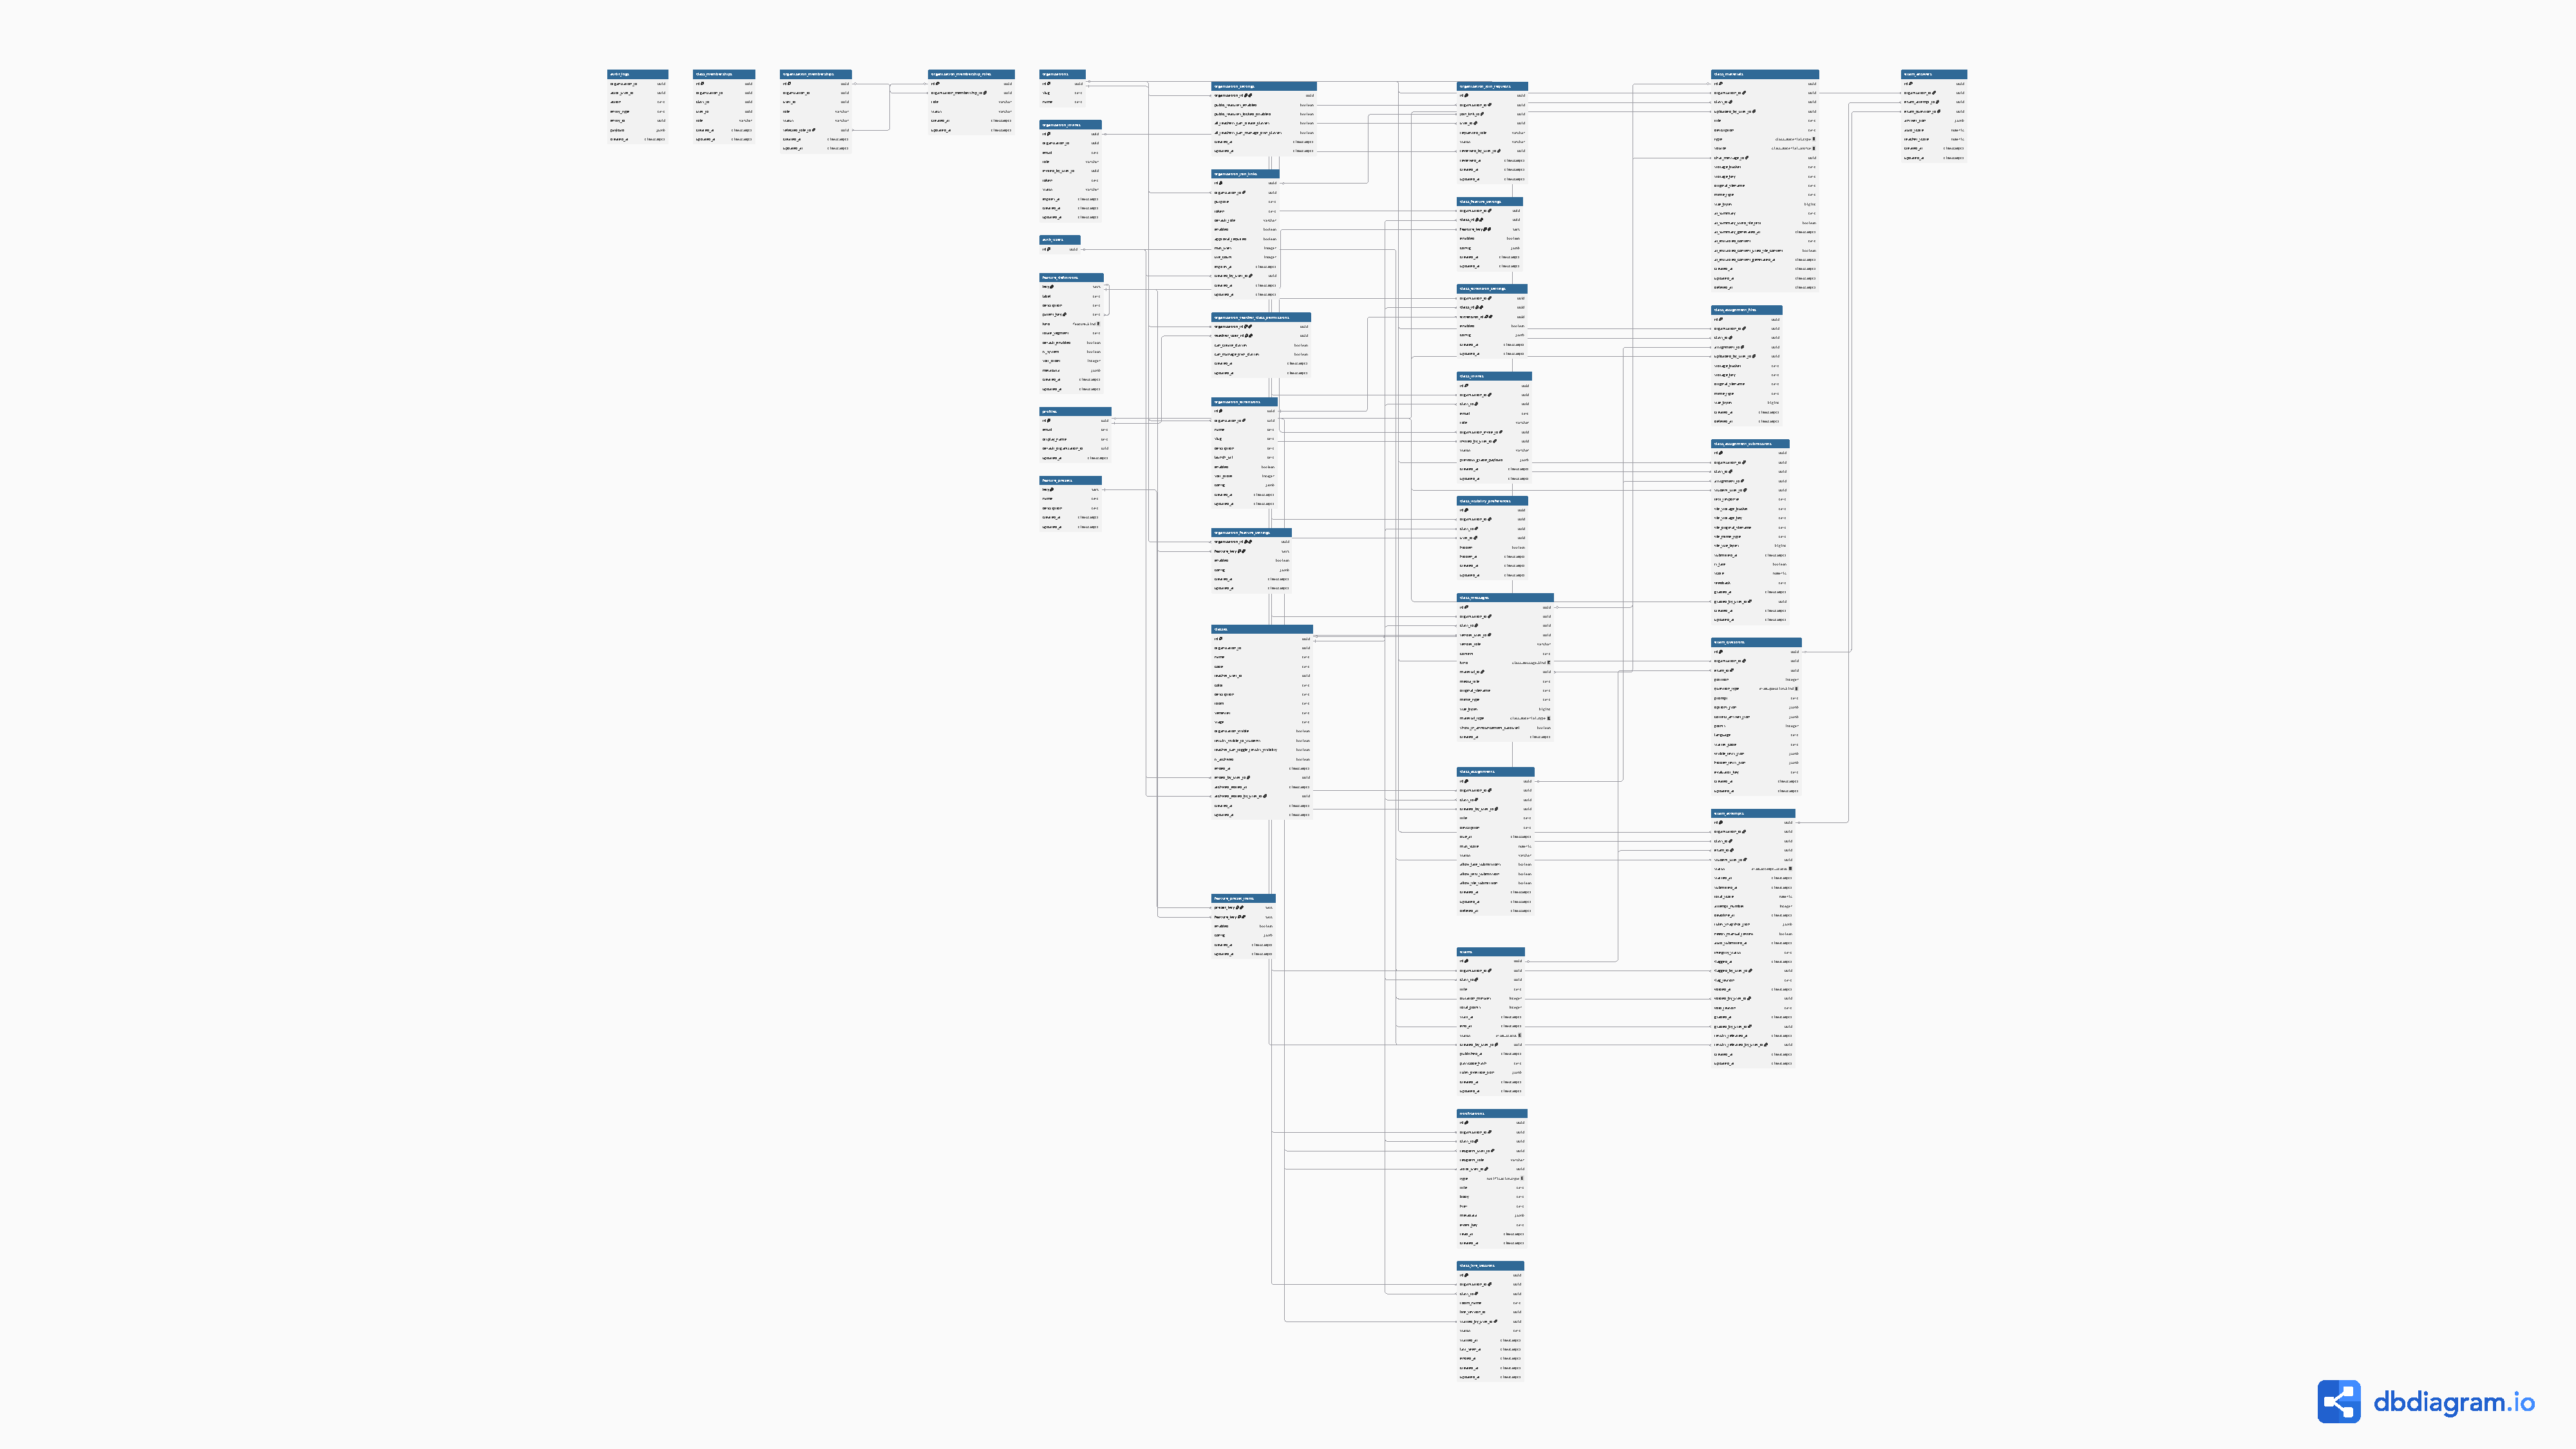
\includegraphics[
    page=1,
    angle=0,
    trim=580 25 580 25,
    clip,
    width=0.97\textwidth,
    height=0.93\textheight,
    keepaspectratio
  ]{figures/chapter5/database-erd.pdf}
  \caption{Entity Relationship Diagram of the EduVerse Database}
  \label{fig:eduverse_database_erd}
\end{figure}

\clearpage

\subsection{Principal Schema Groups}\label{subsec:principal_schema_groups}

The relational model is organized into several schema groups that correspond
to the main institutional and academic responsibilities of EduVerse. The
following overview introduces the principal table groups and their design
purpose before the detailed physical schema documentation.

\begingroup
\footnotesize
\renewcommand{\arraystretch}{1.16}
\setlength{\tabcolsep}{3pt}
\begin{longtable}{|L{0.18\textwidth}|L{0.35\textwidth}|L{0.39\textwidth}|}
  \caption{Principal Schema Groups in EduVerse}
  \label{tab:principal_schema_groups} \\
  \hline
  \textbf{Schema Group} & \textbf{Principal Tables} & \textbf{Design Purpose} \\
  \hline
  \endfirsthead
  \hline
  \textbf{Schema Group} & \textbf{Principal Tables} & \textbf{Design Purpose} \\
  \hline
  \endhead
  \hline
  \multicolumn{3}{r}{\small\textit{Continued on the next page}} \\
  \endfoot
  \hline
  \endlastfoot

  Core Organization and Identity &
  \db{organizations}, \db{profiles}, \db{organization_memberships},
  \db{organization_membership_roles} &
  Represents institutional workspaces, user identity context, organization
  membership, and role relationships. \\
  \hline

  Organization Access and Governance &
  \db{organization_invites}, \db{organization_settings},
  \db{organization_teacher_class_permissions}, \db{organization_join_links},
  \db{organization_join_requests} &
  Supports controlled membership entry, administrative settings, teacher
  permissions, and organization-level access governance. \\
  \hline

  Classes and Participation &
  \db{classes}, \db{class_memberships}, \db{class_visibility_preferences},
  \db{class_invites} &
  Represents class workspaces, participation, visibility, membership, and class
  lifecycle relationships. \\
  \hline

  Features and Extensions &
  \db{feature_definitions}, \db{feature_presets},
  \db{feature_preset_items}, \db{organization_feature_settings},
  \db{class_feature_settings}, \db{organization_extensions},
  \db{class_extension_settings} &
  Represents configurable platform capabilities and their organization- or
  class-level availability. \\
  \hline

  Materials and Communication &
  \db{class_materials}, \db{class_messages}, \db{notifications} &
  Supports class learning resources, communication, announcements, and user
  notification records. \\
  \hline

  Assignments and Submissions &
  \db{class_assignments}, \db{class_assignment_files},
  \db{class_assignment_submissions} &
  Represents assignment authoring, attached resources, student submission,
  grading, and feedback relationships. \\
  \hline

  Examinations &
  \db{exams}, \db{exam_questions}, \db{exam_attempts}, \db{exam_answers} &
  Represents examination definition, questions, student attempts, answers,
  grading, and assessment-state relationships. \\
  \hline

  Live Learning &
  \db{class_live_sessions} &
  Represents the lifecycle and class association of synchronous learning
  sessions. \\
  \hline

  System Audit &
  \db{audit_logs} &
  Represents recorded platform actions used for governance, traceability, and
  workflow history. \\
\end{longtable}
\endgroup

\subsection{Physical Schema Tables}
\label{subsec:database_tables}

The following tables document the principal columns, data types, keys, and
relationships of the EduVerse database. Table and column names are preserved
exactly as they appear in the documented schema.

\subsubsection*{Core Multi-Organization and User Model}

\EduSchemaTableStart{organizations}
\EduSchemaRow{id}{\db{uuid}}{PK.}
\EduSchemaRow{slug}{\db{text}}{Organization slug.}
\EduSchemaRow{name}{\db{text}}{Organization display name.}
\EduSchemaTableEnd

\EduSchemaTableStart{profiles}
\EduSchemaRow{id}{\db{uuid}}{PK; aligned with \db{auth.users.id} in the identity model.}
\EduSchemaRow{email}{\db{text}}{Profile email address.}
\EduSchemaRow{display_name}{\db{text}}{Visible user name.}
\EduSchemaRow{default_organization_id}{\db{uuid}}{Related to \db{organizations.id}.}
\EduSchemaRow{updated_at}{\db{timestamp}}{Profile update timestamp.}
\EduSchemaTableEnd

\subsubsection*{Roles, Memberships, Invitations, and Public Join Access}

\EduSchemaTableStart{organization_memberships}
\EduSchemaRow{id}{\db{uuid}}{PK.}
\EduSchemaRow{organization_id}{\db{uuid}}{Related to \db{organizations.id}.}
\EduSchemaRow{user_id}{\db{uuid}}{Related to the profile or authentication identity.}
\EduSchemaRow{role}{\db{public.app_role}}{Role enum.}
\EduSchemaRow{status}{\db{public.membership_status}}{Membership status enum.}
\EduSchemaRow{selected_role_id}{\db{uuid}}{\db{FK to organization_membership_roles.id}.}
\EduSchemaRow{created_at}{\db{timestamp}}{Creation timestamp.}
\EduSchemaRow{updated_at}{\db{timestamp}}{Update timestamp.}
\EduSchemaTableEnd

\EduSchemaTableStart{organization_membership_roles}
\EduSchemaRow{id}{\db{uuid}}{PK.}
\EduSchemaRow{organization_membership_id}{\db{uuid}}{\db{FK to organization_memberships.id}.}
\EduSchemaRow{role}{\db{public.app_role}}{Role enum.}
\EduSchemaRow{status}{\db{public.membership_status}}{Membership status enum.}
\EduSchemaRow{created_at}{\db{timestamp}}{Creation timestamp.}
\EduSchemaRow{updated_at}{\db{timestamp}}{Update timestamp.}
\EduSchemaTableEnd

\EduSchemaTableStart{organization_invites}
\EduSchemaRow{id}{\db{uuid}}{PK.}
\EduSchemaRow{organization_id}{\db{uuid}}{Related to \db{organizations.id}.}
\EduSchemaRow{email}{\db{text}}{Invite target email.}
\EduSchemaRow{role}{\db{public.app_role}}{Role enum.}
\EduSchemaRow{invited_by_user_id}{\db{uuid}}{Related to \db{auth.users.id}.}
\EduSchemaRow{token}{\db{text}}{Invite token.}
\EduSchemaRow{status}{\db{text}}{Invitation-status field used in the organization invite workflow.}
\EduSchemaRow{expires_at}{\db{timestamp}}{Invite expiry timestamp.}
\EduSchemaRow{created_at}{\db{timestamp}}{Creation timestamp.}
\EduSchemaRow{updated_at}{\db{timestamp}}{Update timestamp.}
\EduSchemaTableEnd

\EduSchemaTableStart{organization_settings}
\EduSchemaRow{organization_id}{\db{uuid}}{PK; \db{FK to organizations.id}.}
\EduSchemaRow{public_features_enabled}{\db{boolean}}{Public-feature availability flag.}
\EduSchemaRow{public_features_locked_disabled}{\db{boolean}}{Preset lock flag for disabled public features.}
\EduSchemaRow{all_teachers_can_create_classes}{\db{boolean}}{Teacher class-creation permission flag.}
\EduSchemaRow{all_teachers_can_manage_own_classes}{\db{boolean}}{Teacher class self-management permission flag.}
\EduSchemaRow{created_at}{\db{timestamp}}{Creation timestamp.}
\EduSchemaRow{updated_at}{\db{timestamp}}{Update timestamp.}
\EduSchemaTableEnd

\EduSchemaTableStart{organization_teacher_class_permissions}
\EduSchemaRow{organization_id}{\db{uuid}}{Composite PK; \db{FK to organizations.id}.}
\EduSchemaRow{teacher_user_id}{\db{uuid}}{Composite PK; \db{FK to profiles.id}.}
\EduSchemaRow{can_create_classes}{\db{boolean}}{Teacher override flag for class creation.}
\EduSchemaRow{can_manage_own_classes}{\db{boolean}}{Teacher override flag for managing owned classes.}
\EduSchemaRow{created_at}{\db{timestamp}}{Creation timestamp.}
\EduSchemaRow{updated_at}{\db{timestamp}}{Update timestamp.}
\EduSchemaTableEnd

\EduSchemaTableStart{organization_join_links}
\EduSchemaRow{id}{\db{uuid}}{PK.}
\EduSchemaRow{organization_id}{\db{uuid}}{\db{FK to organizations.id}.}
\EduSchemaRow{purpose}{\db{text}}{Join-link purpose descriptor.}
\EduSchemaRow{token}{\db{text}}{Join token.}
\EduSchemaRow{default_role}{\db{public.app_role}}{Default role enum, constrained to teacher or student.}
\EduSchemaRow{enabled}{\db{boolean}}{Link availability flag.}
\EduSchemaRow{approval_required}{\db{boolean}}{Approval workflow flag.}
\EduSchemaRow{max_uses}{\db{integer}}{Optional usage limit.}
\EduSchemaRow{use_count}{\db{integer}}{Current usage counter.}
\EduSchemaRow{expires_at}{\db{timestamp}}{Link expiry timestamp.}
\EduSchemaRow{created_by_user_id}{\db{uuid}}{\db{FK to auth.users.id}.}
\EduSchemaRow{created_at}{\db{timestamp}}{Creation timestamp.}
\EduSchemaRow{updated_at}{\db{timestamp}}{Update timestamp.}
\EduSchemaTableEnd

\EduSchemaTableStart{organization_join_requests}
\EduSchemaRow{id}{\db{uuid}}{PK.}
\EduSchemaRow{organization_id}{\db{uuid}}{\db{FK to organizations.id}.}
\EduSchemaRow{join_link_id}{\db{uuid}}{\db{FK to organization_join_links.id}.}
\EduSchemaRow{user_id}{\db{uuid}}{\db{FK to auth.users.id}.}
\EduSchemaRow{requested_role}{\db{public.app_role}}{Requested role enum.}
\EduSchemaRow{status}{\db{text}}{Status text; current values include \db{pending}, \db{approved}, and \db{rejected}.}
\EduSchemaRow{reviewed_by_user_id}{\db{uuid}}{\db{FK to auth.users.id}.}
\EduSchemaRow{reviewed_at}{\db{timestamp}}{Review timestamp.}
\EduSchemaRow{created_at}{\db{timestamp}}{Creation timestamp.}
\EduSchemaRow{updated_at}{\db{timestamp}}{Update timestamp.}
\EduSchemaTableEnd

\EduSchemaTableStart{class_invites}
\EduSchemaRow{id}{\db{uuid}}{PK.}
\EduSchemaRow{organization_id}{\db{uuid}}{\db{FK to organizations.id}.}
\EduSchemaRow{class_id}{\db{uuid}}{\db{FK to classes.id}.}
\EduSchemaRow{email}{\db{text}}{Invite target email.}
\EduSchemaRow{role}{\db{public.class_membership_role}}{Class membership role enum.}
\EduSchemaRow{organization_invite_id}{\db{uuid}}{\db{FK to organization_invites.id}.}
\EduSchemaRow{invited_by_user_id}{\db{uuid}}{\db{FK to auth.users.id}.}
\EduSchemaRow{status}{\db{public.membership_status}}{Membership status enum.}
\EduSchemaRow{previous_grade_payload}{\db{json/jsonb}}{Imported previous-term grade payload.}
\EduSchemaRow{created_at}{\db{timestamp}}{Creation timestamp.}
\EduSchemaRow{updated_at}{\db{timestamp}}{Update timestamp.}
\EduSchemaTableEnd

\subsubsection*{Classes and Class Visibility}

\EduSchemaTableStart{classes}
\EduSchemaRow{id}{\db{uuid}}{PK.}
\EduSchemaRow{organization_id}{\db{uuid}}{Related to \db{organizations.id}.}
\EduSchemaRow{name}{\db{text}}{Class name.}
\EduSchemaRow{code}{\db{text}}{Class code.}
\EduSchemaRow{teacher_user_id}{\db{uuid}}{Related to \db{profiles.id}.}
\EduSchemaRow{color}{\db{text}}{Class color identifier.}
\EduSchemaRow{description}{\db{text}}{Class description.}
\EduSchemaRow{room}{\db{text}}{Room or location field.}
\EduSchemaRow{semester}{\db{text}}{Required semester text.}
\EduSchemaRow{stage}{\db{text}}{Required stage text.}
\EduSchemaRow{organization_visible}{\db{boolean}}{Organization-wide visibility flag.}
\EduSchemaRow{results_visible_to_students}{\db{boolean}}{Student results visibility flag.}
\EduSchemaRow{teacher_can_toggle_results_visibility}{\db{boolean}}{Teacher permission flag for results visibility.}
\EduSchemaRow{is_archived}{\db{boolean}}{Archive lifecycle flag.}
\EduSchemaRow{ended_at}{\db{timestamp}}{Class end timestamp.}
\EduSchemaRow{ended_by_user_id}{\db{uuid}}{\db{FK to auth.users.id}.}
\EduSchemaRow{archived_edited_at}{\db{timestamp}}{Archived-state edit timestamp.}
\EduSchemaRow{archived_edited_by_user_id}{\db{uuid}}{\db{FK to auth.users.id}.}
\EduSchemaRow{created_at}{\db{timestamp}}{Creation timestamp.}
\EduSchemaRow{updated_at}{\db{timestamp}}{Update timestamp.}
\EduSchemaTableEnd

\EduSchemaTableStart{class_memberships}
\EduSchemaRow{id}{\db{uuid}}{PK.}
\EduSchemaRow{organization_id}{\db{uuid}}{Related to \db{organizations.id}.}
\EduSchemaRow{class_id}{\db{uuid}}{Related to \db{classes.id}.}
\EduSchemaRow{user_id}{\db{uuid}}{Related to the profile or authentication identity.}
\EduSchemaRow{role}{\db{text}}{Class-level role field; current values include \db{teacher}, \db{student}, and \db{ta}.}
\EduSchemaRow{created_at}{\db{timestamp}}{Creation timestamp.}
\EduSchemaRow{updated_at}{\db{timestamp}}{Update timestamp.}
\EduSchemaTableEnd

\EduSchemaTableStart{class_visibility_preferences}
\EduSchemaRow{id}{\db{uuid}}{PK.}
\EduSchemaRow{organization_id}{\db{uuid}}{\db{FK to organizations.id}.}
\EduSchemaRow{class_id}{\db{uuid}}{\db{FK to classes.id}.}
\EduSchemaRow{user_id}{\db{uuid}}{\db{FK to auth.users.id}.}
\EduSchemaRow{hidden}{\db{boolean}}{Student hide or show flag.}
\EduSchemaRow{hidden_at}{\db{timestamp}}{Hide timestamp.}
\EduSchemaRow{created_at}{\db{timestamp}}{Creation timestamp.}
\EduSchemaRow{updated_at}{\db{timestamp}}{Update timestamp.}
\EduSchemaTableEnd

\EduNeedspace{10\baselineskip}
\subsubsection*{Feature Flags and Extensions}

\EduSchemaTableStart{feature_definitions}
\EduSchemaRow{key}{\db{text}}{PK.}
\EduSchemaRow{label}{\db{text}}{Feature label.}
\EduSchemaRow{description}{\db{text}}{Feature description.}
\EduSchemaRow{parent_key}{\db{text}}{\db{FK to feature_definitions.key}.}
\EduSchemaRow{kind}{\db{public.feature_kind}}{Feature kind enum.}
\EduSchemaRow{route_segment}{\db{text}}{Navigation route segment.}
\EduSchemaRow{default_enabled}{\db{boolean}}{Default enablement flag.}
\EduSchemaRow{is_system}{\db{boolean}}{System-managed feature flag.}
\EduSchemaRow{sort_order}{\db{integer}}{Display ordering value.}
\EduSchemaRow{metadata}{\db{json/jsonb}}{Feature metadata payload.}
\EduSchemaRow{created_at}{\db{timestamp}}{Creation timestamp.}
\EduSchemaRow{updated_at}{\db{timestamp}}{Update timestamp.}
\EduSchemaTableEnd

\EduSchemaTableStart{feature_presets}
\EduSchemaRow{key}{\db{text}}{PK.}
\EduSchemaRow{name}{\db{text}}{Preset name.}
\EduSchemaRow{description}{\db{text}}{Preset description.}
\EduSchemaRow{created_at}{\db{timestamp}}{Creation timestamp.}
\EduSchemaRow{updated_at}{\db{timestamp}}{Update timestamp.}
\EduSchemaTableEnd

\EduSchemaTableStart{feature_preset_items}
\EduSchemaRow{preset_key}{\db{text}}{Composite PK; \db{FK to feature_presets.key}.}
\EduSchemaRow{feature_key}{\db{text}}{Composite PK; \db{FK to feature_definitions.key}.}
\EduSchemaRow{enabled}{\db{boolean}}{Preset enablement flag.}
\EduSchemaRow{config}{\db{json/jsonb}}{Preset configuration payload.}
\EduSchemaRow{created_at}{\db{timestamp}}{Creation timestamp.}
\EduSchemaRow{updated_at}{\db{timestamp}}{Update timestamp.}
\EduSchemaTableEnd

\EduSchemaTableStart{organization_feature_settings}
\EduSchemaRow{organization_id}{\db{uuid}}{Composite PK; \db{FK to organizations.id}.}
\EduSchemaRow{feature_key}{\db{text}}{Composite PK; \db{FK to feature_definitions.key}.}
\EduSchemaRow{enabled}{\db{boolean}}{Organization-level feature flag.}
\EduSchemaRow{config}{\db{json/jsonb}}{Configuration payload; may store lock metadata.}
\EduSchemaRow{created_at}{\db{timestamp}}{Creation timestamp.}
\EduSchemaRow{updated_at}{\db{timestamp}}{Update timestamp.}
\EduSchemaTableEnd

\EduSchemaTableStart{class_feature_settings}
\EduSchemaRow{organization_id}{\db{uuid}}{\db{FK to organizations.id}.}
\EduSchemaRow{class_id}{\db{uuid}}{Composite PK; \db{FK to classes.id}.}
\EduSchemaRow{feature_key}{\db{text}}{Composite PK; \db{FK to feature_definitions.key}.}
\EduSchemaRow{enabled}{\db{boolean}}{Class-level feature flag.}
\EduSchemaRow{config}{\db{json/jsonb}}{Class configuration payload.}
\EduSchemaRow{created_at}{\db{timestamp}}{Creation timestamp.}
\EduSchemaRow{updated_at}{\db{timestamp}}{Update timestamp.}
\EduSchemaTableEnd

\EduSchemaTableStart{organization_extensions}
\EduSchemaRow{id}{\db{uuid}}{PK.}
\EduSchemaRow{organization_id}{\db{uuid}}{\db{FK to organizations.id}.}
\EduSchemaRow{name}{\db{text}}{Extension name.}
\EduSchemaRow{slug}{\db{text}}{Extension slug.}
\EduSchemaRow{description}{\db{text}}{Extension description.}
\EduSchemaRow{launch_url}{\db{text}}{Extension launch URL.}
\EduSchemaRow{enabled}{\db{boolean}}{Extension enablement flag.}
\EduSchemaRow{sort_order}{\db{integer}}{Display ordering value.}
\EduSchemaRow{config}{\db{json/jsonb}}{Extension configuration payload.}
\EduSchemaRow{created_at}{\db{timestamp}}{Creation timestamp.}
\EduSchemaRow{updated_at}{\db{timestamp}}{Update timestamp.}
\EduSchemaTableEnd

\EduSchemaTableStart{class_extension_settings}
\EduSchemaRow{organization_id}{\db{uuid}}{\db{FK to organizations.id}.}
\EduSchemaRow{class_id}{\db{uuid}}{Composite PK; \db{FK to classes.id}.}
\EduSchemaRow{extension_id}{\db{uuid}}{Composite PK; \db{FK to organization_extensions.id}.}
\EduSchemaRow{enabled}{\db{boolean}}{Class-level extension enablement flag.}
\EduSchemaRow{config}{\db{json/jsonb}}{Class-level extension configuration payload.}
\EduSchemaRow{created_at}{\db{timestamp}}{Creation timestamp.}
\EduSchemaRow{updated_at}{\db{timestamp}}{Update timestamp.}
\EduSchemaTableEnd

\subsubsection*{Materials, Chat, and Announcements}

\EduSchemaTableStart{class_materials}
\EduSchemaRow{id}{\db{uuid}}{PK.}
\EduSchemaRow{organization_id}{\db{uuid}}{\db{FK to organizations.id}.}
\EduSchemaRow{class_id}{\db{uuid}}{\db{FK to classes.id}.}
\EduSchemaRow{uploaded_by_user_id}{\db{uuid}}{\db{FK to profiles.id}.}
\EduSchemaRow{title}{\db{text}}{Material title.}
\EduSchemaRow{description}{\db{text}}{Material description.}
\EduSchemaRow{type}{\db{public.class_material_type}}{Material type enum.}
\EduSchemaRow{source}{\db{public.class_material_source}}{Source enum.}
\EduSchemaRow{chat_message_id}{\db{uuid}}{\db{FK to class_messages.id}.}
\EduSchemaRow{storage_bucket}{\db{text}}{AWS S3 bucket reference.}
\EduSchemaRow{storage_key}{\db{text}}{AWS S3 object key reference.}
\EduSchemaRow{original_filename}{\db{text}}{Original uploaded file name.}
\EduSchemaRow{mime_type}{\db{text}}{Uploaded file MIME type.}
\EduSchemaRow{size_bytes}{\db{integer}}{Stored file size.}
\EduSchemaRow{ai_summary}{\db{text}}{Cached AI summary text.}
\EduSchemaRow{ai_summary_used_file_text}{\db{boolean}}{Flag indicating whether file text was used to generate the cached AI summary.}
\EduSchemaRow{ai_summary_generated_at}{\db{timestamp}}{AI summary generation timestamp.}
\EduSchemaRow{ai_extracted_content}{\db{text}}{Cached extracted-content field.}
\EduSchemaRow{ai_extracted_content_used_file_content}{\db{boolean}}{Flag indicating whether file content was used for cached extraction.}
\EduSchemaRow{ai_extracted_content_generated_at}{\db{timestamp}}{Extracted-content generation timestamp.}
\EduSchemaRow{deleted_at}{\db{timestamp}}{Soft-delete timestamp.}
\EduSchemaRow{created_at}{\db{timestamp}}{Creation timestamp.}
\EduSchemaRow{updated_at}{\db{timestamp}}{Update timestamp.}
\EduSchemaTableEnd

\EduSchemaTableStart{class_messages}
\EduSchemaRow{id}{\db{uuid}}{PK.}
\EduSchemaRow{organization_id}{\db{uuid}}{\db{FK to organizations.id}.}
\EduSchemaRow{class_id}{\db{uuid}}{\db{FK to classes.id}.}
\EduSchemaRow{sender_user_id}{\db{uuid}}{\db{FK to profiles.id}.}
\EduSchemaRow{sender_role}{\db{text}}{Checked text role field; current values include \db{student}, \db{teacher}, and \db{admin}.}
\EduSchemaRow{content}{\db{text}}{Message body text.}
\EduSchemaRow{kind}{\db{public.class_message_kind}}{Message kind enum; announcements are represented by rows where \db{kind = 'announcement'}.}
\EduSchemaRow{material_id}{\db{uuid}}{\db{FK to class_materials.id}.}
\EduSchemaRow{media_title}{\db{text}}{Chat-media title field.}
\EduSchemaRow{original_filename}{\db{text}}{Original media file name.}
\EduSchemaRow{mime_type}{\db{text}}{Media MIME type.}
\EduSchemaRow{size_bytes}{\db{integer}}{Stored media size.}
\EduSchemaRow{material_type}{\db{text}}{Chat-media material descriptor used for uploaded class content.}
\EduSchemaRow{show_in_announcement_carousel}{\db{boolean}}{Announcement carousel display flag.}
\EduSchemaRow{created_at}{\db{timestamp}}{Creation timestamp.}
\EduSchemaTableEnd

\subsubsection*{Assignments and Submissions}

\EduSchemaTableStart{class_assignments}
\EduSchemaRow{id}{\db{uuid}}{PK.}
\EduSchemaRow{organization_id}{\db{uuid}}{\db{FK to organizations.id}.}
\EduSchemaRow{class_id}{\db{uuid}}{\db{FK to classes.id}.}
\EduSchemaRow{created_by_user_id}{\db{uuid}}{\db{FK to profiles.id}.}
\EduSchemaRow{title}{\db{text}}{Assignment title.}
\EduSchemaRow{description}{\db{text}}{Assignment description.}
\EduSchemaRow{due_at}{\db{timestamp}}{Submission due timestamp.}
\EduSchemaRow{max_score}{\db{numeric}}{Maximum assignment score.}
\EduSchemaRow{status}{\db{text}}{Status text; current values include \db{draft} and \db{published}.}
\EduSchemaRow{allow_late_submissions}{\db{boolean}}{Late-submission policy flag.}
\EduSchemaRow{allow_text_submission}{\db{boolean}}{Text-submission policy flag.}
\EduSchemaRow{allow_file_submission}{\db{boolean}}{File-submission policy flag.}
\EduSchemaRow{created_at}{\db{timestamp}}{Creation timestamp.}
\EduSchemaRow{updated_at}{\db{timestamp}}{Update timestamp.}
\EduSchemaRow{deleted_at}{\db{timestamp}}{Soft-delete timestamp.}
\EduSchemaTableEnd

\EduSchemaTableStart{class_assignment_files}
\EduSchemaRow{id}{\db{uuid}}{PK.}
\EduSchemaRow{organization_id}{\db{uuid}}{\db{FK to organizations.id}.}
\EduSchemaRow{class_id}{\db{uuid}}{\db{FK to classes.id}.}
\EduSchemaRow{assignment_id}{\db{uuid}}{\db{FK to class_assignments.id}.}
\EduSchemaRow{uploaded_by_user_id}{\db{uuid}}{\db{FK to profiles.id}.}
\EduSchemaRow{storage_bucket}{\db{text}}{AWS S3 bucket reference.}
\EduSchemaRow{storage_key}{\db{text}}{AWS S3 object key reference.}
\EduSchemaRow{original_filename}{\db{text}}{Original attachment file name.}
\EduSchemaRow{mime_type}{\db{text}}{Attachment MIME type.}
\EduSchemaRow{size_bytes}{\db{integer}}{Attachment size.}
\EduSchemaRow{created_at}{\db{timestamp}}{Creation timestamp.}
\EduSchemaRow{deleted_at}{\db{timestamp}}{Soft-delete timestamp.}
\EduSchemaTableEnd

\EduSchemaTableStart{class_assignment_submissions}
\EduSchemaRow{id}{\db{uuid}}{PK.}
\EduSchemaRow{organization_id}{\db{uuid}}{\db{FK to organizations.id}.}
\EduSchemaRow{class_id}{\db{uuid}}{\db{FK to classes.id}.}
\EduSchemaRow{assignment_id}{\db{uuid}}{\db{FK to class_assignments.id}.}
\EduSchemaRow{student_user_id}{\db{uuid}}{\db{FK to profiles.id}.}
\EduSchemaRow{text_response}{\db{text}}{Text submission body.}
\EduSchemaRow{file_storage_bucket}{\db{text}}{AWS S3 bucket reference for submitted files.}
\EduSchemaRow{file_storage_key}{\db{text}}{AWS S3 object key reference for submitted files.}
\EduSchemaRow{file_original_filename}{\db{text}}{Original submitted file name.}
\EduSchemaRow{file_mime_type}{\db{text}}{Submitted file MIME type.}
\EduSchemaRow{file_size_bytes}{\db{integer}}{Submitted file size.}
\EduSchemaRow{submitted_at}{\db{timestamp}}{Submission timestamp.}
\EduSchemaRow{is_late}{\db{boolean}}{Late-submission flag.}
\EduSchemaRow{score}{\db{numeric}}{Recorded assignment score.}
\EduSchemaRow{feedback}{\db{text}}{Grading feedback.}
\EduSchemaRow{graded_at}{\db{timestamp}}{Grading timestamp.}
\EduSchemaRow{graded_by_user_id}{\db{uuid}}{\db{FK to profiles.id}.}
\EduSchemaRow{created_at}{\db{timestamp}}{Creation timestamp.}
\EduSchemaRow{updated_at}{\db{timestamp}}{Update timestamp.}
\EduSchemaTableEnd

\EduNeedspace{10\baselineskip}
\subsubsection*{Exams, Attempts, Answers, and Results}

\EduSchemaTableStart{exams}
\EduSchemaRow{id}{\db{uuid}}{PK.}
\EduSchemaRow{organization_id}{\db{uuid}}{\db{FK to organizations.id}.}
\EduSchemaRow{class_id}{\db{uuid}}{\db{FK to classes.id}.}
\EduSchemaRow{title}{\db{text}}{Exam title.}
\EduSchemaRow{duration_minutes}{\db{integer}}{Configured exam duration.}
\EduSchemaRow{total_points}{\db{numeric}}{Total exam points.}
\EduSchemaRow{start_at}{\db{timestamp}}{Exam start timestamp.}
\EduSchemaRow{end_at}{\db{timestamp}}{Exam end timestamp.}
\EduSchemaRow{status}{\db{public.exam_status}}{Exam status enum.}
\EduSchemaRow{created_by_user_id}{\db{uuid}}{\db{FK to auth.users.id}.}
\EduSchemaRow{published_at}{\db{timestamp}}{Publish timestamp.}
\EduSchemaRow{passcode_hash}{\db{text}}{Optional stored passcode hash.}
\EduSchemaRow{rules_override_json}{\db{json/jsonb}}{Exam rules override payload.}
\EduSchemaRow{created_at}{\db{timestamp}}{Creation timestamp.}
\EduSchemaRow{updated_at}{\db{timestamp}}{Update timestamp.}
\EduSchemaTableEnd

\EduSchemaTableStart{exam_questions}
\EduSchemaRow{id}{\db{uuid}}{PK.}
\EduSchemaRow{organization_id}{\db{uuid}}{\db{FK to organizations.id}.}
\EduSchemaRow{exam_id}{\db{uuid}}{\db{FK to exams.id}.}
\EduSchemaRow{position}{\db{integer}}{Question ordering value.}
\EduSchemaRow{question_type}{\db{public.exam_question_kind}}{Question type enum.}
\EduSchemaRow{prompt}{\db{text}}{Question prompt text.}
\EduSchemaRow{options_json}{\db{json/jsonb}}{Structured option payload.}
\EduSchemaRow{correct_answer_json}{\db{json/jsonb}}{Structured correct-answer payload.}
\EduSchemaRow{points}{\db{numeric}}{Question score value.}
\EduSchemaRow{language}{\db{text}}{Question language marker.}
\EduSchemaRow{starter_code}{\db{text}}{Starter code text for coding questions.}
\EduSchemaRow{visible_tests_json}{\db{json/jsonb}}{Visible test payload.}
\EduSchemaRow{hidden_tests_json}{\db{json/jsonb}}{Hidden test payload.}
\EduSchemaRow{evaluator_key}{\db{text}}{Evaluator identifier.}
\EduSchemaRow{created_at}{\db{timestamp}}{Creation timestamp.}
\EduSchemaRow{updated_at}{\db{timestamp}}{Update timestamp.}
\EduSchemaTableEnd

\EduSchemaTableStart{exam_attempts}
\EduSchemaRow{id}{\db{uuid}}{PK.}
\EduSchemaRow{organization_id}{\db{uuid}}{\db{FK to organizations.id}.}
\EduSchemaRow{class_id}{\db{uuid}}{\db{FK to classes.id}.}
\EduSchemaRow{exam_id}{\db{uuid}}{\db{FK to exams.id}.}
\EduSchemaRow{student_user_id}{\db{uuid}}{\db{FK to auth.users.id}.}
\EduSchemaRow{status}{\db{public.exam_attempt_status}}{Attempt status enum.}
\EduSchemaRow{started_at}{\db{timestamp}}{Attempt start timestamp.}
\EduSchemaRow{submitted_at}{\db{timestamp}}{Attempt submission timestamp.}
\EduSchemaRow{total_score}{\db{numeric}}{Stores the exam-level result directly.}
\EduSchemaRow{attempt_number}{\db{integer}}{Retake or attempt counter.}
\EduSchemaRow{deadline_at}{\db{timestamp}}{Effective attempt deadline.}
\EduSchemaRow{rules_snapshot_json}{\db{json/jsonb}}{Applied rules snapshot payload.}
\EduSchemaRow{needs_manual_review}{\db{boolean}}{Manual-review flag.}
\EduSchemaRow{auto_submitted_at}{\db{timestamp}}{Automatic submission timestamp.}
\EduSchemaRow{integrity_status}{\db{text}}{Integrity status text; current values include \db{clear}, \db{reported}, \db{flagged}, and \db{voided}.}
\EduSchemaRow{flagged_at}{\db{timestamp}}{Integrity flag timestamp.}
\EduSchemaRow{flagged_by_user_id}{\db{uuid}}{\db{FK to auth.users.id}.}
\EduSchemaRow{flag_reason}{\db{text}}{Integrity flag reason.}
\EduSchemaRow{voided_at}{\db{timestamp}}{Void timestamp.}
\EduSchemaRow{voided_by_user_id}{\db{uuid}}{\db{FK to auth.users.id}.}
\EduSchemaRow{void_reason}{\db{text}}{Void reason.}
\EduSchemaRow{graded_at}{\db{timestamp}}{Grading timestamp.}
\EduSchemaRow{graded_by_user_id}{\db{uuid}}{\db{FK to auth.users.id}.}
\EduSchemaRow{results_released_at}{\db{timestamp}}{Results-release timestamp.}
\EduSchemaRow{results_released_by_user_id}{\db{uuid}}{\db{FK to auth.users.id}.}
\EduSchemaRow{created_at}{\db{timestamp}}{Creation timestamp.}
\EduSchemaRow{updated_at}{\db{timestamp}}{Update timestamp.}
\EduSchemaTableEnd

\EduSchemaTableStart{exam_answers}
\EduSchemaRow{id}{\db{uuid}}{PK.}
\EduSchemaRow{organization_id}{\db{uuid}}{\db{FK to organizations.id}.}
\EduSchemaRow{exam_attempt_id}{\db{uuid}}{\db{FK to exam_attempts.id}.}
\EduSchemaRow{exam_question_id}{\db{uuid}}{\db{FK to exam_questions.id}.}
\EduSchemaRow{answer_json}{\db{json/jsonb}}{Stored submitted answer payload.}
\EduSchemaRow{auto_score}{\db{numeric}}{Stores question-level auto-scoring directly.}
\EduSchemaRow{teacher_score}{\db{numeric}}{Stores question-level teacher scoring directly.}
\EduSchemaRow{created_at}{\db{timestamp}}{Creation timestamp.}
\EduSchemaRow{updated_at}{\db{timestamp}}{Update timestamp.}
\EduSchemaTableEnd

\subsubsection*{Notifications and Live Sessions}

\EduSchemaTableStart{notifications}
\EduSchemaRow{id}{\db{uuid}}{PK.}
\EduSchemaRow{organization_id}{\db{uuid}}{\db{FK to organizations.id}.}
\EduSchemaRow{class_id}{\db{uuid}}{\db{FK to classes.id}.}
\EduSchemaRow{recipient_user_id}{\db{uuid}}{\db{FK to profiles.id}.}
\EduSchemaRow{recipient_role}{\db{public.app_role}}{Role-scoped notification enum field.}
\EduSchemaRow{actor_user_id}{\db{uuid}}{\db{FK to profiles.id}.}
\EduSchemaRow{type}{\db{public.notification_type}}{Notification type enum.}
\EduSchemaRow{title}{\db{text}}{Notification title.}
\EduSchemaRow{body}{\db{text}}{Notification body text.}
\EduSchemaRow{href}{\db{text}}{Navigation target.}
\EduSchemaRow{metadata}{\db{json/jsonb}}{Notification metadata payload.}
\EduSchemaRow{event_key}{\db{text}}{Event deduplication or tracking key.}
\EduSchemaRow{read_at}{\db{timestamp}}{Read timestamp.}
\EduSchemaRow{created_at}{\db{timestamp}}{Creation timestamp.}
\EduSchemaTableEnd

\EduSchemaTableStart{class_live_sessions}
\EduSchemaRow{id}{\db{uuid}}{PK.}
\EduSchemaRow{organization_id}{\db{uuid}}{\db{FK to organizations.id}.}
\EduSchemaRow{class_id}{\db{uuid}}{\db{FK to classes.id}.}
\EduSchemaRow{room_name}{\db{text}}{Session room name.}
\EduSchemaRow{live_session_id}{\db{text}}{LiveKit-related session identifier.}
\EduSchemaRow{started_by_user_id}{\db{uuid}}{\db{FK to profiles.id}.}
\EduSchemaRow{status}{\db{text}}{Session status text; current values include \db{pending}, \db{live}, and \db{ended}.}
\EduSchemaRow{started_at}{\db{timestamp}}{Session start timestamp.}
\EduSchemaRow{last_seen_at}{\db{timestamp}}{Last heartbeat timestamp.}
\EduSchemaRow{ended_at}{\db{timestamp}}{Session end timestamp.}
\EduSchemaRow{created_at}{\db{timestamp}}{Creation timestamp.}
\EduSchemaRow{updated_at}{\db{timestamp}}{Update timestamp.}
\EduSchemaTableEnd

\subsubsection*{Audit Logs and External Authentication References}

\EduSchemaTableStart{audit_logs}
\EduSchemaRow{organization_id}{\db{uuid}}{Related to \db{organizations.id}.}
\EduSchemaRow{actor_user_id}{\db{uuid}}{Related to \db{auth.users.id}.}
\EduSchemaRow{action}{\db{text}}{Audit action key.}
\EduSchemaRow{entity_type}{\db{text}}{Polymorphic entity type discriminator.}
\EduSchemaRow{entity_id}{\db{reference}}{Polymorphic reference to related entity records.}
\EduSchemaRow{payload}{\db{json/jsonb}}{Audit payload.}
\EduSchemaRow{created_at}{\db{timestamp}}{Creation timestamp.}
\EduSchemaTableEnd

\EduSchemaTableStart{auth.users}
\EduSchemaRow{id}{\db{uuid}}{PK; external Supabase authentication user identifier.}
\EduSchemaNote{This external table is referenced by invite, join-link, join-request, exam, and class-lifecycle user fields in the EduVerse schema.}
\EduSchemaTableEnd


% Fallback barrier for builds that do not load placeins in the active preamble.

\newcommand{\EduUiFigure}[3]{%
  \begin{figure}[htbp]
    \centering
    \includegraphics[
      width=0.95\textwidth,
      height=0.82\textheight,
      keepaspectratio
    ]{#1}
    \caption{#2}
    \label{#3}
  \end{figure}
}

\section{Interface and Interaction Design}\label{sec:interface_and_interaction_design}

The EduVerse interface design reflects the role-aware and class-centered
structure established in the system model. Administrative, instructional, and
student-facing actions are presented through different workspace contexts
while maintaining consistent navigation and interaction patterns across the
platform.

The screenshots in this section show how these design principles appear in the
implemented web interface and demonstrate the resulting interaction design.

\subsection{Access and Identity Interfaces}

Access and identity interfaces establish the organization and role context used
throughout the platform. Their design separates account authentication from
workspace selection and personal account settings so that users who participate
in multiple contexts can move between them without changing account identity.

\EduUiFigure
  {figures/screenshots/1_Authentication Screen.png}
  {Authentication interface showing sign-in and sign-up forms for EduVerse users.}
  {fig:ui-auth-signin-signup}

\EduUiFigure
  {figures/screenshots/2-organization-and-active-role-selection-switcher.png}
  {Organization and active-role selector used to switch between available EduVerse workspaces.}
  {fig:ui-auth-organization-role-switcher}

\EduUiFigure
  {figures/screenshots/26_Profile and User Settings.png}
  {User profile and settings interface showing role context, theme preferences, and password management controls.}
  {fig:ui-profile-settings}

\clearpage

\subsection{Administrative Governance Interfaces}

Administrative interfaces group organization setup, membership,
permissions, class oversight, and feature configuration within a dedicated
governance context. This separation keeps institution-level controls distinct
from the day-to-day instructional activity that occurs inside classes.

The interface design also presents configurable options through structured
settings and management views rather than exposing the same controls to every
actor.

\EduUiFigure
  {figures/screenshots/10_Organization Creation and Initial Feature Availability.png}
  {Organization creation interface showing template-based setup and initial feature-availability controls for different educational contexts.}
  {fig:ui-admin-organization-creation}

\EduUiFigure
  {figures/screenshots/3_Administrator dashboard showing organization statistics and class management controls.png}
  {Organization administrator dashboard showing class oversight and organization-wide statistics.}
  {fig:ui-admin-dashboard}

\EduUiFigure
  {figures/screenshots/4_Class CreateEdit Settings Dialog.png}
  {Class creation and feature-configuration dialog used to define class properties and enabled tools.}
  {fig:ui-admin-class-settings}

\EduUiFigure
  {figures/screenshots/5_Past Terms (Admin interface).png}
  {Past-terms administration interface used to review archived classes and historical academic records.}
  {fig:ui-admin-past-terms}

\EduUiFigure
  {figures/screenshots/6_Organization Members and Invitations.png}
  {Organization members and invitations interface showing role assignment and invitation-management controls.}
  {fig:ui-admin-members}

\EduUiFigure
  {figures/screenshots/7_Public Join Links and Join Requests.png}
  {Public join-link management interface showing join-link creation and request-handling controls.}
  {fig:ui-admin-join-links}

\EduUiFigure
  {figures/screenshots/8_Public Join Page.png}
  {Public join page used by a student to request access to an organization workspace.}
  {fig:ui-admin-public-join}

\EduUiFigure
  {figures/screenshots/9_Organization Settings and Teacher Permissions.png}
  {Organization settings interface showing public-feature controls and teacher class-permission settings.}
  {fig:ui-admin-settings}

\clearpage

\subsection{Classroom and Learning Interfaces}

Classroom interfaces provide the primary day-to-day learning context for
Teachers and Students. Class navigation keeps learning resources,
communication, notifications, and other enabled tools associated with the same
academic workspace while presenting actions according to the current role.

\EduUiFigure
  {figures/screenshots/11-class-home-classroom-workspace.png}
  {Class home interface showing the main classroom workspace and available learning tools.}
  {fig:ui-class-home}

\EduUiFigure
  {figures/screenshots/12_Materials Library and Upload Controls (Teacher interface).png}
  {Classroom materials interface used to access uploaded learning resources and study actions.}
  {fig:ui-class-materials}

\EduUiFigure
  {figures/screenshots/14_Class Chat and Announcements.png}
  {Class chat and announcements interface supporting class-wide discussion and instructor notices.}
  {fig:ui-class-chat-announcements}

\EduUiFigure
  {figures/screenshots/15_Notifications Panel or Page.png}
  {Notifications panel showing alerts for live sessions, materials, examinations, and announcements.}
  {fig:ui-class-notifications}

\clearpage

\subsection{Assessment and Submission Interfaces}

Assessment interfaces separate authoring and review controls from student
participation surfaces. Teacher-facing views emphasize creation, configuration,
grading, and review, while student-facing views focus on the actions required
to complete and review permitted assessment tasks.

This role-oriented separation reduces interface complexity and prevents
administrative or authoring controls from appearing in student task flows.

\EduUiFigure
  {figures/screenshots/16_Assignment Management and Submission Review (Teacher interface).png}
  {Assignment management interface showing teacher-side assignment creation, submission review, and grading controls.}
  {fig:ui-assignment-management}

\EduUiFigure
  {figures/screenshots/17_Student Assignment Submission Screen.png}
  {Student assignment submission interface showing response entry and file-upload controls.}
  {fig:ui-assignment-submission}

\EduUiFigure
  {figures/screenshots/18_Exam Manager and Question Management.png}
  {Exam management interface showing teacher-side exam creation and question configuration.}
  {fig:ui-exam-management}

\EduUiFigure
  {figures/screenshots/19.1_Student Exam Start and Exam-Taking Interface.png}
  {Student exam start interface showing exam rules, timing, and attempt conditions before entry.}
  {fig:ui-exam-start}

\EduUiFigure
  {figures/screenshots/19.2_Student Exam Start and Exam-Taking Interface.png}
  {Student exam-taking interface showing timed question navigation during an active exam attempt.}
  {fig:ui-exam-attempt}

\EduUiFigure
  {figures/screenshots/20_Exam Attempt Review and Integrity Events.png}
  {Exam attempt review interface showing submitted answers, grading controls, and integrity-related events.}
  {fig:ui-exam-review}

\EduUiFigure
  {figures/screenshots/21_Results and Grades Dashboard.png}
  {Results dashboard showing released grades, score breakdowns, and detailed assessment feedback.}
  {fig:ui-results-dashboard}

\clearpage

\subsection{Synchronous Collaboration Interfaces}

The synchronous collaboration interface combines live-session participation
with the controls required for real-time class interaction. The design keeps
participant presence, session controls, and collaborative whiteboard activity
within the same class-oriented interaction surface.

\EduUiFigure
  {figures/screenshots/22_Live Session Room and Whiteboard.png}
  {Live session room showing the shared whiteboard, participant list, and session controls.}
  {fig:ui-session-whiteboard}

\clearpage

\subsection{AI Support and Coding-Lab Interfaces}

AI and coding interfaces expose optional capabilities within the same
class-oriented navigation model used by other learning tools. Their
availability remains dependent on the applicable feature configuration, while
their interface placement keeps these capabilities connected to the
surrounding academic context.

\EduUiFigure
  {figures/screenshots/24_AI Learning Support Interface.png}
  {AI learning support interface showing conversational assistance within the class workspace.}
  {fig:ui-ai-learning-support}

\EduUiFigure
  {figures/screenshots/25_Integrated Coding Lab_IDE.png}
  {Integrated coding workspace showing the file explorer, code editor, terminal, and live preview pane.}
  {fig:ui-ide-workspace}

\clearpage

\chapterwithopening{Software and Engineering Implementation}{chap:implementation}{
  \chaptercontentsitem{sec:implementation_introduction}
  \chaptercontentsitem{sec:implementation_environment}
  \chaptercontentsitem{sec:implementation_system_architecture}
  \chaptercontentsitem{sec:web_application_implementation}
  \chaptercontentsitem{sec:backend_database_storage_implementation}
  \chaptercontentsitem{sec:authentication_authorization_security}
  \chaptercontentsitem{sec:role_based_multi_organization_access}
  \chaptercontentsitem{sec:feature_availability_extension_implementation}
  \chaptercontentsitem{sec:real_time_communication_live_sessions}
  \chaptercontentsitem{sec:ai_learning_support_ide_implementation}
  \chaptercontentsitem{sec:development_workflow_deployment}
  \chaptercontentsitem{sec:implementation_challenges_adopted_solutions}
  \chaptercontentsitem{sec:implementation_chapter_summary}
}

\section{Introduction}\label{sec:implementation_introduction}

This chapter documents the verified software and engineering implementation of
EduVerse based on the current repository, the implementation analysis report,
and the accompanying project notes. It explains how the platform was realized
as a web-first educational workspace and how its main services, security
controls, role model, and modular academic tools were integrated into one
coherent system.

The chapter is deliberately limited to what is supported by the available
implementation evidence. The current repository clearly contains the web
application and its supporting server logic. It does not contain the mobile
companion source code, although project documentation references that mobile
client as a separate sibling repository. Accordingly, the discussion below
describes the shared web-facing implementation in detail and refers to mobile
integration only where the repository explicitly supports it through shared API
behavior.

\section{Implementation Environment}\label{sec:implementation_environment}

EduVerse was implemented as a full-stack web application rather than as a thin
frontend connected to a separately maintained backend service. The browser
client, server-side route handlers, shared domain logic, database access, and
external service integrations are coordinated within the same engineering
environment.

\begin{table}[htbp]
  \centering
  \small
  \renewcommand{\arraystretch}{1.15}
  \setlength{\tabcolsep}{5pt}
  \caption{Main EduVerse Implementation Environment}
  \label{tab:eduverse_implementation_environment}
  \begin{tabular}{|p{0.24\textwidth}|p{0.27\textwidth}|p{0.39\textwidth}|}
    \hline
    \textbf{Implementation layer} & \textbf{Main technologies} & \textbf{Implementation purpose} \\
    \hline
    Web client & Next.js App Router, React, TypeScript & Role-specific dashboards, class workspaces, forms, navigation, interactive learning tools, and client-side state. \\
    \hline
    Server/API layer & Next.js route handlers, shared domain logic in \texttt{lib/*}, validation helpers & Authenticated reads, mutations, workflow rules, file handling, integration calls, and reusable server-owned APIs. \\
    \hline
    Data and authentication & Supabase Postgres, Supabase Auth, RPC functions, row-level security & Persistent academic records, identity management, role selection, guarded data access, and workflow-level database operations. \\
    \hline
    File storage & AWS S3 & Storage of large educational files such as materials and assignment files, with signed retrieval. \\
    \hline
    Real-time and live sessions & LiveKit, Supabase Realtime & Live session entry, session presence coordination, and live update synchronization. \\
    \hline
    AI support & OpenRouter, PDF/image extraction helpers, browser-side AI interfaces & Class AI assistance, study summaries, drafting support, and contextual academic help. \\
    \hline
    Messaging and invite delivery & Gmail API when configured & Organization invite delivery through email when the required server configuration is available. \\
    \hline
    Review and deployment support & Bun test execution, GitHub workflow, GitHub Actions, Vercel preview deployments & Automated checks, branch review, and safe pre-merge inspection of feature increments. \\
    \hline
  \end{tabular}
\end{table}

\FloatBarrier

The implementation environment also reflects an intentional client asymmetry.
The web application is the primary and fully evidenced interface in the current
repository, while the mobile companion is treated as a separate client expected
to consume the same protected API layer rather than re-implement core business
logic independently.

\section{System Architecture}\label{sec:implementation_system_architecture}

The implemented architecture follows a web-first, service-integrated model. The
browser renders role-sensitive application pages, while most guarded reads and
mutations pass through server-side route handlers under \texttt{app/api/*}.
Those routes coordinate with Supabase for authentication, relational data,
database RPC functions, and some realtime-aware state. Specialized services are
then used only where they add a distinct capability that is not naturally
stored inside the relational database.

At a high level, the implemented request flow can be described as follows:

\begin{itemize}
  \item The browser loads the Next.js application and renders role-specific
    dashboard and class pages.
  \item The application shell resolves the authenticated user and the active
    organization/role context before protected workspaces are opened.
  \item Client actions call server-owned API routes, which apply validation,
    authorization checks, and workflow rules.
  \item The API layer reads and writes structured academic data through
    Supabase tables and, where appropriate, invokes Supabase RPC functions for
    higher-level workflow control.
  \item Large files, live-session access, and AI generation are delegated from
    the server layer to AWS S3, LiveKit, and OpenRouter respectively.
\end{itemize}

This architecture solves an important consistency problem. Because the platform
centralizes business rules in shared server-owned routes and helpers, the same
authorization rules and academic data flows can be reused by the web
application, by the separate mobile companion, and by future controlled
integrations without duplicating the role model in multiple clients.

The repository structure also reflects modular engineering. Application routes,
feature modules, shared libraries, and service helpers are separated so that
feature slices such as assignments, exams, live sessions, AI, and IDE behavior
can evolve while still depending on a shared organization-aware core.

\section{Web Application Implementation}\label{sec:web_application_implementation}

The EduVerse web application is the main operational client of the system. It
implements the complete educational workspace visible in the current
repository, including organization administration, class participation,
materials, communication, assignments, exams, results, live sessions, AI
support, and the browser-based coding lab.

The interface is organized around role-specific dashboards and class-centered
workspaces. Organization Administrators receive organization-scoped views for
class oversight, membership management, public access, feature configuration,
teacher permissions, archived terms, and settings. Teachers receive dashboards
and class tools oriented toward teaching activity, grading workload, and class
management. Students receive dashboards and class views focused on active
learning tasks such as materials, submissions, results, notifications, live
session participation, and available study tools.

At the class level, the web application acts as a unified academic workspace
rather than a simple content portal. Chat, announcements, uploaded materials,
assignment workflows, exam workflows, results visibility, live sessions,
whiteboard interaction, AI support, and IDE access are all exposed within the
same class environment when enabled. This reduces the fragmentation that would
otherwise occur if each activity were moved to a different external tool.

The same class structure is also flexible in purpose. A class can operate as a
conventional taught course, but the implementation also supports narrower uses,
such as a library-style class dedicated mainly to sharing books and learning
resources. This confirms that EduVerse is not limited to a single pedagogical
format; it provides a governed academic workspace that can be specialized
according to organizational needs.

Although the broader project includes a mobile companion direction, the current
repository proves the web application only. For that reason, this chapter treats
the web client as the verified primary implementation and does not claim proven
mobile feature parity from the available source tree.

\section{Backend, Database, and Storage Implementation}
\label{sec:backend_database_storage_implementation}

EduVerse uses a Supabase-centered backend model implemented from within the
Next.js project. No separate standalone backend service was identified in the
repository. Instead, the route handlers and shared server libraries perform the
main backend responsibilities: access control, request validation, workflow
execution, data persistence, and integration with external services.

The relational data model is organized into several main domains: organization
membership and access, class management, feature and extension settings,
materials and messages, assignments, exams, notifications, live-session
records, and historical academic data. Route handlers query these tables
directly where appropriate and also invoke Supabase RPC functions for higher
level actions such as organization creation, selected-role updates, class
management checks, join-link acceptance, results visibility updates, and
live-session claiming.

An important design choice concerns file handling. Large media and document
objects are not stored directly inside the frequently queried relational tables.
Instead, EduVerse keeps structured academic metadata in the database while
storing uploaded files in AWS S3. Materials, assignment attachments, and
student-submitted files therefore preserve their class ownership, uploader,
access, and descriptive metadata in Supabase, while the binary content itself
is stored separately in object storage. This separation reduces unnecessary
load on the transactional database and keeps routine academic queries focused
on structured records rather than large file payloads.

File handling is also server-mediated. The browser sends uploads to the server,
the server validates the request, writes the file to S3 using protected
credentials, and then stores the related metadata in the database. Download
access is issued through short-lived signed URLs, and some material content is
also proxied through authenticated server routes for inline viewing. This
approach keeps storage credentials outside the browser and aligns file delivery
with the same access-control model used for the rest of the platform.

Selective privileged access is used where necessary. The repository includes a
service-role Supabase client for restricted server-only operations such as
audit-log writes and selected aggregation or registration tasks. Even so, the
general pattern remains consistent: privileged access is limited, while most
application behavior stays inside request-scoped authenticated route handling.

\section{Authentication, Authorization, and Security}
\label{sec:authentication_authorization_security}

Authentication in EduVerse is built on Supabase Auth. The repository shows
sign-in, sign-up, password reset, password change, authentication callbacks,
and protected route entry behavior. Once the user is authenticated, the system
still requires organization and role context before organization-scoped or
class-scoped pages may be opened.

Authorization is implemented in multiple layers rather than through one
front-end check alone. The application shell prevents unauthenticated access to
protected areas, route handlers enforce access through server-side user
resolution, selected-role records determine which role the user is currently
operating under, helper logic and RPC functions perform class-level permission
checks, and database migrations define row-level security policies across major
tables. This layered model is important for a platform in which the same person
may hold different roles in different organizations.

The implementation also contains several concrete security controls:

\begin{itemize}
  \item server-side validation for uploads, assignments, exams, and other
    guarded inputs before persistence;
  \item short-lived signed S3 URLs for protected file downloads;
  \item invite acceptance tied to the authenticated email address rather than
    token possession alone;
  \item public join links with enable/disable state, expiry, usage limits,
    approval options, and role targeting;
  \item privacy filtering for student-facing results summaries;
  \item exam passcode hashing, invalid-attempt cooldown handling, integrity
    event recording, flagging, voiding, and audit logging.
\end{itemize}

The repository did not show webcam-based proctoring, biometric checks, or
direct browser-owned upload credentials. Security is therefore centered on
authenticated access, row-level policies, route protection, signed file
delivery, and event-based integrity monitoring rather than on intrusive
surveillance mechanisms.

\section{Role-Based and Multi-Organization Access}
\label{sec:role_based_multi_organization_access}

One of the central implementation problems solved by EduVerse is the need for a
single user to belong to multiple organizations and to operate under different
roles inside one organization. The repository addresses this through
organization-aware membership records, multi-role membership support, active
role selection, and role-filtered API behavior.

In the underlying implementation, the Organization Administrator role uses the
legacy internal identifier \texttt{org\_admin}. In the thesis wording,
however, it is more accurate to describe this role as the Organization
Administrator because that title better reflects its institutional
responsibilities. Those responsibilities include organization setup, user and
invite management, public access configuration, teacher permissions, class
oversight, archived term review, and organization-level settings.

Multi-role support is realized through dedicated membership-role records and a
selected-role pointer. A user can therefore hold more than one role within the
same organization, but the active interface and permitted operations are always
resolved through the currently selected role. This prevents the platform from
collapsing all privileges into a single undifferentiated identity and makes
role transitions explicit and auditable.

The same access model continues at class level. Teacher activity is constrained
by organization permissions and class assignment. Student access depends on
class membership, active role, feature settings, and visibility rules.
Organization-visible classes and controlled public join workflows expand access
only within the boundaries defined by organization policy. Archived classes and
previous-term data are likewise preserved without abandoning the same access
structure.

\section{Feature Availability and Extension Implementation}
\label{sec:feature_availability_extension_implementation}

EduVerse was designed as a configurable platform rather than as a fixed bundle
in which every organization and every class must use the same tool set. The
implementation report shows this clearly through feature definitions, presets,
organization-level feature settings, class-level feature settings, organization
extensions, and class extension settings.

This configuration model serves two purposes. First, it reduces interface and
workflow clutter by hiding or blocking tools that are not enabled for the
current organization or class. Second, it allows the same academic platform to
serve different institutional policies and teaching styles without fragmenting
into separate products. The AI feature is a strong example of this approach:
AI-assisted help, summaries, drafting, and feedback support can be enabled
where useful and disabled where instructors or organizations consider it
counterproductive.

The same flexibility extends to extensions and special-purpose classes. Because
tool exposure is governed through organization and class settings, a class can
be configured around a narrow purpose, such as a resource-sharing or
library-oriented workspace, without forcing unrelated assessment or coding
tools into the user experience. Similarly, public organizations and public join
workflows can support broader sharing and open-learning access while still
preserving role constraints, approval logic, and organization-level control.

From an engineering perspective, this modular feature model also improves
integration potential. Since core behavior is exposed through shared protected
API routes rather than through web-only client assumptions, future clients or
external institutional integrations can reuse the same academic data model and
authorization rules without duplicating the platform's business logic.

\section{Real-Time Communication and Live Sessions}
\label{sec:real_time_communication_live_sessions}

EduVerse implements both asynchronous and synchronous communication inside the
same class workspace. Asynchronous interaction is provided through class chat,
announcements, notifications, and message-linked media. Synchronous interaction
is provided through live-session entry, session presence control, and a shared
whiteboard environment.

The live-session implementation integrates LiveKit and Supabase Realtime. The
server issues LiveKit access tokens for authorized participants, while
Supabase-backed session records are used to claim the active session, update
heartbeats, recover from stale sessions, and synchronize state in the client
store. This avoids treating live teaching as an isolated external meeting and
keeps it connected to the same class membership and access rules used
elsewhere in the platform.

The whiteboard implementation further strengthens this integration. The
repository evidences synchronized whiteboard behavior with strokes, shapes,
text, viewport synchronization, clear, undo, and redo actions. At the same
time, the database evidence shows no dedicated whiteboard-state table, which
suggests that live collaboration behavior is coordinated primarily through the
session layer rather than through a separate long-term whiteboard persistence
schema.

\section{AI Learning Support and IDE Implementation}
\label{sec:ai_learning_support_ide_implementation}

AI support in EduVerse is implemented as a contextual academic service rather
than as an unrestricted external chatbot. The repository shows class AI agent
routes, material extraction and summary generation, assignment-related support,
exam drafting assistance, and AI-backed feedback support. These flows gather
class context from the system before generating responses through OpenRouter.

The implementation is also role-aware. Student-facing AI behavior is bounded by
prompt policies intended to avoid direct final answers during active assessed
work, while teacher-facing AI support is more oriented toward drafting,
preparation, and assistance. Because AI is treated as one governed feature among
others, it can be disabled at organization level or class level when a learning
context requires a more restrictive policy.

The integrated coding lab follows the same embedded-tool philosophy. EduVerse
implements a browser-based programming workspace with Monaco editor support,
file-tree management, previews, templates, a virtual terminal, and browser-safe
runners. The repository does not show real operating-system process execution
for the IDE. Instead, the implementation deliberately avoids unsafe direct
command execution and keeps the coding lab inside a browser-safe execution
model. This makes the current IDE appropriate for guided educational practice,
while more powerful execution remains a future enhancement rather than an
unsupported claim.

\section{Development Workflow and Deployment}
\label{sec:development_workflow_deployment}

The implementation approach described in Chapter~3 was supported by a practical
engineering workflow that kept feature increments reviewable and safe to
integrate. Project development notes indicate a GitHub-based fork, branch, and
pull-request workflow in which individual changes were developed in bounded
feature branches and reviewed before merge. This process aligned well with the
project's vertical-slice methodology because each increment could be evaluated
as one coherent academic feature rather than as disconnected interface and
backend fragments.

Automated checks also supported this workflow. GitHub Actions was used to run
build, formatting, and type-consistency checks before integration, while Vercel
preview deployments provided a practical environment for reviewing UI behavior
and cross-page interactions before a change entered the main branch. These
deployment previews were especially helpful for a platform such as EduVerse,
where role-sensitive behavior and feature-gated pages often need visual review
in addition to code inspection.

The shared server-owned API layer further contributed to workflow stability.
Because the same protected routes could be reused across the web client and the
separate mobile companion direction, the project avoided scattering business
rules across multiple client implementations. That engineering decision reduces
future maintenance effort and makes later client expansion more manageable.

\section{Implementation Challenges and Adopted Solutions}
\label{sec:implementation_challenges_adopted_solutions}

The implementation of EduVerse required more than the accumulation of isolated
features. Several recurring engineering challenges had to be addressed so that
the platform would remain coherent across roles, organizations, storage needs,
and review workflows.

\begin{table}[htbp]
  \centering
  \footnotesize
  \renewcommand{\arraystretch}{1.15}
  \setlength{\tabcolsep}{4pt}
  \caption{Implementation Challenges and Adopted Solutions in EduVerse}
  \label{tab:implementation_challenges_solutions}
  \begin{tabular}{|p{0.28\textwidth}|p{0.60\textwidth}|}
    \hline
    \textbf{Implementation challenge} & \textbf{Adopted solution} \\
    \hline
    One user needing access to multiple organizations & Active organization selection, organization-aware API behavior, and organization-scoped payload loading through the authenticated user context. \\
    \hline
    One membership needing more than one role & Separate membership-role records, selected-role storage, role-switching UI, and route checks tied to the current active role. \\
    \hline
    Keeping web and mobile behavior consistent & Reuse of server-owned authenticated API routes and bearer-token-aware request handling instead of duplicating business rules per client. \\
    \hline
    Storing large educational files without weakening relational queries & Separation of binary file storage into AWS S3 while keeping structured metadata, ownership, and access rules in Supabase tables. \\
    \hline
    Supporting public access without losing governance & Public join links, approval-required modes, expiration controls, role targeting, visibility rules, and organization-level public-feature settings. \\
    \hline
    Handling live-session concurrency and reconnect behavior & Session claiming, heartbeat updates, stale-session recovery windows, synchronized live-session records, and realtime updates. \\
    \hline
    Preserving exam fairness and traceability & Passcode protection, exam lock mode, integrity-event capture, audit logging, flagged/voided attempt states, retakes, and explicit results release. \\
    \hline
    Allowing different organizations and classes to use different tool sets & Feature registry, organization/class feature settings, presets, extension settings, and controlled hiding/blocking of unavailable tools. \\
    \hline
    Integrating team contributions safely & GitHub branch and pull-request review, automated GitHub Actions checks, and Vercel preview deployments before merge. \\
    \hline
  \end{tabular}
\end{table}

\FloatBarrier

These adopted solutions show that the platform's main technical contribution is
not only the presence of features, but the way those features were organized so
that governance, access control, academic data, live interaction, storage, and
review workflow all remained compatible with one another.

\section{Chapter Summary}\label{sec:implementation_chapter_summary}

This chapter explained how EduVerse was implemented as a web-first,
multi-organization educational workspace built around shared server-owned APIs,
Supabase-backed data and access control, S3-based file storage, LiveKit-backed
live sessions, OpenRouter-based AI support, and a browser-safe integrated
coding lab. It also showed how modular feature control, role-aware security,
and disciplined review/deployment practices were used to keep the platform
coherent as it expanded. Chapter~7 evaluates this implementation through the
available testing and validation evidence.

\chapterwithopening{System Testing and Evaluation}{chap:testing_evaluation}{
  \chaptercontentsitem{sec:testing_evaluation_introduction}
  \chaptercontentsitem{sec:testing_strategy}
  \chaptercontentsitem{sec:automated_code_quality_checks}
  \chaptercontentsitem{sec:functional_testing}
  \chaptercontentsitem{sec:role_based_testing}
  \chaptercontentsitem{sec:security_access_control_testing}
  \chaptercontentsitem{sec:non_functional_testing}
  \chaptercontentsitem{sec:preview_deployment_review}
  \chaptercontentsitem{sec:testing_summary}
}

\section{Introduction}\label{sec:testing_evaluation_introduction}

This chapter evaluates EduVerse through the testing evidence visible in the
current repository and the documented development workflow used around that
repository. The evaluation therefore emphasizes verified automated tests,
implemented validation logic, protected-route behavior, and structured manual
review practices rather than unsupported claims of broad test coverage.

The available evidence shows a meaningful testing effort centered on domain
logic, high-risk workflows, access control, and pre-merge review. At the same
time, the repository does not show a dedicated end-to-end browser automation
suite such as Playwright or Cypress. For that reason, the chapter distinguishes
clearly between what was directly evidenced by automated tests, what was
supported by implemented validation logic and review workflow, and what remains
an area for future expansion.

\section{Testing Strategy}\label{sec:testing_strategy}

The testing strategy used for EduVerse can be characterized as a layered
combination of automated logic testing, route-level validation, protected
workflow checks, and manual functional review. The most explicit automated
evidence is the repository test suite executed with \texttt{bun test}, while
additional confidence comes from server-side validation rules, role-aware route
protection, and pre-merge review practices.

This strategy fits the nature of the project. EduVerse contains several
features whose correctness depends on business rules rather than on isolated
screen rendering alone, such as role resolution, class access, exam integrity,
result visibility, feature gating, and browser-safe IDE behavior. Testing those
rules directly at logic and route level helps catch errors in the parts of the
system where academic fairness and access correctness matter most.

At the same time, full cross-screen automation was not identified in the
repository. Consequently, end-user scenarios spanning multiple pages or roles
were supported through manual functional validation and preview-based review
rather than through a complete automated end-to-end suite. This is an important
limitation and is stated explicitly throughout the evaluation.

\section{Automated Code Quality Checks}
\label{sec:automated_code_quality_checks}

Automated testing evidence is clearly present in the repository. The visible
test suite is executed through \texttt{bun test} and focuses on domain logic
and high-risk interaction behavior. In addition, project workflow notes indicate
that GitHub Actions was used to run build, formatting, and type-consistency
checks before merge, thereby extending quality control beyond unit-style tests
alone.

\begin{table}[htbp]
  \centering
  \footnotesize
  \renewcommand{\arraystretch}{1.15}
  \setlength{\tabcolsep}{4pt}
  \caption{Automated Testing and Code Quality Evidence}
  \label{tab:automated_testing_quality_evidence}
  \begin{tabular}{|p{0.11\textwidth}|p{0.25\textwidth}|p{0.18\textwidth}|p{0.29\textwidth}|p{0.09\textwidth}|}
    \hline
    \textbf{Evidence ID} & \textbf{Evidence area} & \textbf{Main role context} & \textbf{Observed repository or workflow evidence} & \textbf{Status} \\
    \hline
    AT-01 & Exam service, grading, and integrity logic & Teacher and Student & Dedicated automated tests cover exam service behavior, scoring logic, and integrity-related rules. & Evidenced \\
    \hline
    AT-02 & Exam lock and manager detail state & Teacher and Student & Test files cover exam lock behavior and manager-side result-state handling. & Evidenced \\
    \hline
    AT-03 & Feature registry resolution & All roles & Automated tests verify feature-registry behavior that determines tool availability. & Evidenced \\
    \hline
    AT-04 & IDE runner and preview logic & Teacher and Student & Automated tests verify browser-safe runner and preview behavior in the coding lab. & Evidenced \\
    \hline
    AT-05 & Class selector and access helpers & Organization Administrator, Teacher, and Student & Tests cover helper logic used to resolve class access and selection behavior. & Evidenced \\
    \hline
    AT-06 & Build, format, and type consistency before merge & Whole project & Project workflow notes indicate GitHub Actions checks for build, formatting, and type consistency. & Evidenced \\
    \hline
  \end{tabular}
\end{table}

\FloatBarrier

The automated evidence is strong for core logic and engineering quality, but it
is narrower than a full acceptance-testing suite. It gives confidence that key
algorithms and helper rules behave correctly, yet it does not by itself prove
every cross-page user journey in a live browser session.

\section{Functional Testing}\label{sec:functional_testing}

Functional testing in EduVerse combined repository-tested logic with manual
validation of user-facing workflows. This was especially important for
scenarios such as organization creation, materials handling, assignment
submission, live participation, and results visibility, where correctness
depends on the interaction of multiple screens, roles, and route handlers.

\begingroup
\footnotesize
\renewcommand{\arraystretch}{1.15}
\setlength{\tabcolsep}{4pt}
\begin{longtable}{|p{0.08\textwidth}|p{0.20\textwidth}|p{0.12\textwidth}|p{0.21\textwidth}|p{0.26\textwidth}|p{0.08\textwidth}|}
  \caption{Representative Functional Testing Scenarios for EduVerse}
  \label{tab:functional_testing_scenarios} \\
  \hline
  \textbf{Test ID} & \textbf{Test Scenario} & \textbf{User Role} & \textbf{Expected Result} & \textbf{Actual Result} & \textbf{Status} \\
  \hline
  \endfirsthead
  \hline
  \textbf{Test ID} & \textbf{Test Scenario} & \textbf{User Role} & \textbf{Expected Result} & \textbf{Actual Result} & \textbf{Status} \\
  \hline
  \endhead
  \hline
  \multicolumn{6}{r}{\small\textit{Continued on the next page}} \\
  \endfoot
  \hline
  \endlastfoot
  FT-01 & Authentication and protected-route entry & Guest/User & Unauthenticated users should be redirected away from protected workspaces. & App-shell protection and route-user enforcement are explicitly implemented. & Evidenced \\
  \hline
  FT-02 & Organization creation with preset feature defaults & Organization Administrator & A new organization should be created with the selected preset and initial feature configuration. & Repository evidence shows organization-creation workflows with presets and feature overrides. & Evidenced \\
  \hline
  FT-03 & Material upload, retrieval, and inline access & Teacher/Student & Valid materials should upload successfully and remain retrievable only through authorized access. & Server-side validation, S3 storage, signed URLs, and inline content routes are implemented. & Evidenced \\
  \hline
  FT-04 & Assignment submission and grading workflow & Teacher/Student & Students should submit within allowed modes, and teachers should review and grade the work. & Submission routes, late rules, file handling, grading, and notification side effects are implemented. & Evidenced \\
  \hline
  FT-05 & Exam start, integrity tracking, grading, and release & Teacher/Student & Eligible students should complete the exam flow while teachers manage review, integrity, and result release. & Exam logic, passcodes, autosave-related behavior, integrity events, grading, retake, flag, and void flows are implemented and partly test-covered. & Evidenced \\
  \hline
  FT-06 & Live-session entry and synchronized whiteboard use & Teacher/Student & Authorized users should join live sessions and collaborate in the shared room environment. & LiveKit token routes, session claiming, realtime updates, and whiteboard synchronization are implemented. & Evidenced \\
  \hline
  FT-07 & Results visibility for students & Organization Administrator/Teacher/Student & Students should see released results only when the class visibility rules permit it. & Results visibility routes and privacy-filtered summary responses are implemented. & Evidenced \\
  \hline
  FT-08 & Browser-based IDE usage & Teacher/Student & Users should open, edit, run, and preview code within the integrated workspace. & IDE interfaces and runner/preview tests confirm the browser-safe workflow; real OS execution is intentionally absent. & Evidenced \\
  \hline
\end{longtable}
\endgroup

These scenarios show that the platform's main academic workflows are strongly
supported by implemented behavior and, in several cases, by direct automated
tests. However, the absence of a full browser-automation suite means that the
project still depended on manual scenario review for integrated user journeys.

\section{Role-Based Testing}\label{sec:role_based_testing}

Because EduVerse is fundamentally role-sensitive, testing role behavior is not
an optional extension to functional testing; it is part of the core system
evaluation. A platform may appear correct at page level while still failing if
roles are resolved incorrectly or if privileged actions leak into student-facing
contexts.

\begin{table}[htbp]
  \centering
  \footnotesize
  \renewcommand{\arraystretch}{1.15}
  \setlength{\tabcolsep}{4pt}
  \caption{Representative Role-Based Testing Scenarios}
  \label{tab:role_based_testing_scenarios}
  \begin{tabular}{|p{0.08\textwidth}|p{0.21\textwidth}|p{0.13\textwidth}|p{0.22\textwidth}|p{0.24\textwidth}|p{0.08\textwidth}|}
    \hline
    \textbf{Test ID} & \textbf{Test Scenario} & \textbf{User Role} & \textbf{Expected Result} & \textbf{Actual Result} & \textbf{Status} \\
    \hline
    RT-01 & Switching the active role inside one organization & Multi-role member & The visible workspace and available actions should change with the selected role. & Selected-role records, role menu behavior, and role-aware API payloads are implemented. & Evidenced \\
    \hline
    RT-02 & Organization administration access & Organization Administrator & Administrative settings and governance pages should remain restricted to the administrative role. & Admin dashboards, organization settings, invite flows, and feature management are role-scoped. & Evidenced \\
    \hline
    RT-03 & Teacher management permissions & Teacher & Teachers should manage only the classes and actions allowed by organization and class rules. & Teacher permission settings and class-management checks are implemented through helpers and RPCs. & Evidenced \\
    \hline
    RT-04 & Student protection from management routes & Student & Students should be blocked from privileged management actions. & Manager-only exam, assignment, and announcement actions are protected in route handlers. & Evidenced \\
    \hline
    RT-05 & Feature gating by organization or class & All roles & Disabled tools should be hidden or blocked consistently for the current context. & Feature-registry and feature-setting logic controls availability at organization and class level. & Evidenced \\
    \hline
  \end{tabular}
\end{table}

\FloatBarrier

The role-based evaluation is one of the strongest parts of the current testing
story because the repository exposes both the underlying authorization model and
the interface patterns that depend on it.

\section{Security and Access Control Testing}
\label{sec:security_access_control_testing}

Security and access control in EduVerse were evaluated primarily through
implementation evidence rather than through a separate penetration-testing
framework. Even so, the repository provides concrete and testable security
mechanisms that can be assessed against expected outcomes.

\begin{table}[htbp]
  \centering
  \footnotesize
  \renewcommand{\arraystretch}{1.15}
  \setlength{\tabcolsep}{4pt}
  \caption{Security and Access Control Testing Scenarios}
  \label{tab:security_access_control_testing_scenarios}
  \begin{tabular}{|p{0.08\textwidth}|p{0.21\textwidth}|p{0.13\textwidth}|p{0.22\textwidth}|p{0.24\textwidth}|p{0.08\textwidth}|}
    \hline
    \textbf{Test ID} & \textbf{Test Scenario} & \textbf{User Role} & \textbf{Expected Result} & \textbf{Actual Result} & \textbf{Status} \\
    \hline
    ST-01 & Unauthorized workspace access & Guest/User & Protected pages and routes should reject unauthenticated access. & App-shell redirects and route-user enforcement are explicitly implemented. & Evidenced \\
    \hline
    ST-02 & Invite acceptance validation & Invited user & Invite completion should depend on the authenticated email identity. & Invite acceptance is bound to the authenticated email rather than token possession alone. & Evidenced \\
    \hline
    ST-03 & Public join-link governance & Guest/User & Join links should respect enablement, expiry, usage limits, and approval rules. & Repository logic supports enable/disable state, expiration, max-use control, default role, and approval-required behavior. & Evidenced \\
    \hline
    ST-04 & Protected file access & Teacher/Student & Downloaded files should remain protected and time-limited. & S3 access is issued through short-lived signed URLs and authenticated content routes. & Evidenced \\
    \hline
    ST-05 & Exam integrity event capture & Student/Teacher & Suspicious exam interruptions should be recorded for later review. & Fullscreen exit, route leave, visibility loss, and blur events are explicitly captured and auditable. & Evidenced \\
    \hline
  \end{tabular}
\end{table}

\FloatBarrier

These results show that security in EduVerse is implemented as layered access
control and verifiable workflow protection rather than as a single gateway
check. The model is appropriate for an educational platform where academic
privacy, role distinction, and assessment fairness all matter.

\section{Non-Functional Testing}\label{sec:non_functional_testing}

Non-functional evaluation in the current project is more limited than
functional evaluation. The available evidence supports maintainability,
security-aware design, and reviewability more strongly than it supports formal
load testing or broad compatibility benchmarking. This limitation does not
invalidate the implementation, but it does define the scope of what can be
claimed.

\begin{table}[htbp]
  \centering
  \footnotesize
  \renewcommand{\arraystretch}{1.15}
  \setlength{\tabcolsep}{4pt}
  \caption{Non-Functional Testing and Evaluation Summary}
  \label{tab:non_functional_testing_summary}
  \begin{tabular}{|p{0.09\textwidth}|p{0.24\textwidth}|p{0.23\textwidth}|p{0.29\textwidth}|p{0.08\textwidth}|}
    \hline
    \textbf{Test ID} & \textbf{Test Scenario} & \textbf{Expected Result} & \textbf{Actual Result} & \textbf{Status} \\
    \hline
    NF-01 & Build, formatting, and type consistency & Project changes should remain buildable and internally consistent before merge. & GitHub Actions checks were documented for build, formatting, and type validation. & Evidenced \\
    \hline
    NF-02 & Maintainability of feature growth & The codebase should support continued refinement without collapsing into one monolithic workflow. & Modular route, feature, and shared-library organization is clearly implemented. & Evidenced \\
    \hline
    NF-03 & Security resilience under normal usage & Protected academic data should remain scoped to authorized users. & Route guards, row-level security, signed file access, and role checks provide strong implementation evidence. & Evidenced \\
    \hline
    NF-04 & Performance under heavier academic usage & Core workflows should remain responsive as classes, files, and messages grow. & Architectural decisions support scalability, but no formal load-testing suite was identified in the repository. & Limited evidence \\
    \hline
    NF-05 & Browser and device compatibility & Main learning workflows should remain usable across common client environments. & The web application is responsive and browser-based, but a formal cross-browser test matrix was not identified. & Limited evidence \\
    \hline
    NF-06 & Usability review before merge & New feature increments should be inspectable before integration. & Preview deployment and review workflow provided a practical means of visual and behavioral inspection. & Evidenced \\
    \hline
  \end{tabular}
\end{table}

\FloatBarrier

The non-functional evaluation therefore supports a balanced conclusion:
EduVerse shows good engineering discipline and modularity, but it would benefit
from stronger formal evidence for load, compatibility, and end-to-end workflow
assurance.

\section{Preview Deployment and Review}\label{sec:preview_deployment_review}

Project development notes show that Vercel preview deployments were used as a
practical review stage before merge. In a system such as EduVerse, this is
particularly valuable because many problems only become visible when a role
switch, feature-gated page, or multi-step workflow is inspected in a realistic
running interface.

When combined with GitHub pull-request review and automated GitHub Actions
checks, preview deployment acts as a safety layer between local implementation
and integration into the main branch. It supports manual validation of visual
behavior, confirms whether a feature increment behaves coherently in the
application shell, and helps the team catch regressions before they reach the
shared codebase.

This review model does not replace a formal end-to-end suite, but it does
provide a defensible intermediate level of evaluation. For EduVerse, it helped
bridge the gap between logic tests and full user-facing academic workflows
during iterative delivery.

\section{Testing Summary}\label{sec:testing_summary}

The evaluation of EduVerse shows a credible testing foundation built on
automated domain tests, route-level validation, role-aware protection, and
preview-based manual review. Core areas such as exam logic, feature gating, IDE
behavior, class access helpers, and security-sensitive routes are supported by
direct repository evidence.

The main limitation is equally clear: a full end-to-end browser automation
suite was not identified, and formal load or compatibility testing evidence is
limited. As a result, the strongest current claims concern correctness of core
logic, access control, and feature behavior, while broader acceptance and scale
assurance remain appropriate targets for future work.

\chapterwithopening{Future Work}{chap:future_work}{
  \chaptercontentsitem{sec:future_work_introduction}
  \chaptercontentsitem{sec:scalability_improvements}
  \chaptercontentsitem{sec:user_feedback_usability_refinement}
  \chaptercontentsitem{sec:mobile_companion_expansion}
  \chaptercontentsitem{sec:testing_quality_assurance_expansion}
  \chaptercontentsitem{sec:localization_accessibility}
  \chaptercontentsitem{sec:advanced_ide_assessment_enhancements}
  \chaptercontentsitem{sec:future_work_summary}
}

\section{Introduction}\label{sec:future_work_introduction}

EduVerse already demonstrates a broad and coherent educational workspace, but
the current implementation also reveals several realistic directions for future
improvement. These directions do not represent missing fundamentals of the
implemented system. Rather, they reflect the next stage of refinement expected
when a multi-organization academic platform moves from successful feature
integration toward wider adoption, heavier usage, and more formal evaluation.

The most immediate future work concerns scalability and structured user
feedback. Additional improvements remain valuable as well, especially in the
areas of mobile expansion, testing maturity, localization, accessibility, and
advanced educational tooling.

\section{Scalability Improvements}\label{sec:scalability_improvements}

The first major future-work direction is scalability. EduVerse already manages
organizations, classes, files, results, notifications, live sessions, and
several feature-gated tools, so future growth will depend on how efficiently
these services continue to operate as user counts, class counts, and stored
content increase.

In practical terms, scalability work should focus on heavier roster loading,
message volume, results aggregation, large material libraries, and concurrent
live-session usage. The current implementation already separates large binary
files from relational records, which is a strong foundation. Future work can
extend that foundation through deeper performance monitoring, query
optimization, caching strategy review, and operational tuning based on real
usage patterns.

\section{User Feedback and Usability Refinement}
\label{sec:user_feedback_usability_refinement}

The second major future-work direction is systematic feedback collection from
real users. EduVerse serves Organization Administrators, Teachers, and
Students, and each of these groups experiences the platform differently. As the
system is used more widely, direct feedback from those groups should guide
refinement of navigation clarity, role switching, classroom workflow
understandability, notification usefulness, and help content quality.

This kind of refinement is especially important in a platform that combines
many related academic tools within one workspace. The technical integration is
already a strength, but long-term usability depends on whether the integrated
experience remains clear and low-friction for different users under everyday
academic conditions.

\section{Mobile Companion Expansion}\label{sec:mobile_companion_expansion}

The project documentation references a separate mobile companion repository, but
that codebase is not part of the current implementation evidence reviewed in
this thesis. Future work should therefore focus on expanding that companion in
a controlled way while keeping the web application as the primary source of
full administrative depth.

The most important objective is not simple screen duplication. It is
contract-level consistency between the mobile client and the shared API layer so
that authentication, role resolution, class access, notifications, materials,
assignments, and live-session entry remain aligned across clients. Future work
in this area should include stronger mobile/web contract validation and careful
selection of which workflows genuinely benefit from mobile-first interaction.

\section{Testing and Quality Assurance Expansion}
\label{sec:testing_quality_assurance_expansion}

The current repository shows meaningful logic-level test coverage, but the next
stage of quality assurance should add broader end-to-end workflow testing.
Cross-role scenarios such as invite acceptance, class entry, submission,
grading, result release, and public join flows would benefit from automated
browser-level verification.

This work is particularly important because EduVerse combines access control,
feature gating, and multi-step academic workflows. As the platform grows,
end-to-end testing will help reduce regression risk in ways that unit and
helper-level tests alone cannot fully cover. The same expansion should also
include stronger integration checks between the main web client and the mobile
companion direction.

\section{Localization and Accessibility}
\label{sec:localization_accessibility}

The implementation evidence shows that language switching is not yet complete
for end users. Future work should therefore address localization if the system
is expected to support multilingual academic environments. This includes both
translation of interface text and review of how role-specific terminology,
notifications, and help content are presented across languages.

Accessibility should advance in parallel with localization. A platform intended
for long-term educational use should be reviewed for keyboard access, visual
clarity, screen-reader compatibility, focus management, and the accessibility
of assessments, live-session controls, and coding interfaces.

\section{Advanced IDE and Assessment Enhancements}
\label{sec:advanced_ide_assessment_enhancements}

The current browser-based IDE is appropriate for guided educational coding
practice, but future work could extend it through a secure backend execution
sandbox if real command execution or compiled-language support becomes a
requirement. Such an enhancement would need strong isolation and careful
resource control so that flexibility does not compromise security.

Assessment workflows can also be extended further if institutional needs become
more demanding. The current implementation already supports event-based exam
integrity monitoring, passcodes, retakes, and explicit result release. Future
work may explore stronger integrity controls or richer assessment analytics, but
such additions should remain proportionate to actual educational requirements
rather than being treated as mandatory by default.

\section{Chapter Summary}\label{sec:future_work_summary}

Future work for EduVerse should focus first on scalability improvements and
structured feedback from real users, because those two areas most directly
shape whether the integrated platform can mature beyond its current successful
implementation scope. Additional priorities include mobile companion
expansion, end-to-end testing, localization, accessibility, and carefully
governed enhancement of the IDE and assessment subsystems.


\chapter*{Conclusion}\label{chap:conclusion}
\addcontentsline{toc}{chapter}{Conclusion}

EduVerse was developed to address a clear problem in contemporary digital
education: closely related academic workflows often lack a shared institutional
context. This thesis has shown how a multi-organization, role-based environment
can coordinate learning management, live collaboration, AI-driven support, and
coding practice under common governance.

The implemented system realizes this model through a primary web platform,
EduVerse Mobile support for selected high-frequency workflows, protected shared
APIs, role-aware access, and configurable services for data, files, live
sessions, and AI support. Both clients reuse the governed service layer while
providing interaction depth suited to their respective roles.

The project therefore contributes a coherent model for integrated digital
learning without sacrificing governance, extensibility, controlled feature
availability, or academic authority. Scalability, broader user feedback, and
continued usability refinement remain the principal next steps, while the
current implementation provides a practical foundation for that work.


\nocite{*}
\bibliographystyle{plain}
\bibliography{references}

\appendix
\chapter{Appendices}

% Placeholder for appendix material.


\end{document}
